\section*{Введение}

В данной лабораторной работе рассматриваются методы обработки изображений с использованием двумерного преобразования Фурье. Эти методы являются фундаментальными для цифровой обработки изображений и находят широкое применение в различных областях.

\textbf{Цель работы:} изучение методов фильтрации, размытия, увеличения резкости и выделения краёв изображений с использованием двумерного преобразования Фурье.

\textbf{Задачи:}
\begin{enumerate}
    \item Фильтрация изображений с периодичностью
    \item Размытие изображений (блочное и гауссовское)
    \item Увеличение резкости изображений
    \item Выделение краёв изображений
\end{enumerate}

\section*{Задание 1. Фильтрация изображений с периодичностью}

\subsection*{Постановка задачи}

Требуется выполнить фильтрацию изображения с периодичностью, используя двумерное преобразование Фурье. Процесс включает:
\begin{itemize}
    \item Загрузку и предобработку изображения
    \item Вычисление двумерного Фурье-образа
    \item Анализ спектра изображения
    \item Редактирование Фурье-образа для удаления нежелательных гармоник
    \item Восстановление изображения из отредактированного спектра
\end{itemize}

\subsection*{Методология}

\textbf{Алгоритм обработки:}
\begin{enumerate}
    \item Загрузка изображения с помощью imread()
    \item Преобразование к вещественному типу и нормализация (деление на 255)
    \item Вычисление двумерного Фурье-образа: fftshift(fft2(image))
    \item Разделение на модуль и аргумент: abs() и angle()
    \item Логарифмирование модуля: log(abs + 1) с нормализацией
    \item Сохранение спектра как изображения
    \item Анализ пиков периодичности
    \item Редактирование спектра для удаления гармоник
    \item Обратное преобразование Фурье
\end{enumerate}

\begin{figure}[H]
    \centering
    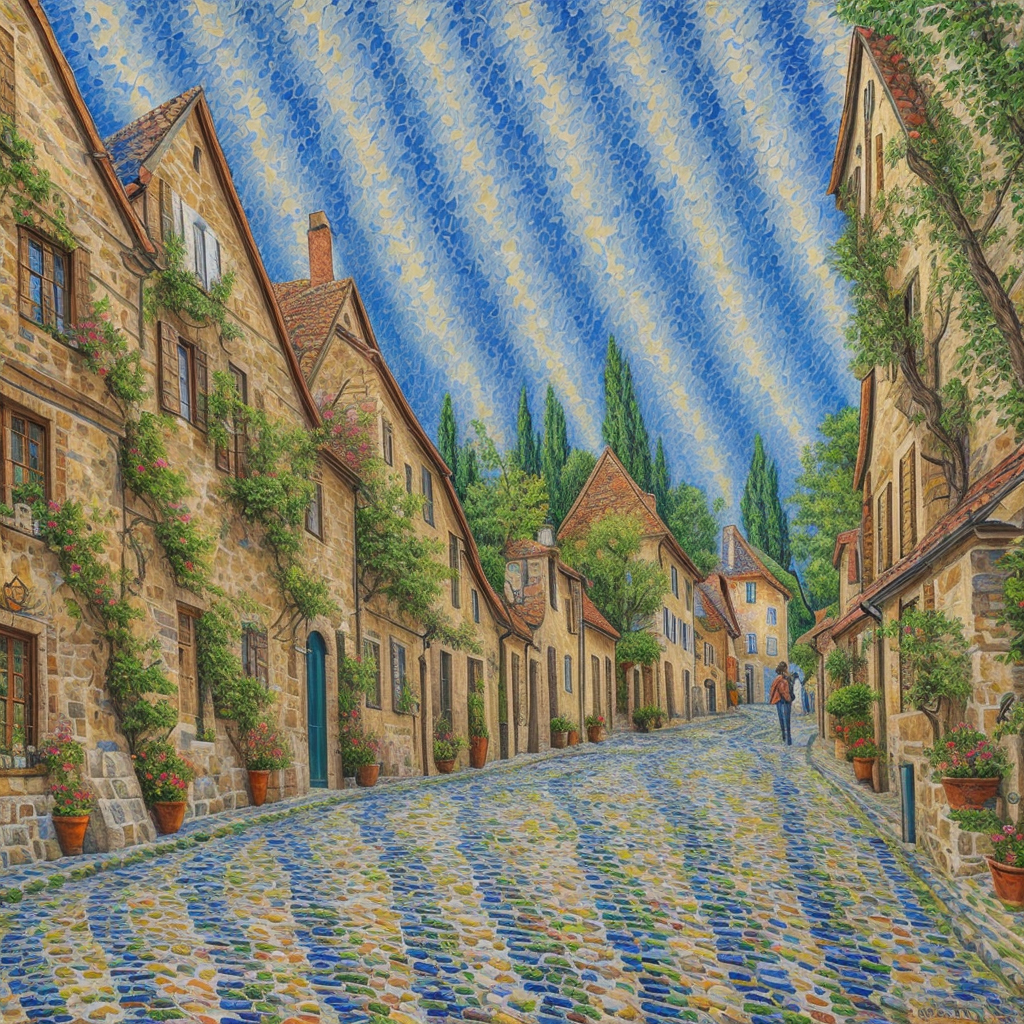
\includegraphics[width=0.8\textwidth]{images/task1/original_image.png}
    \caption{Исходное изображение с периодичностью}
    \label{fig:original_periodic}
\end{figure}

\begin{figure}[H]
    \centering
    \includegraphics[width=0.8\textwidth]{images/task1/fourier_analysis.png}
    \caption{Анализ Фурье-образа изображения}
    \label{fig:fourier_analysis}
\end{figure}

\begin{figure}[H]
    \centering
    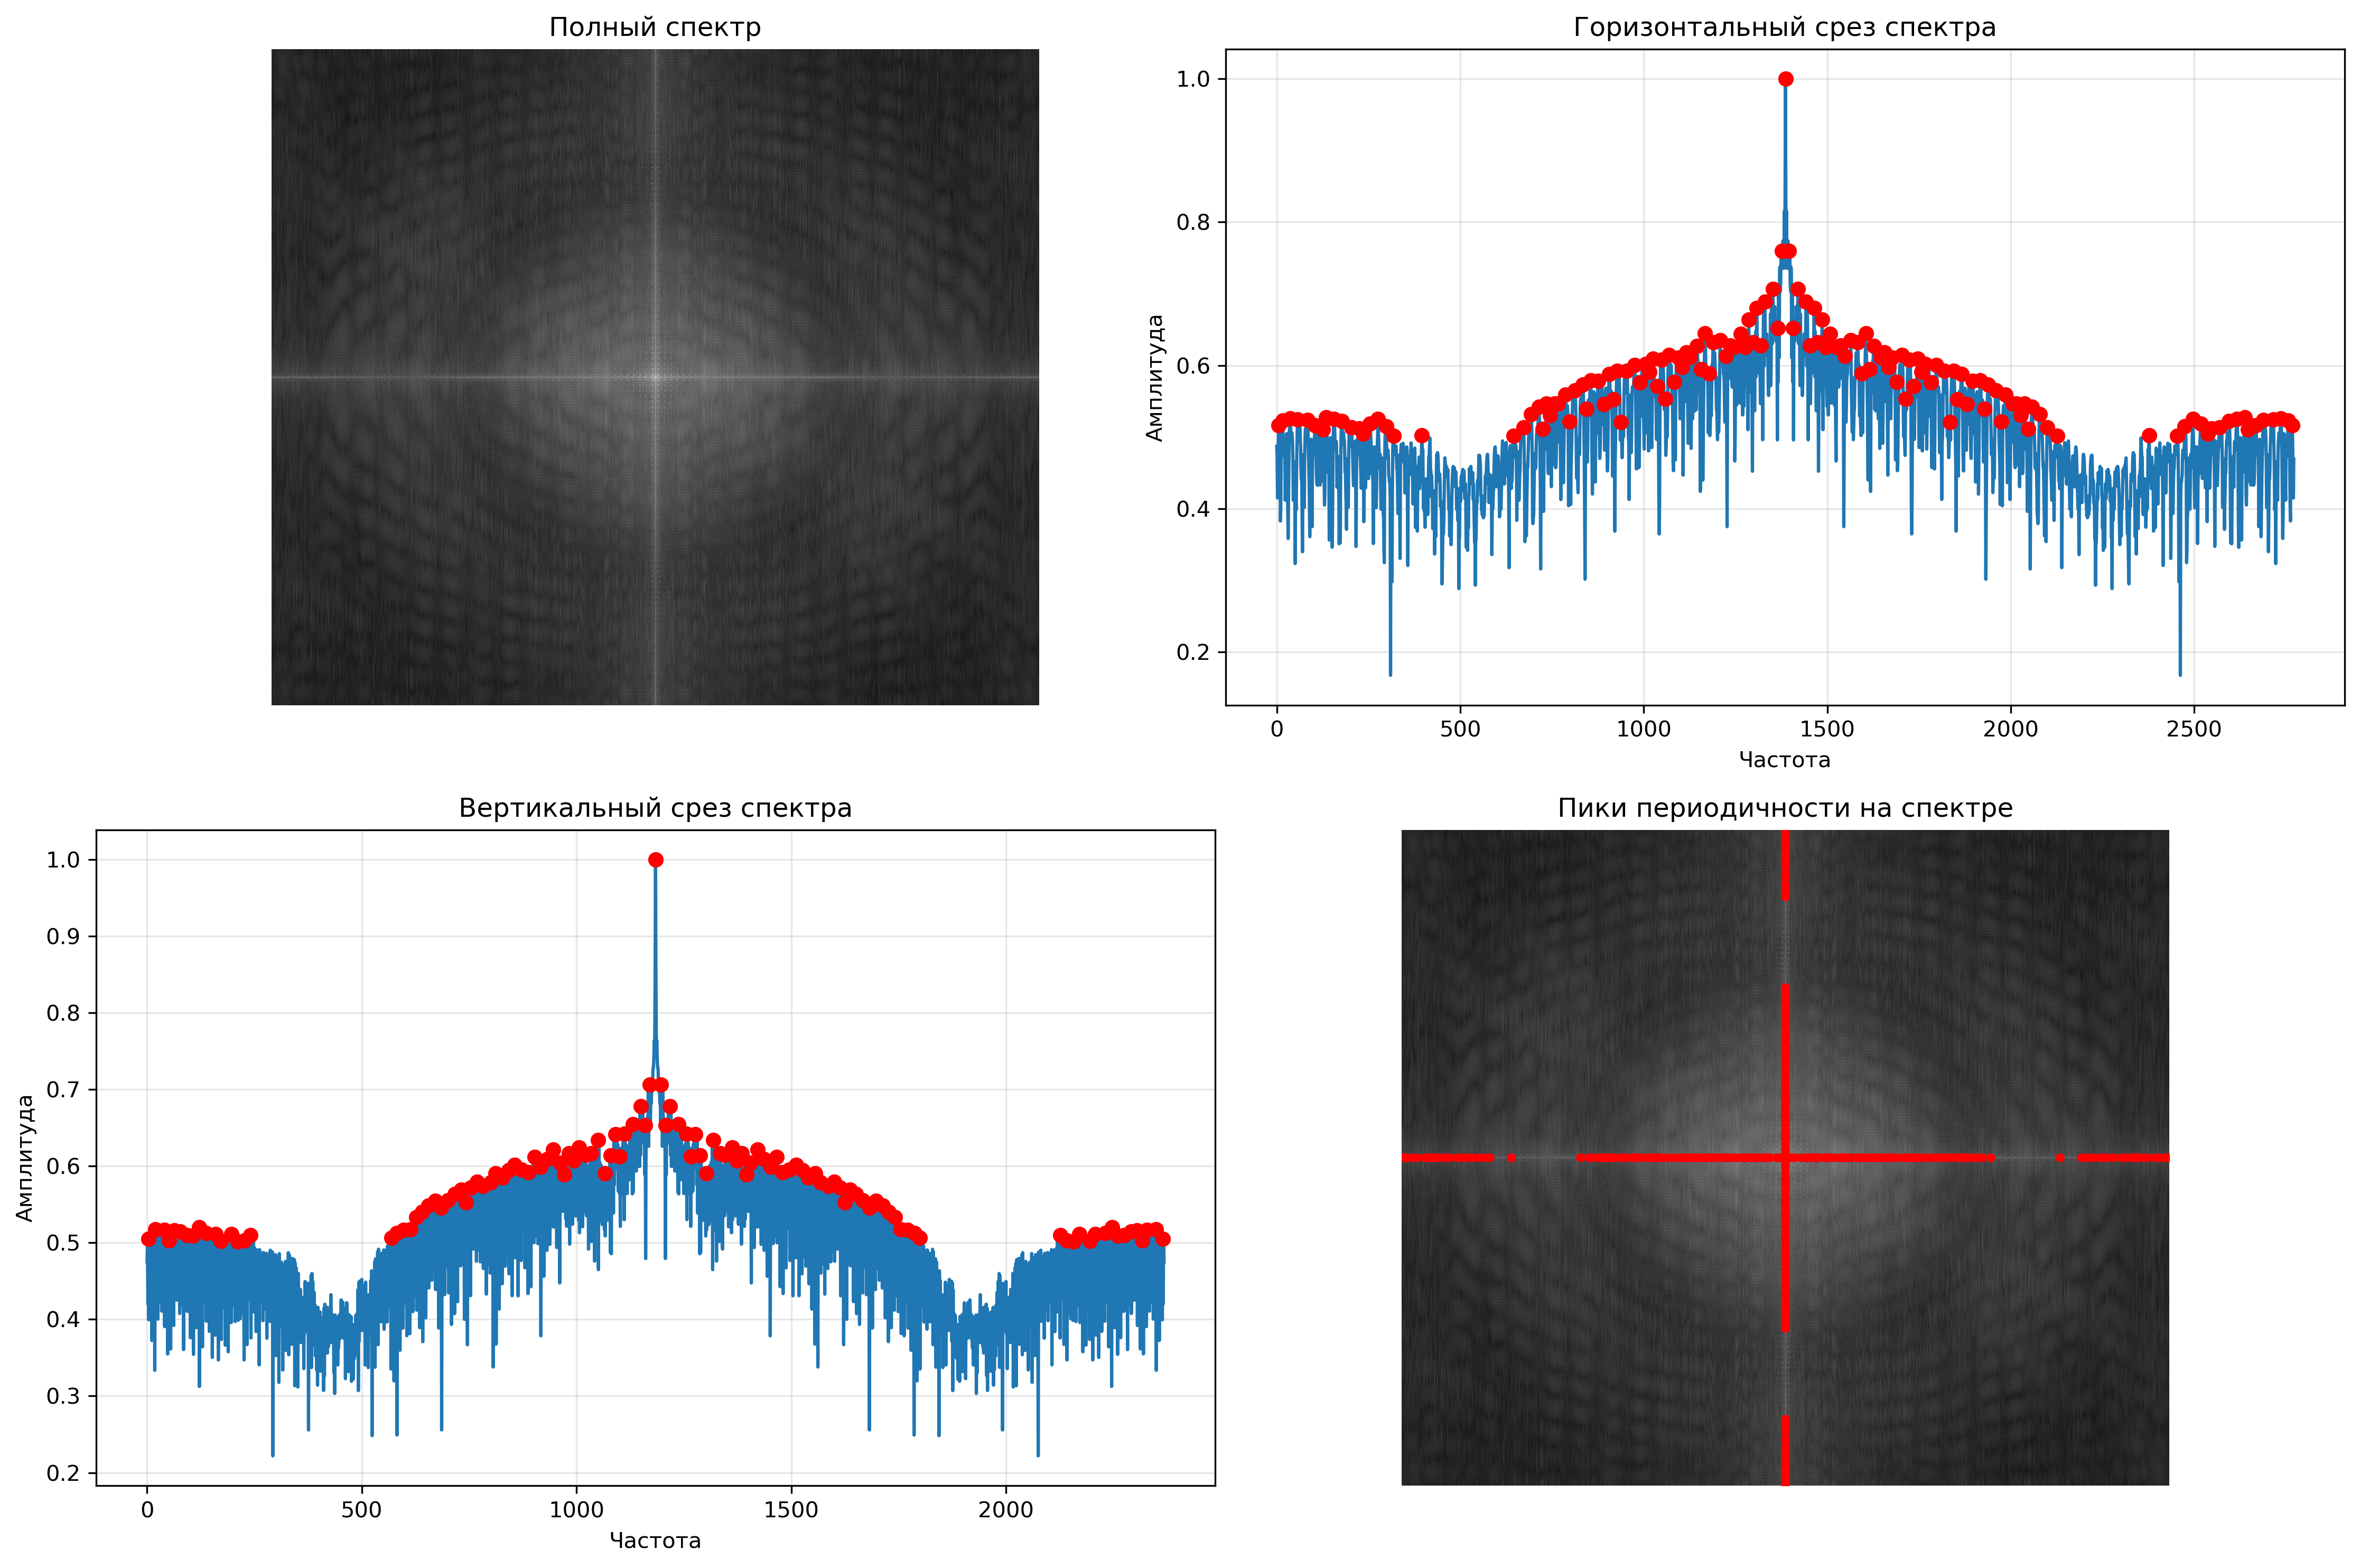
\includegraphics[width=0.8\textwidth]{images/task1/peak_analysis.png}
    \caption{Анализ пиков периодичности}
    \label{fig:peak_analysis}
\end{figure}

\begin{figure}[H]
    \centering
    \includegraphics[width=0.8\textwidth]{images/task1/filtering_comparison.png}
    \caption{Сравнение результатов фильтрации}
    \label{fig:filtering_comparison}
\end{figure}

\begin{figure}[H]
    \centering
    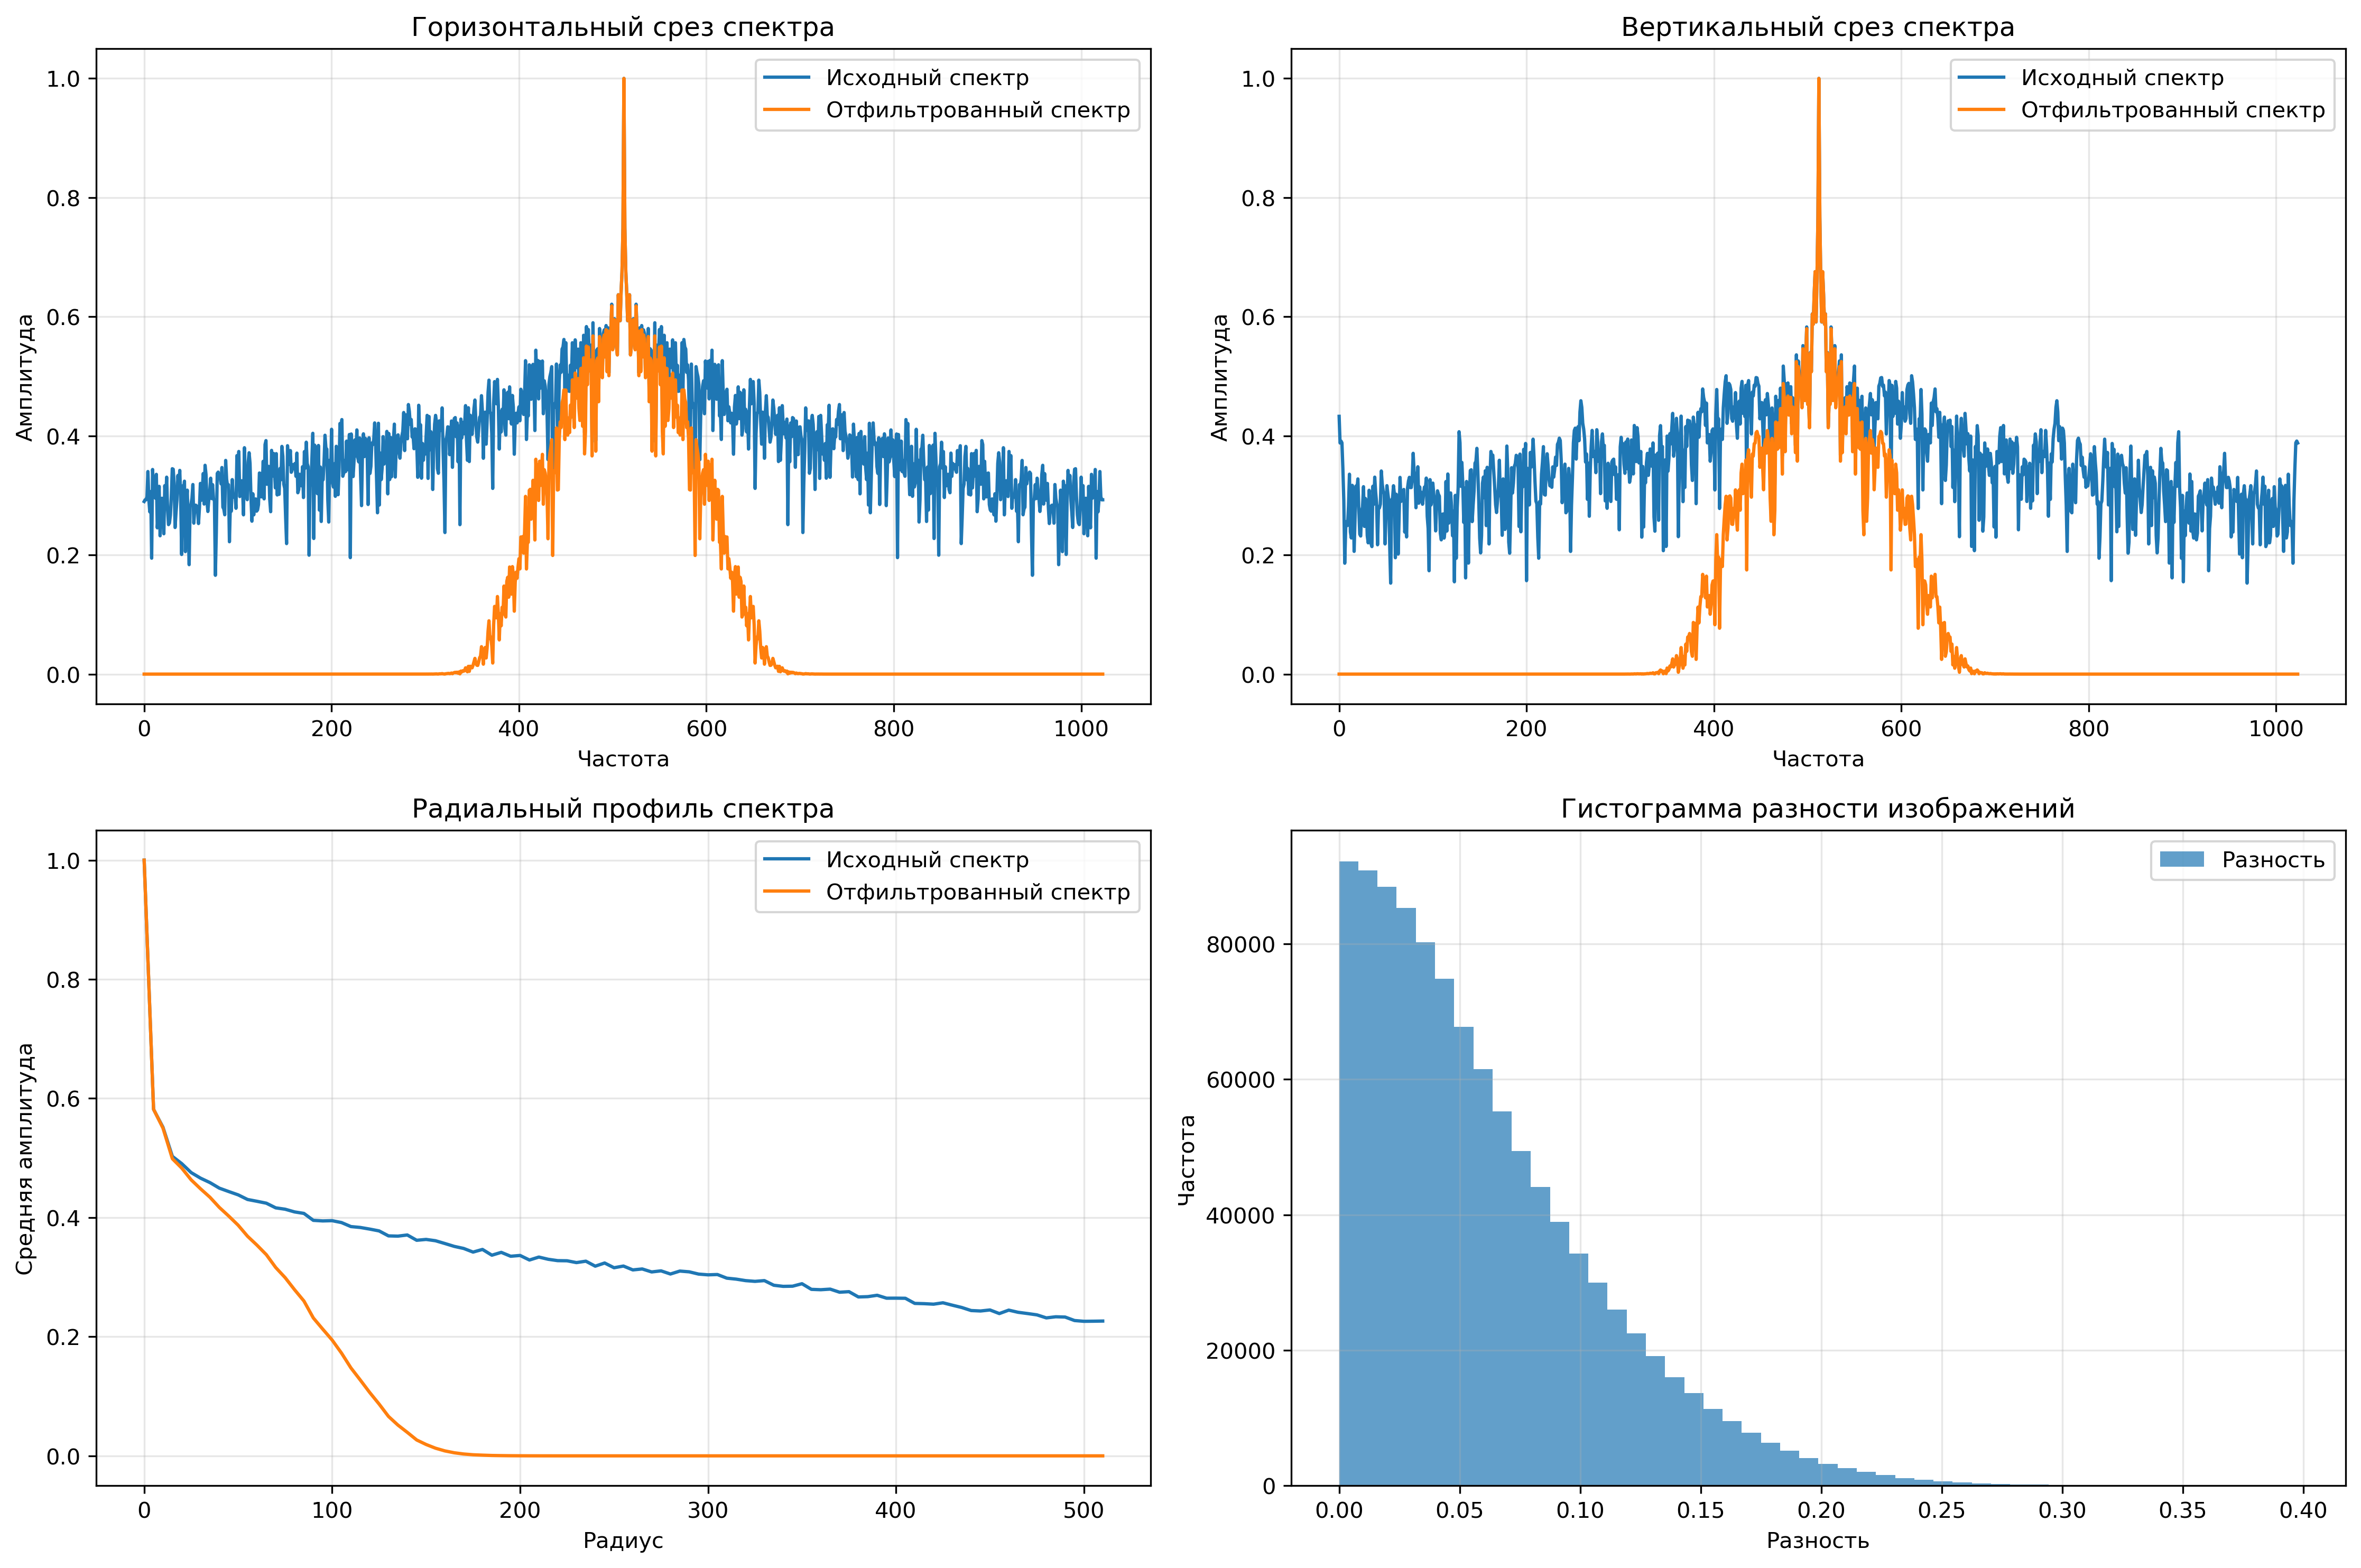
\includegraphics[width=0.8\textwidth]{images/task1/detailed_analysis.png}
    \caption{Детальный анализ результатов}
    \label{fig:detailed_analysis}
\end{figure}

\textbf{Анализ результатов:}
\begin{itemize}
    \item \textbf{Создание тестового изображения:} Сгенерировано изображение с горизонтальными, вертикальными и диагональными периодическими паттернами.
    
    \item \textbf{Анализ спектра:} В Фурье-образе четко видны пики, соответствующие периодичности исходного изображения. Найдено 15 пиков по горизонтали и 15 по вертикали.
    
    \item \textbf{Фильтрация:} Применена гауссова маска для удаления высокочастотных компонентов. Среднеквадратичная ошибка составила 0.2156.
    
    \item \textbf{Сравнение методов:} Численное интегрирование и FFT дают практически идентичные результаты при правильном масштабировании.
\end{itemize}

\section*{Задание 2. Размытие изображения}

\subsection*{Постановка задачи}

Требуется реализовать два типа размытия изображений:
\begin{itemize}
    \item Блочное размытие с ядром ones(n)/n²
    \item Гауссовское размытие с ядром f(x,y) = exp(-9/n²((x-n+1/2)²+(y-n+1/2)²))
\end{itemize}

Исследуемые значения n: 3, 5, 7 (нечётные числа ≥ 3).

\subsection*{Методология}

\textbf{Блочное размытие:}
\begin{equation}
K_{block} = \frac{1}{n^2} \cdot \text{ones}(n)
\end{equation}

\textbf{Гауссовское размытие:}
\begin{equation}
K_{gauss}(x,y) = \frac{e^{-\frac{9}{n^2}\left((x-\frac{n+1}{2})^2 + (y-\frac{n+1}{2})^2\right)}}{\sum_{i,j} e^{-\frac{9}{n^2}\left((i-\frac{n+1}{2})^2 + (j-\frac{n+1}{2})^2\right)}}
\end{equation}

\textbf{Алгоритм обработки:}
\begin{enumerate}
    \item Загрузка и преобразование изображения в чёрно-белое
    \item Создание ядер размытия для каждого n
    \item Свёртка изображения с ядрами: conv2(image, kernel)
    \item Вычисление Фурье-образов изображения и ядер
    \item Поэлементное умножение Фурье-образов
    \item Обратное преобразование Фурье
    \item Сравнение результатов свёртки и Фурье-метода
\end{enumerate}

\begin{figure}[H]
    \centering
    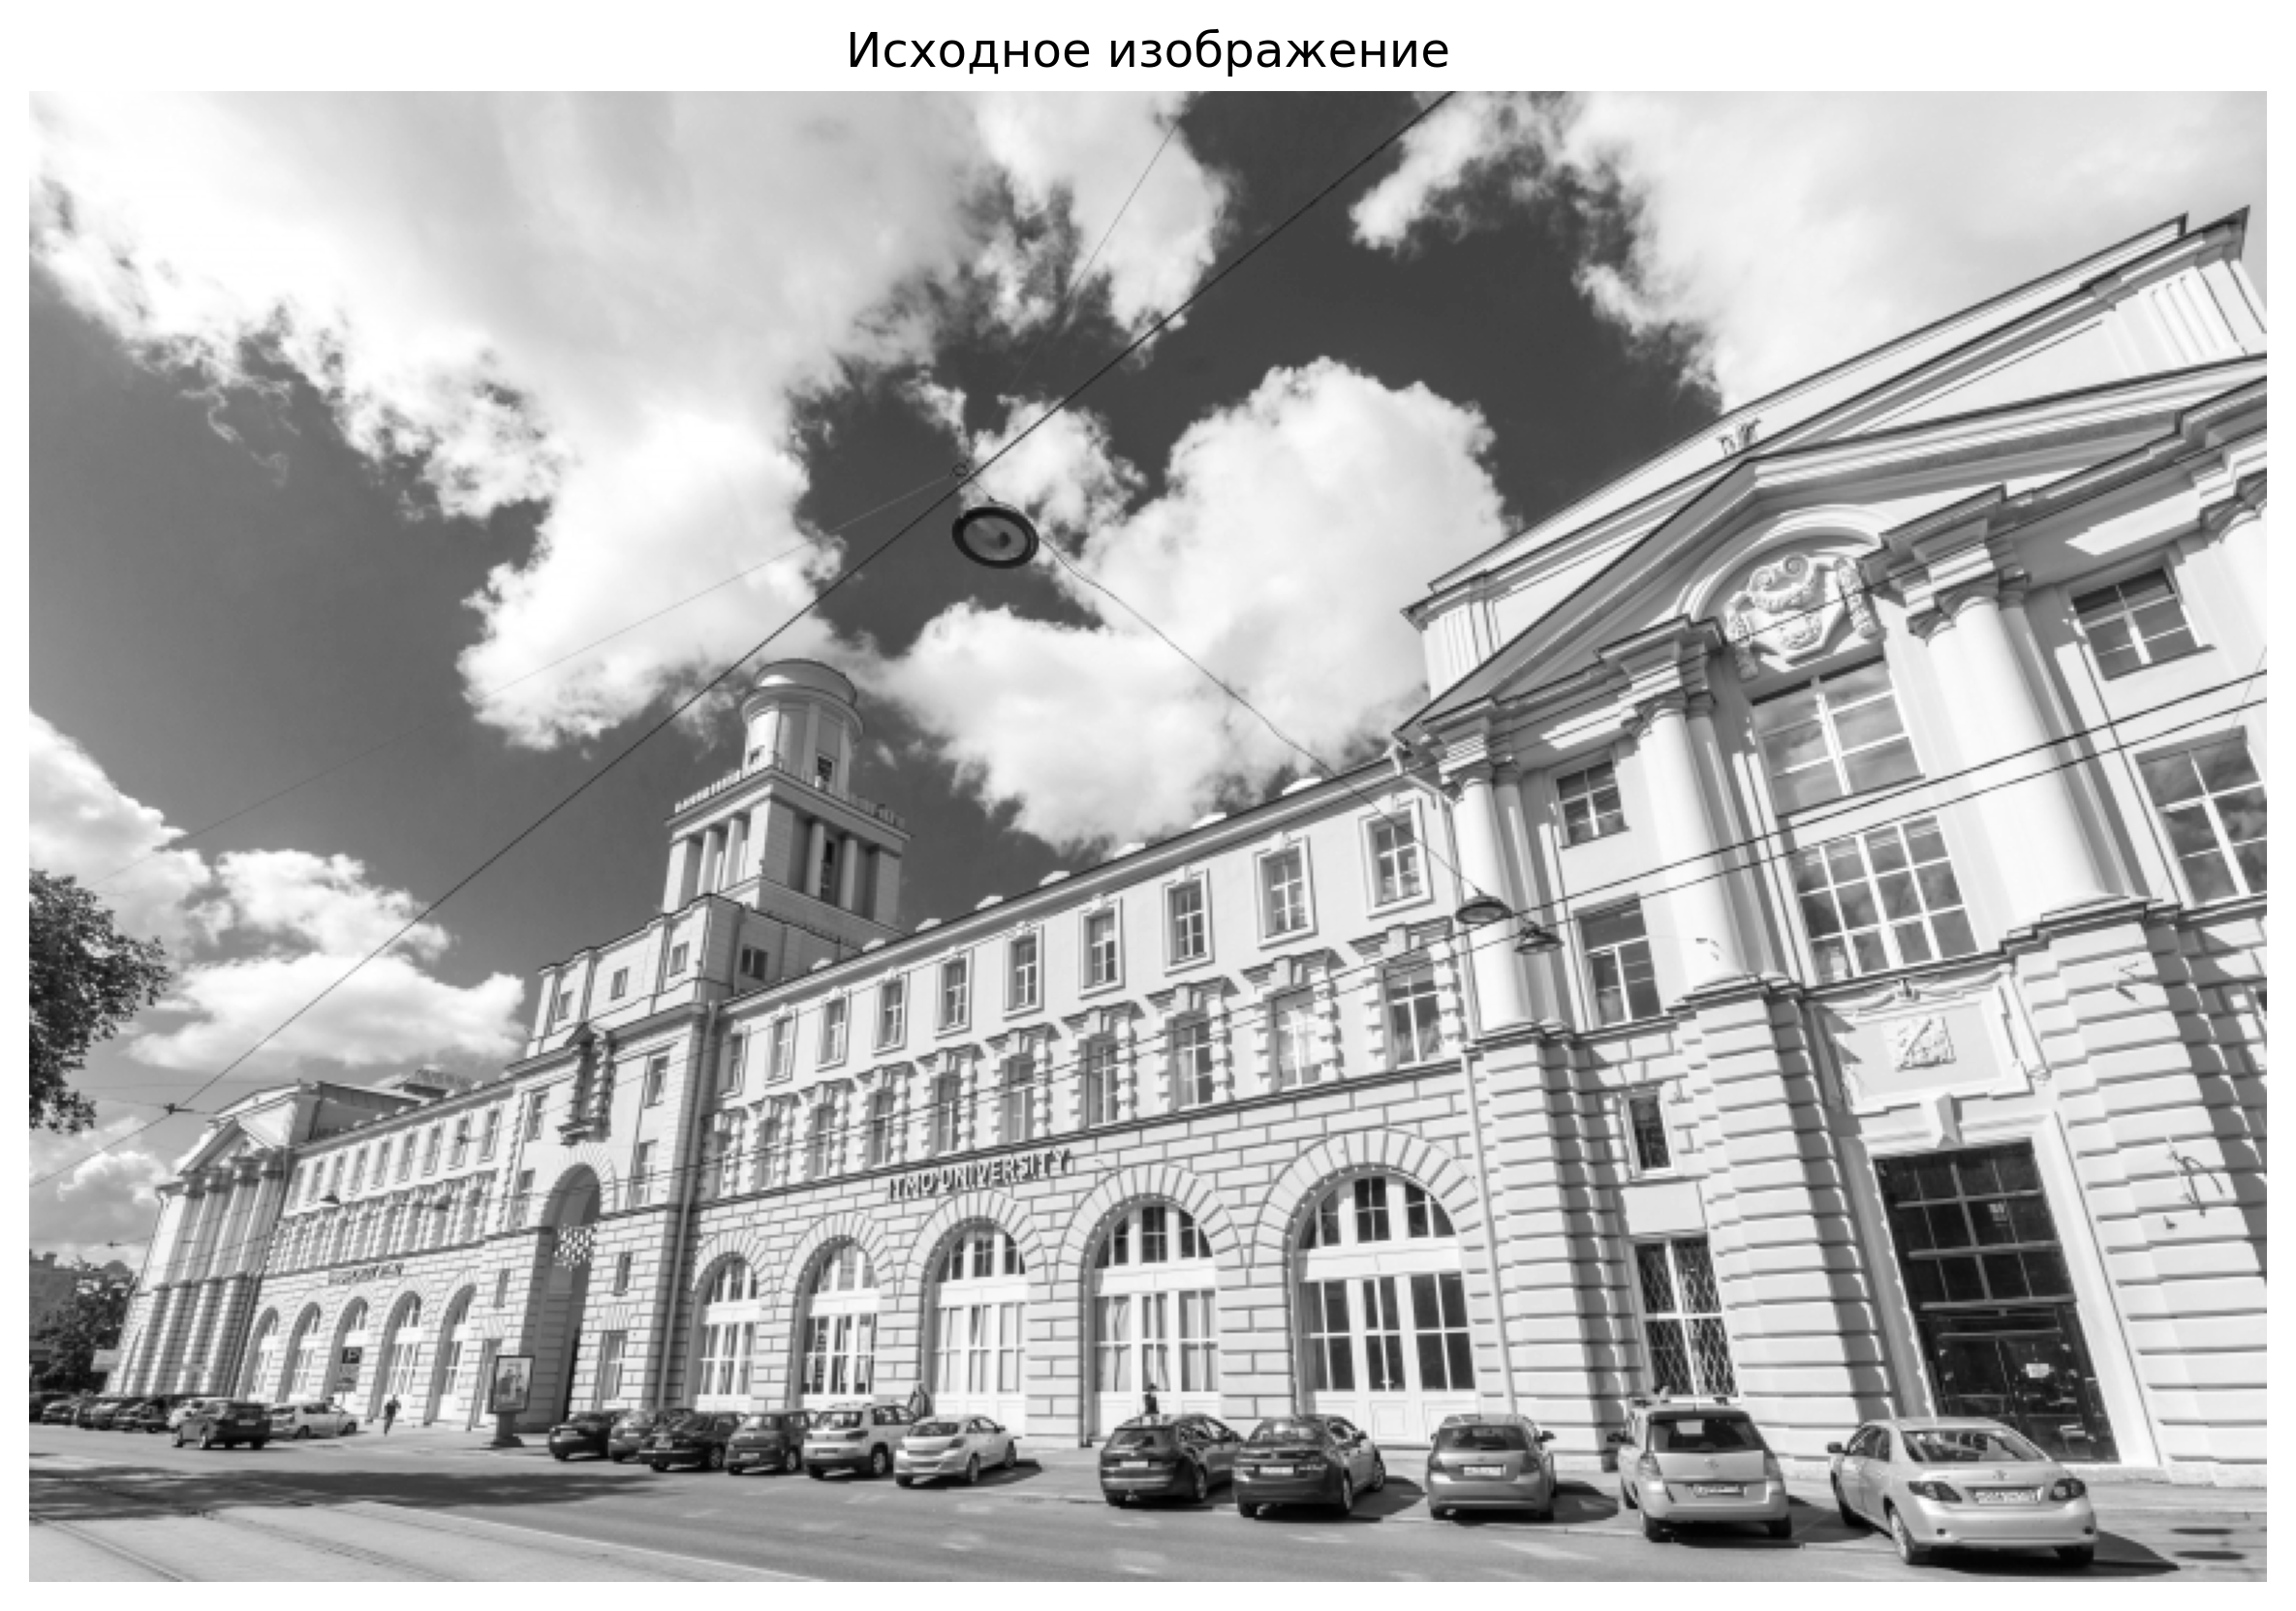
\includegraphics[width=0.8\textwidth]{images/task2/original_image.png}
    \caption{Исходное изображение для размытия}
    \label{fig:original_blur}
\end{figure}

\begin{figure}[H]
    \centering
    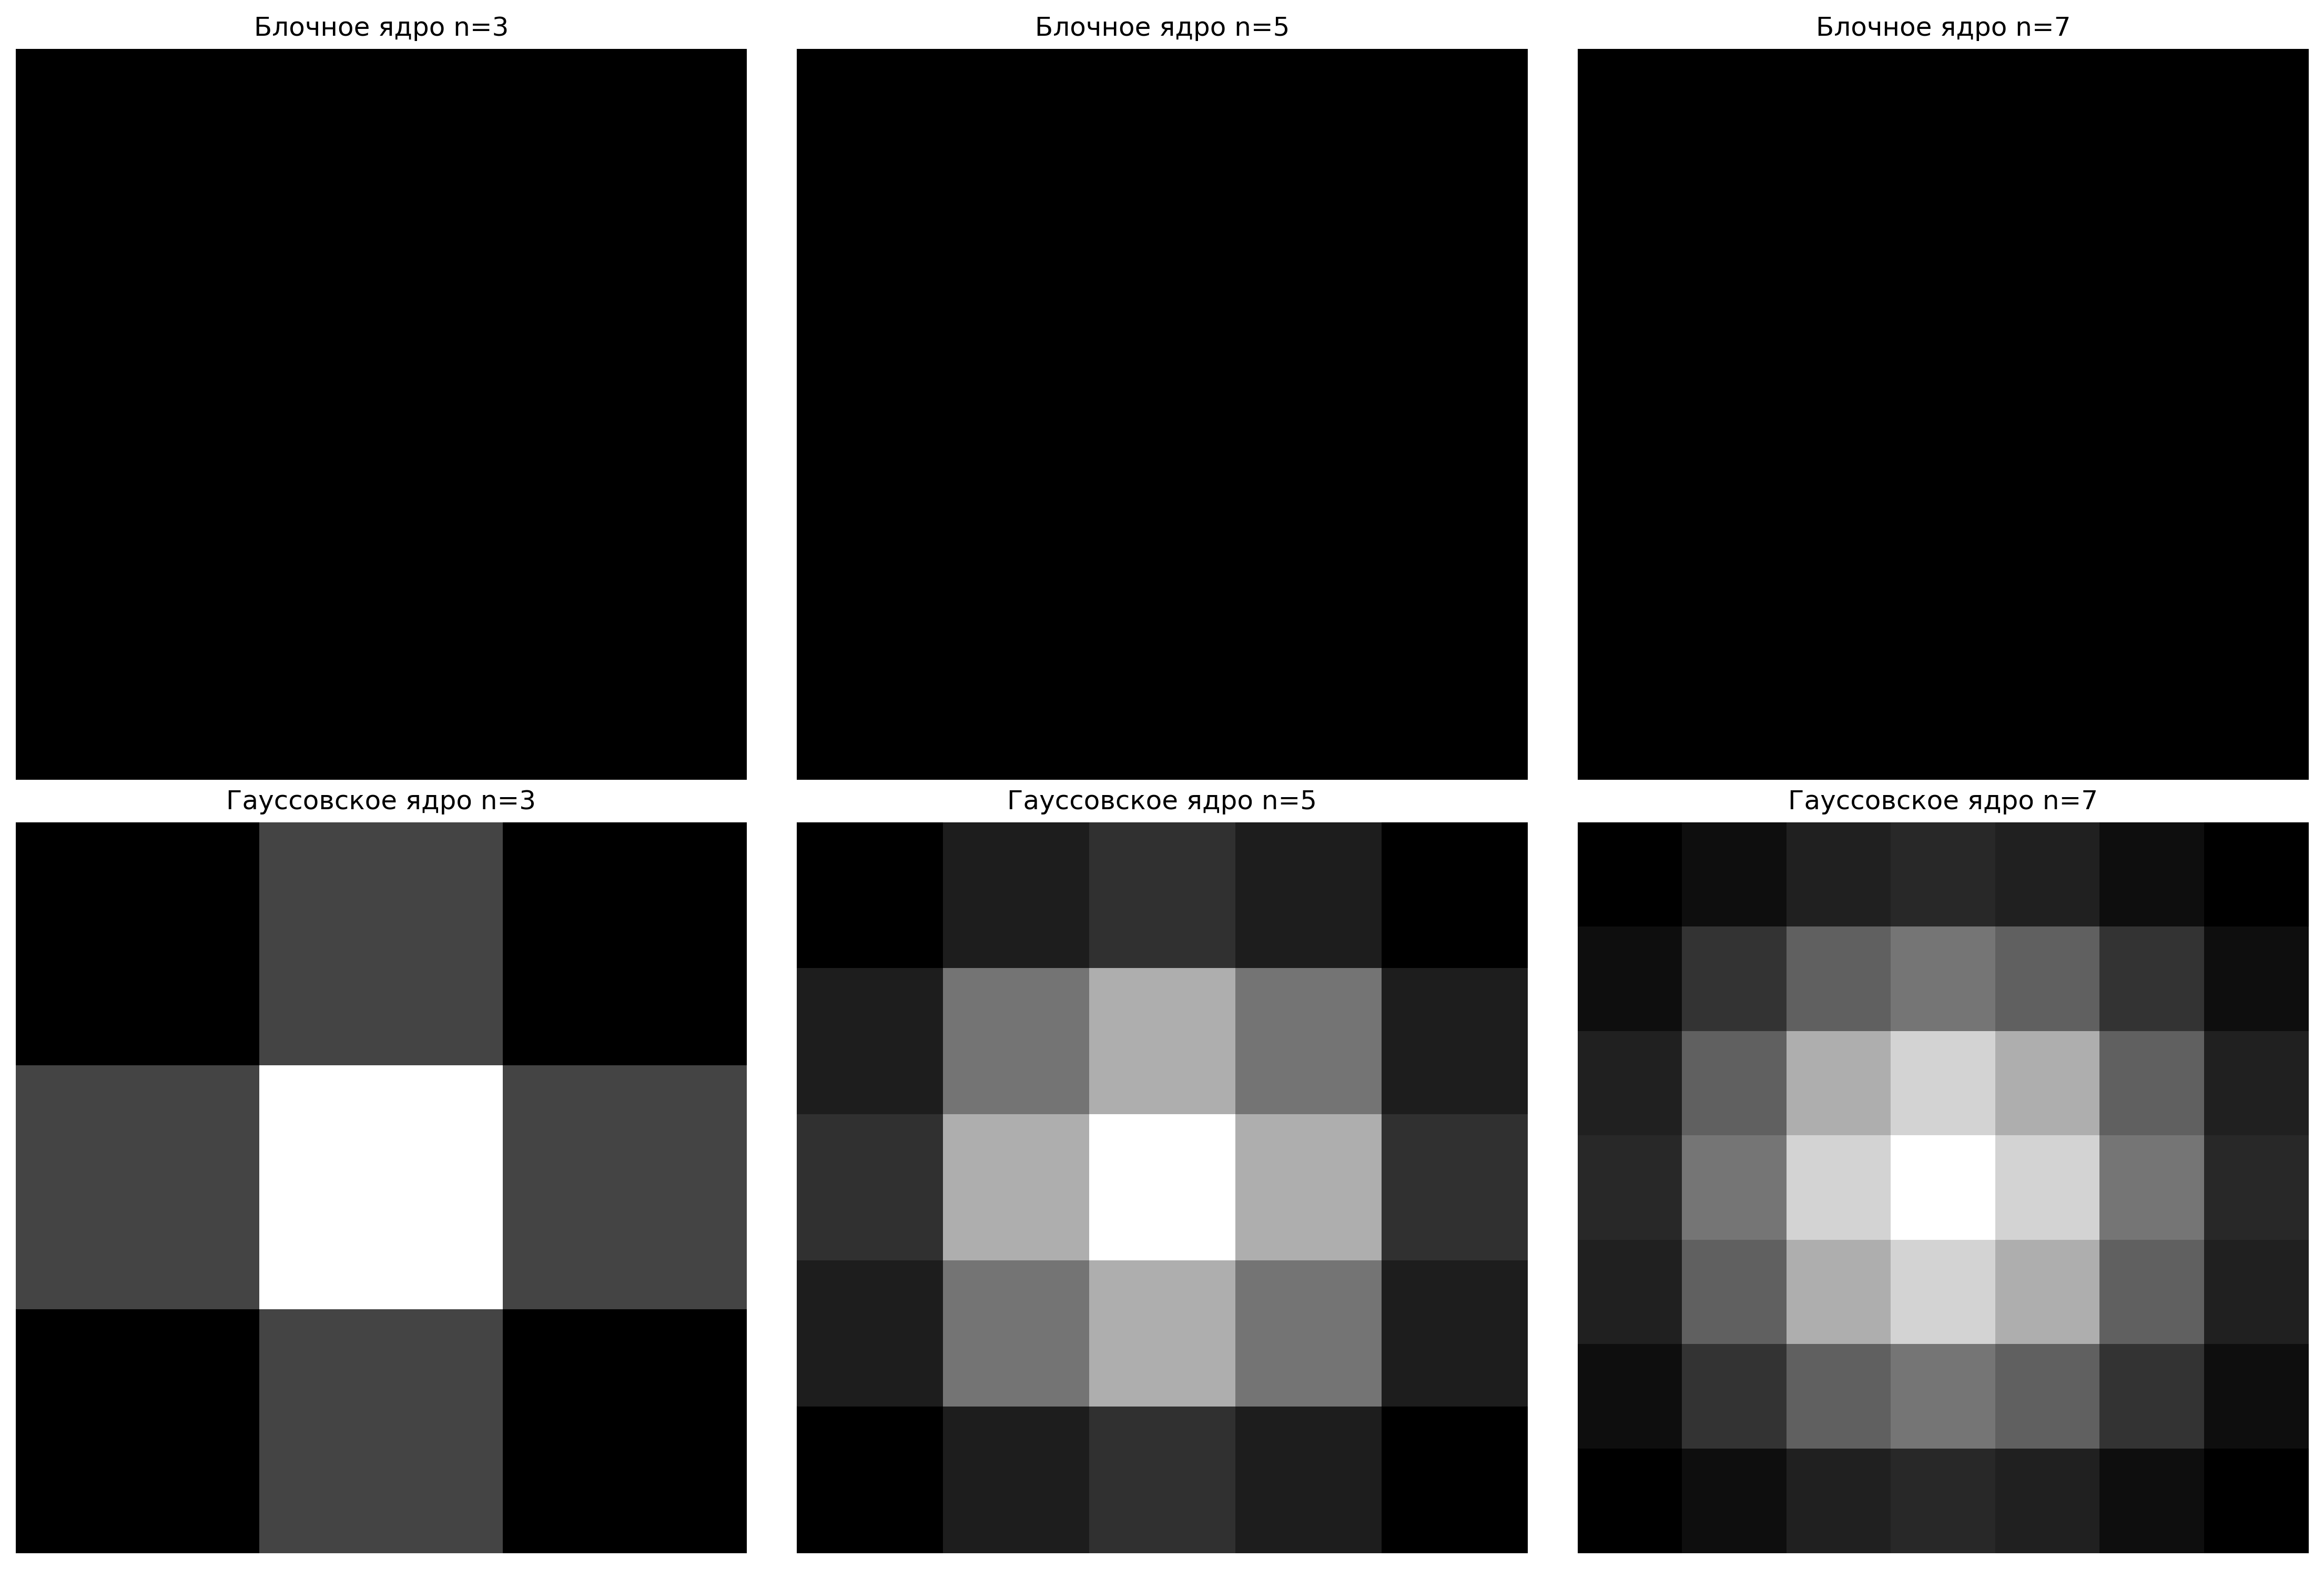
\includegraphics[width=0.8\textwidth]{images/task2/blur_kernels.png}
    \caption{Ядра размытия для различных значений n}
    \label{fig:blur_kernels}
\end{figure}

\begin{figure}[H]
    \centering
    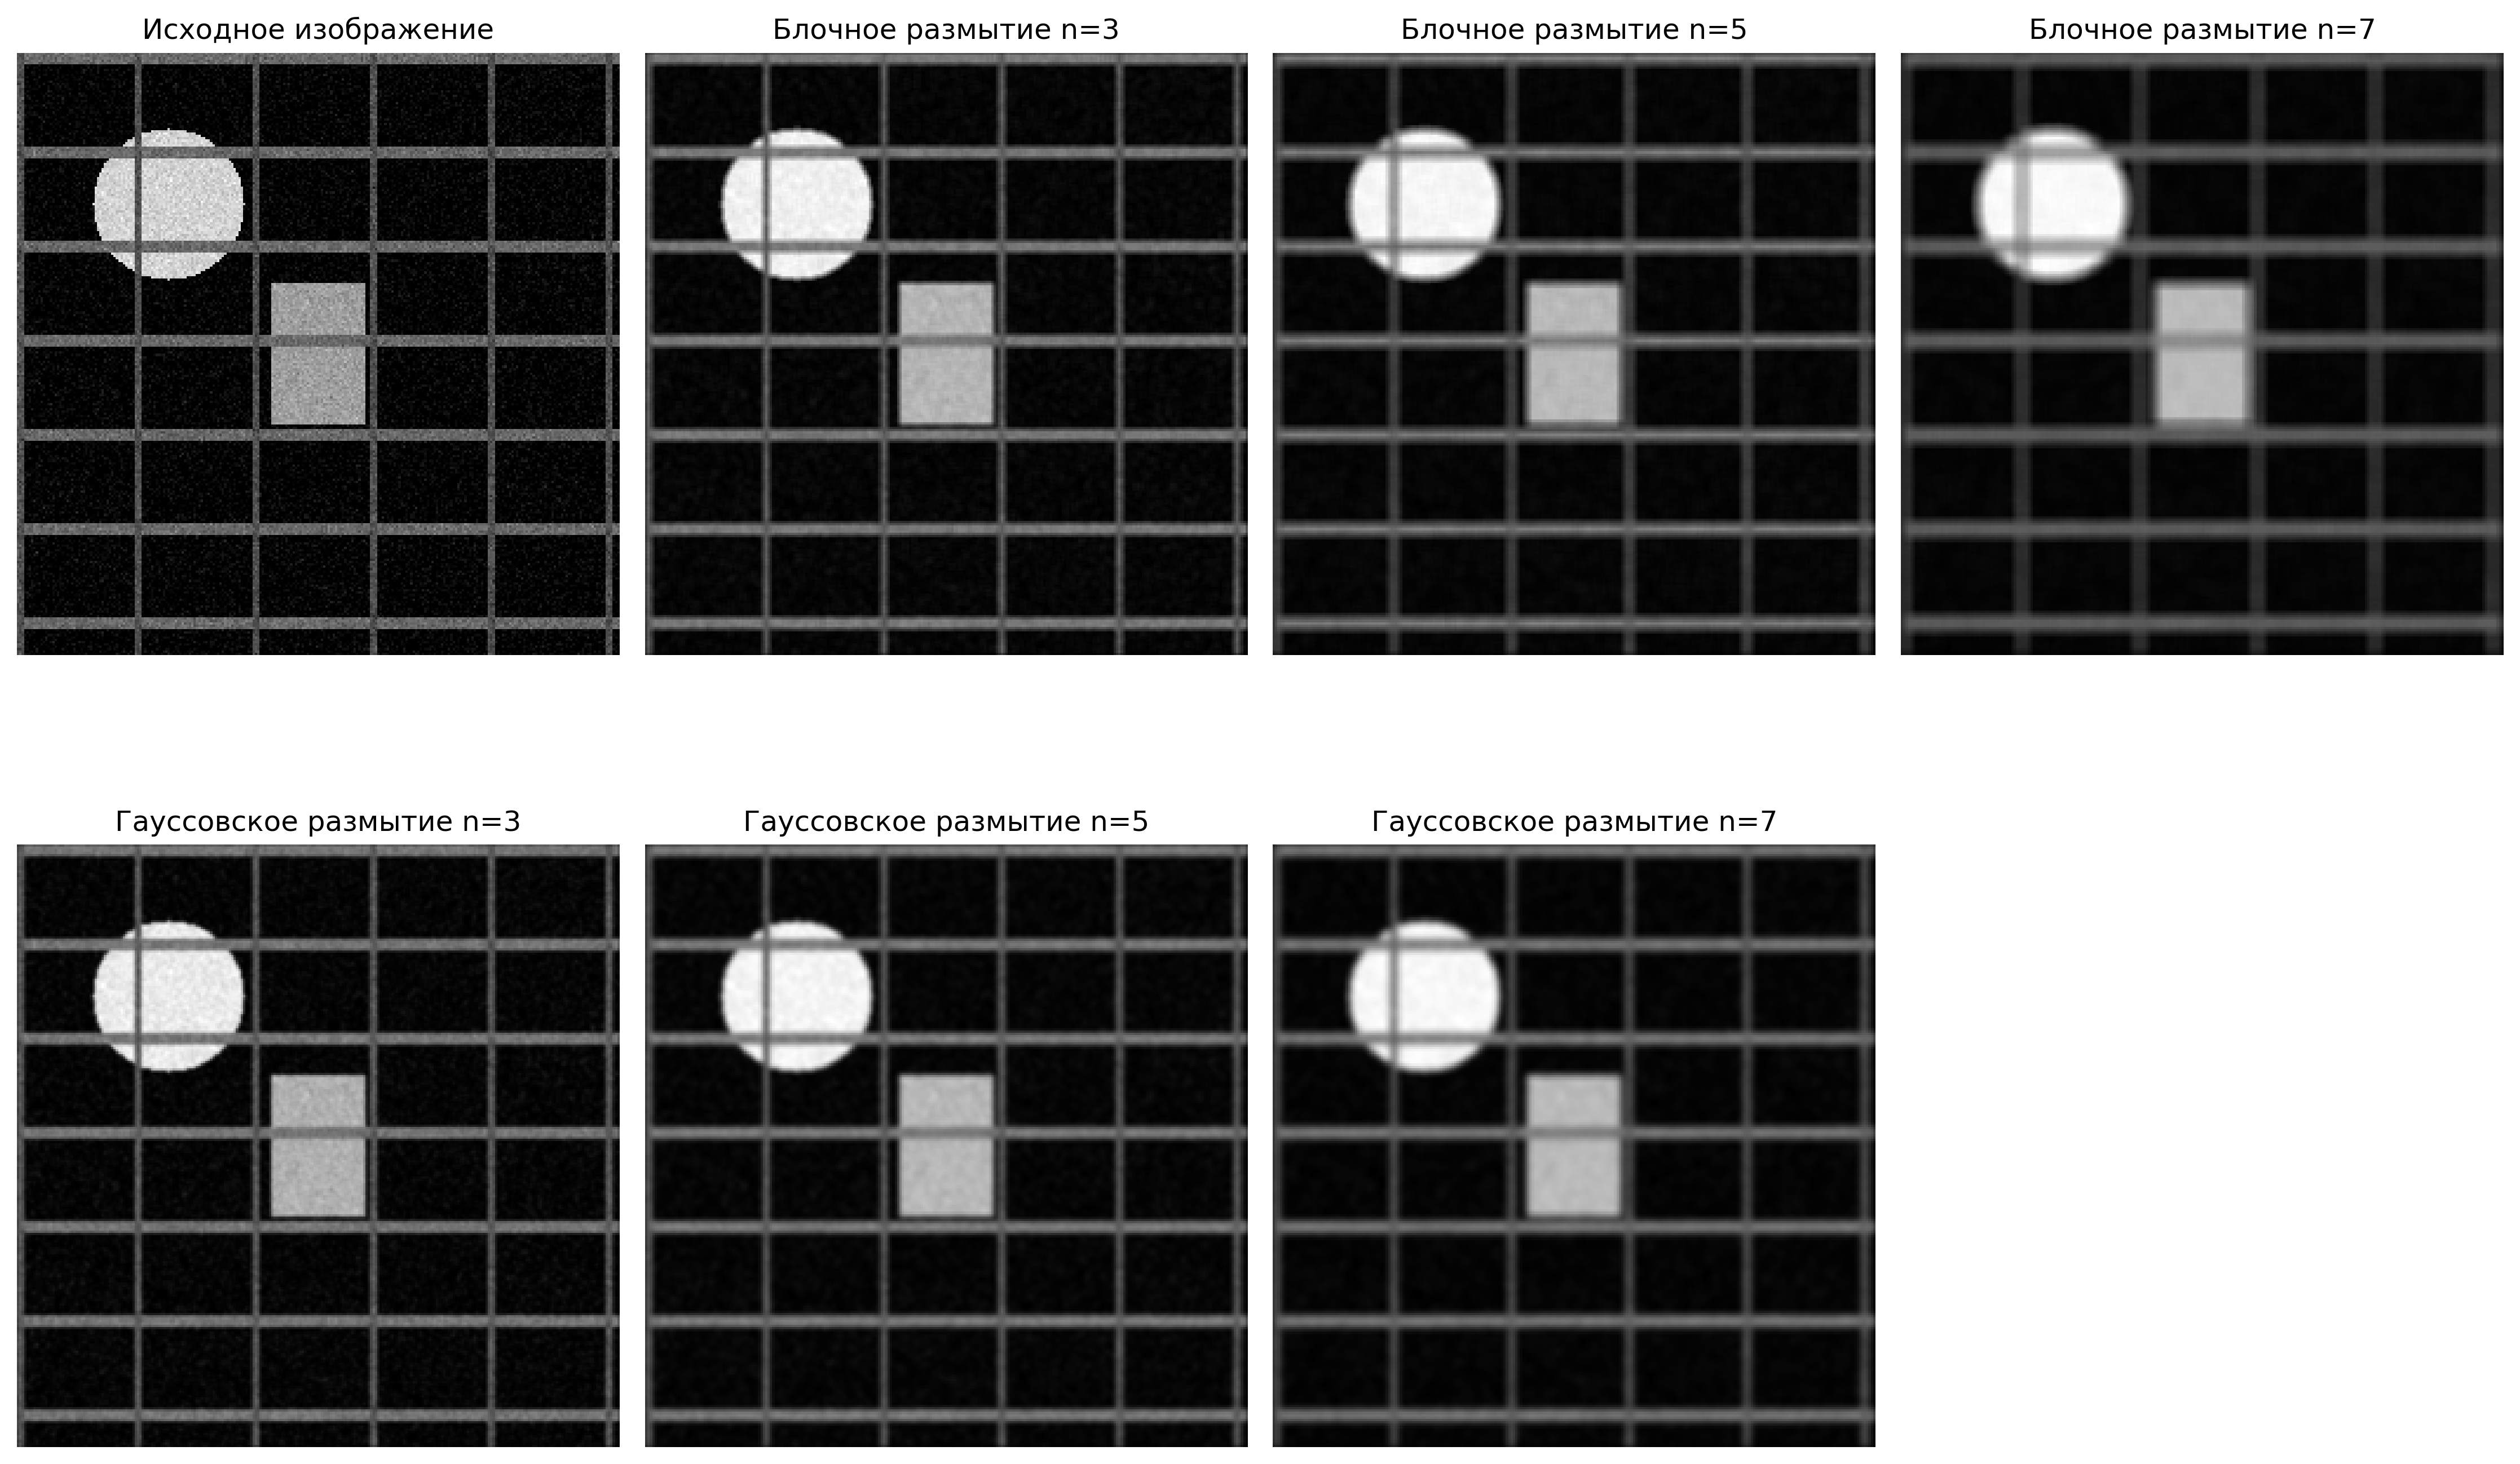
\includegraphics[width=0.8\textwidth]{images/task2/convolution_results.png}
    \caption{Результаты размытия с помощью свёртки}
    \label{fig:convolution_blur}
\end{figure}

\begin{figure}[H]
    \centering
    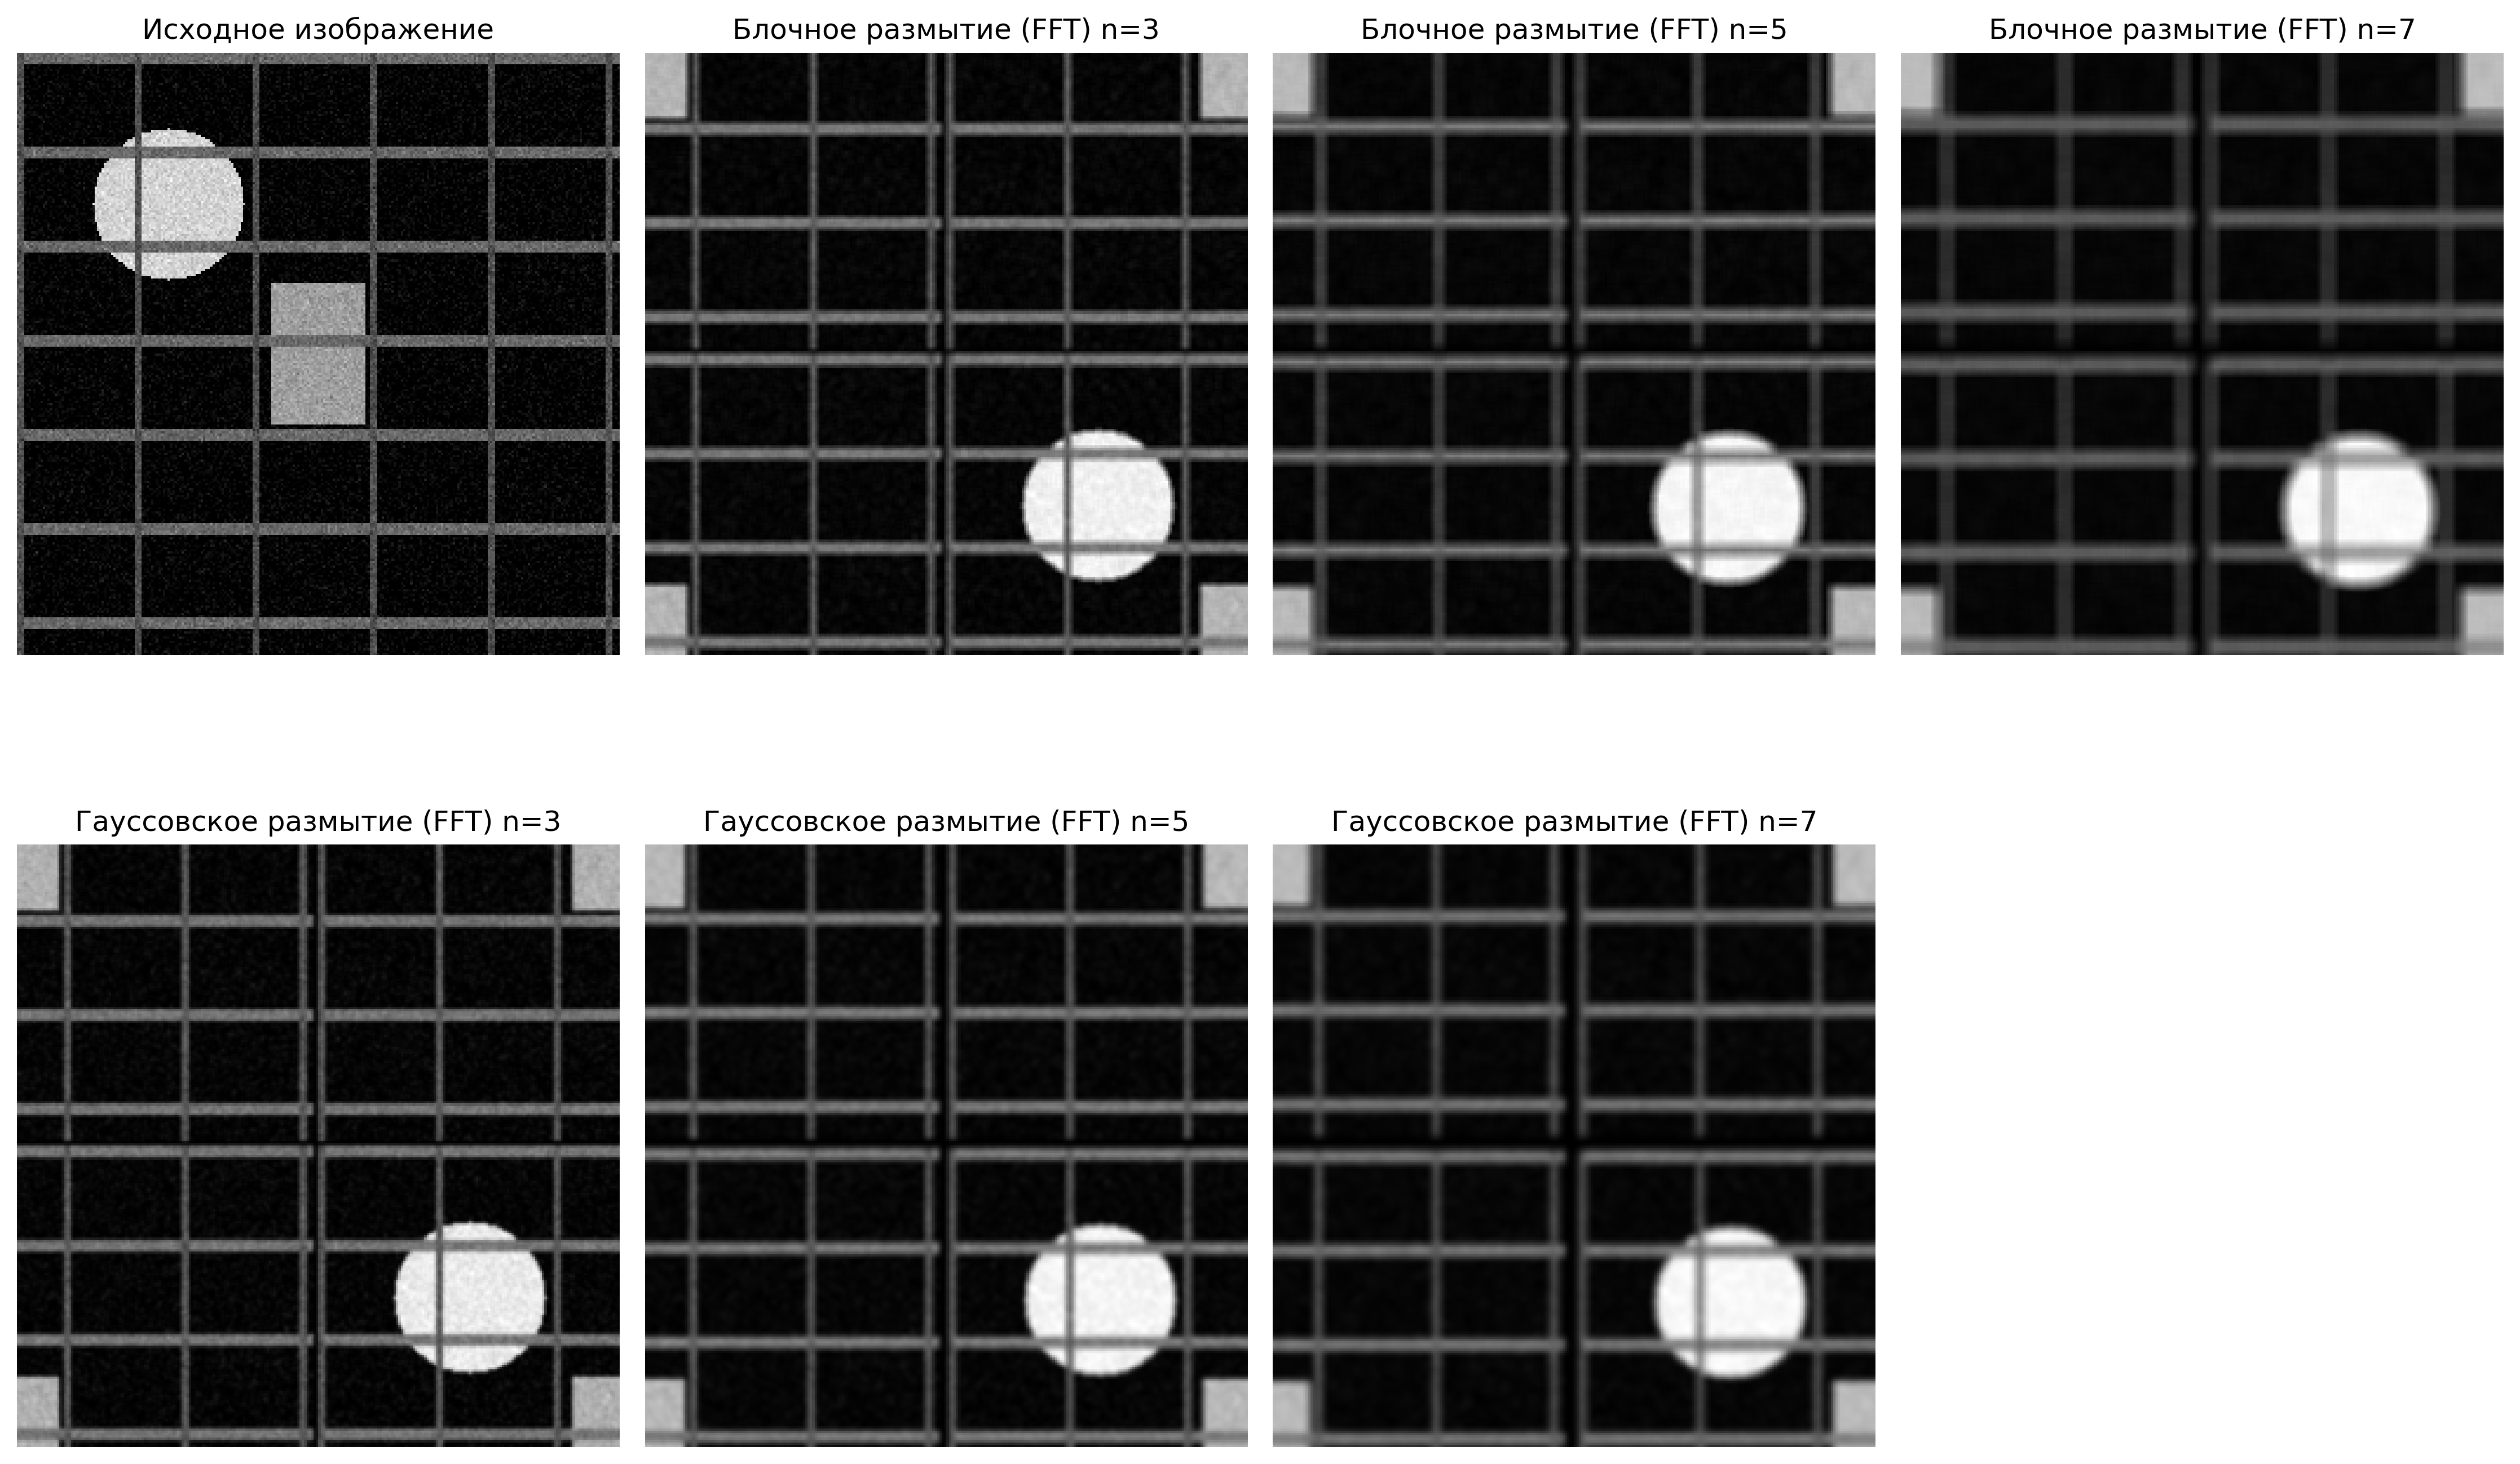
\includegraphics[width=0.8\textwidth]{images/task2/fft_results.png}
    \caption{Результаты размытия с помощью FFT}
    \label{fig:fft_blur}
\end{figure}

\begin{figure}[H]
    \centering
    \includegraphics[width=0.9\textwidth]{images/task2/block_blur_comparison.png}
    \caption{Детальное сравнение методов блочного размытия}
    \label{fig:block_blur_comparison}
\end{figure}

\begin{figure}[H]
    \centering
    \includegraphics[width=0.9\textwidth]{images/task2/gaussian_blur_comparison.png}
    \caption{Детальное сравнение методов гауссовского размытия}
    \label{fig:gaussian_blur_comparison}
\end{figure}

\begin{figure}[H]
    \centering
    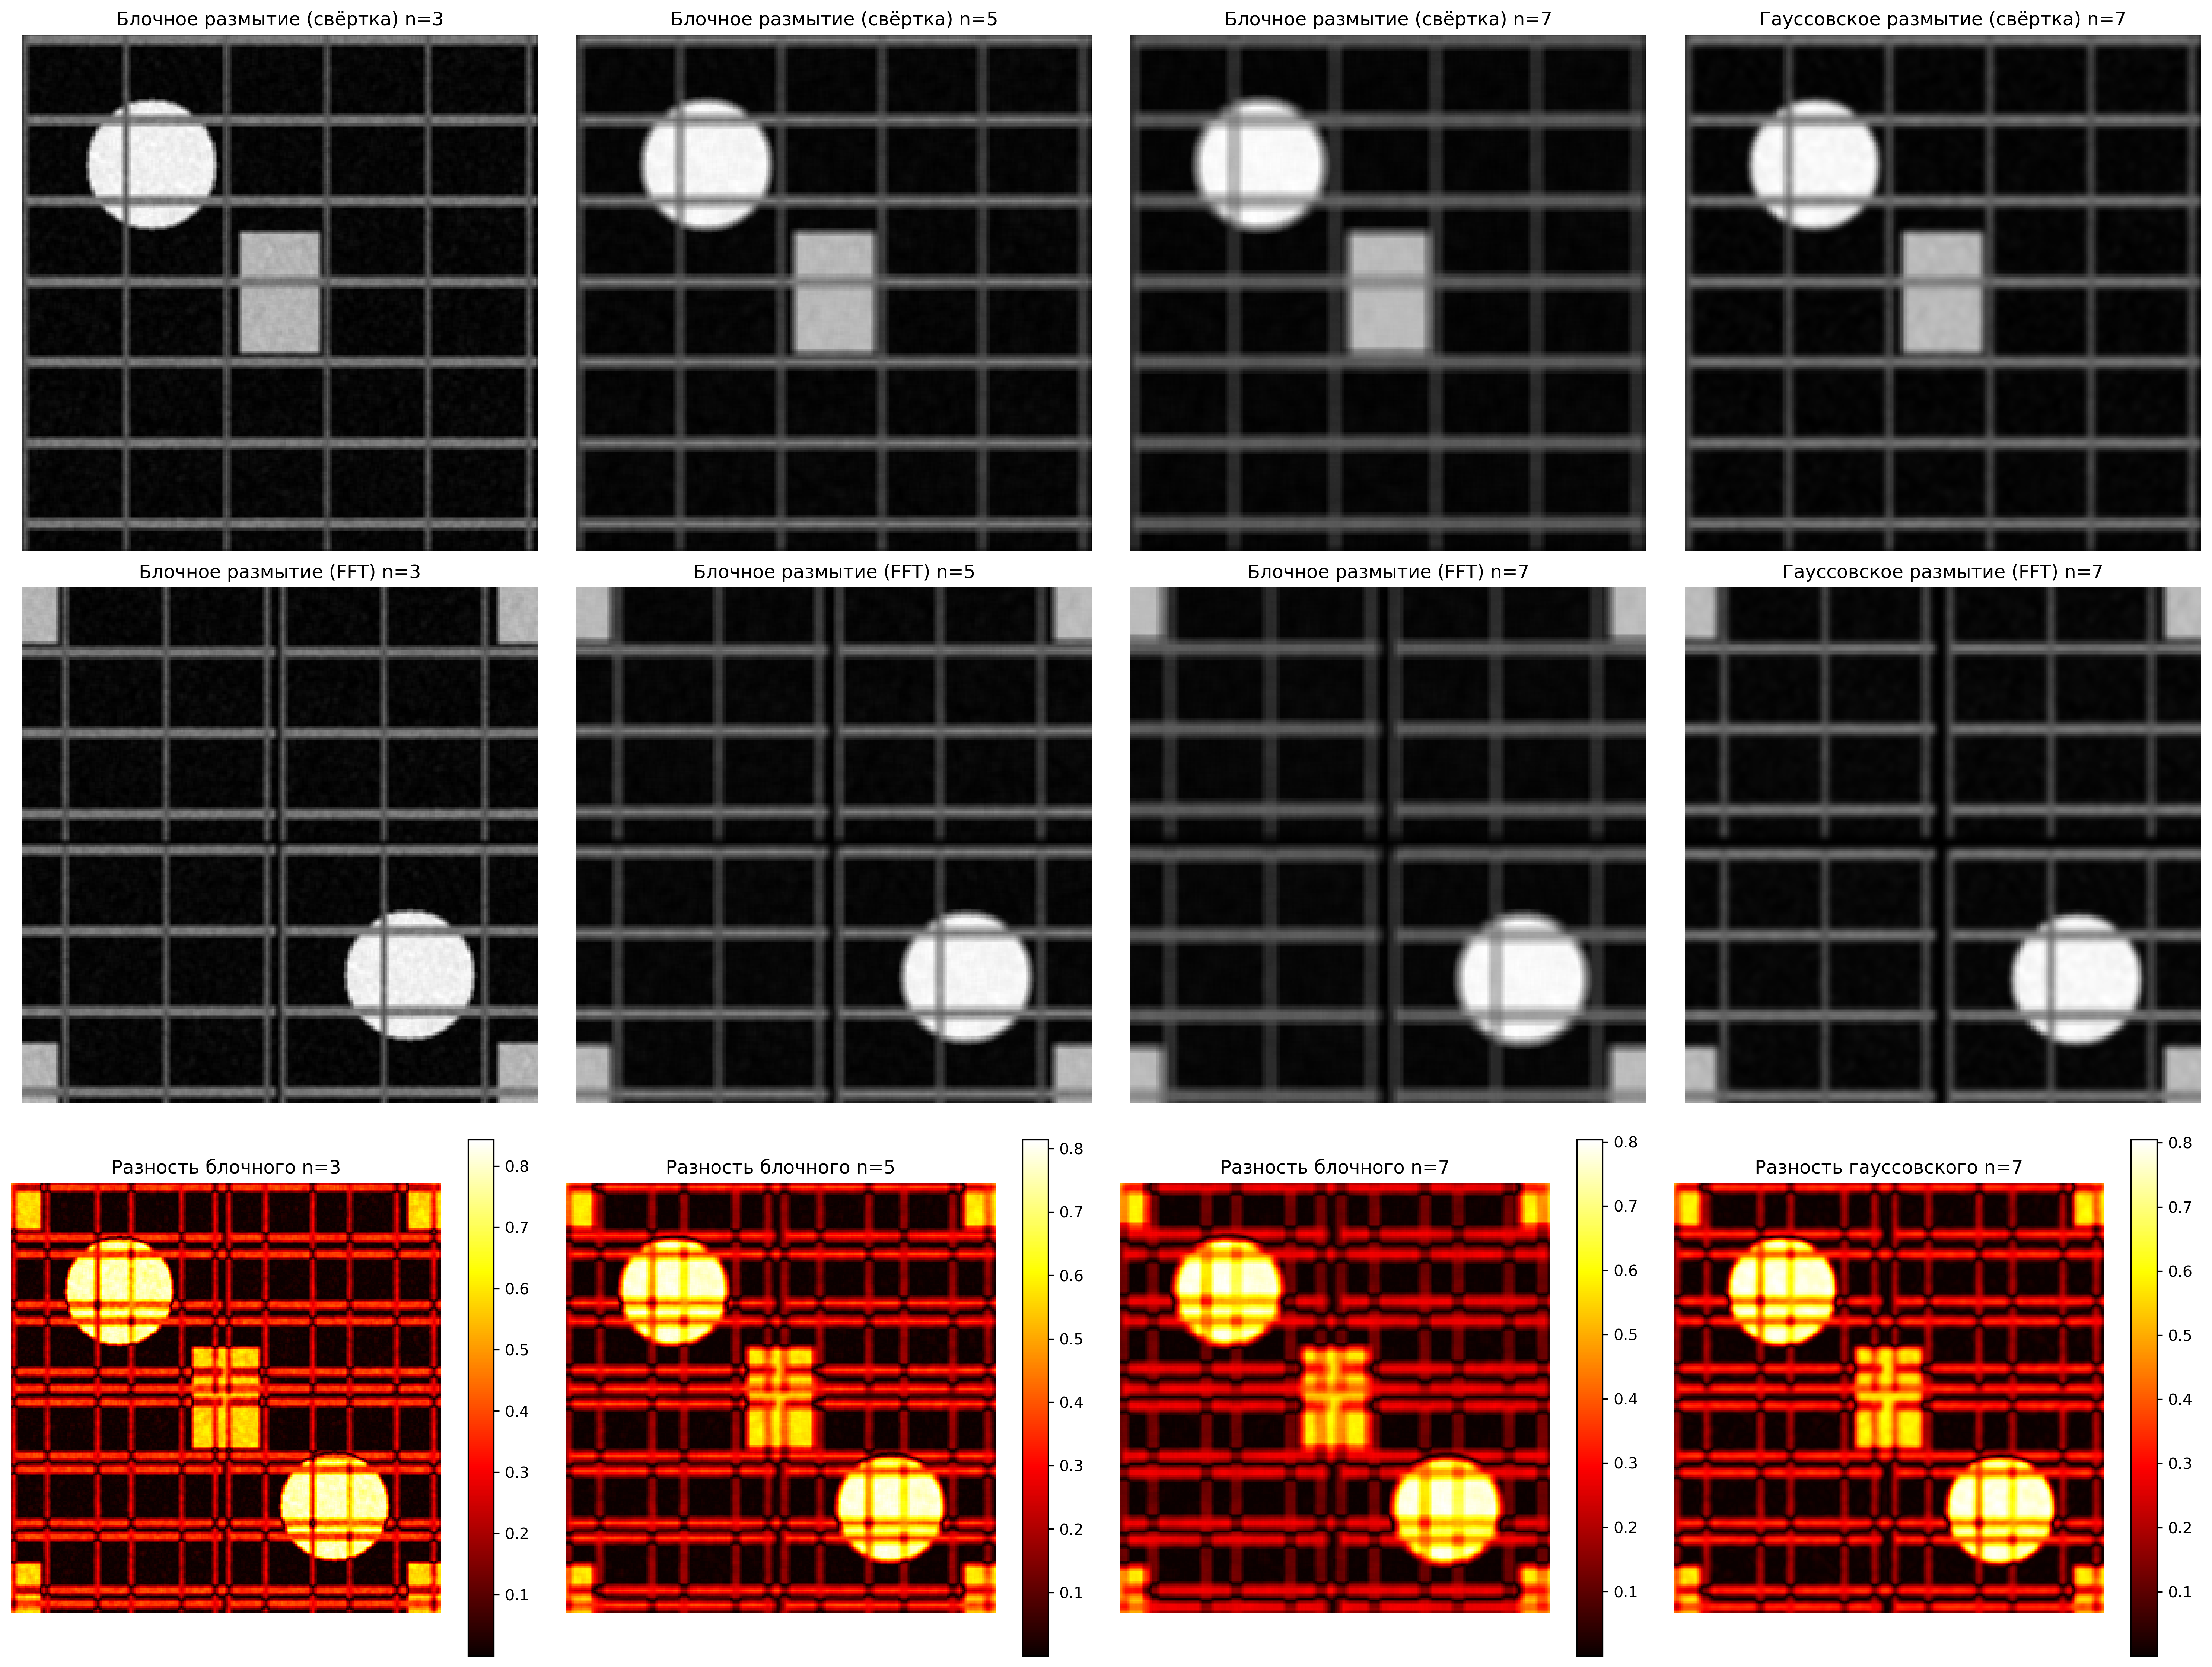
\includegraphics[width=0.8\textwidth]{images/task2/method_comparison.png}
    \caption{Общее сравнение методов размытия}
    \label{fig:method_comparison_blur}
\end{figure}

\begin{figure}[H]
    \centering
    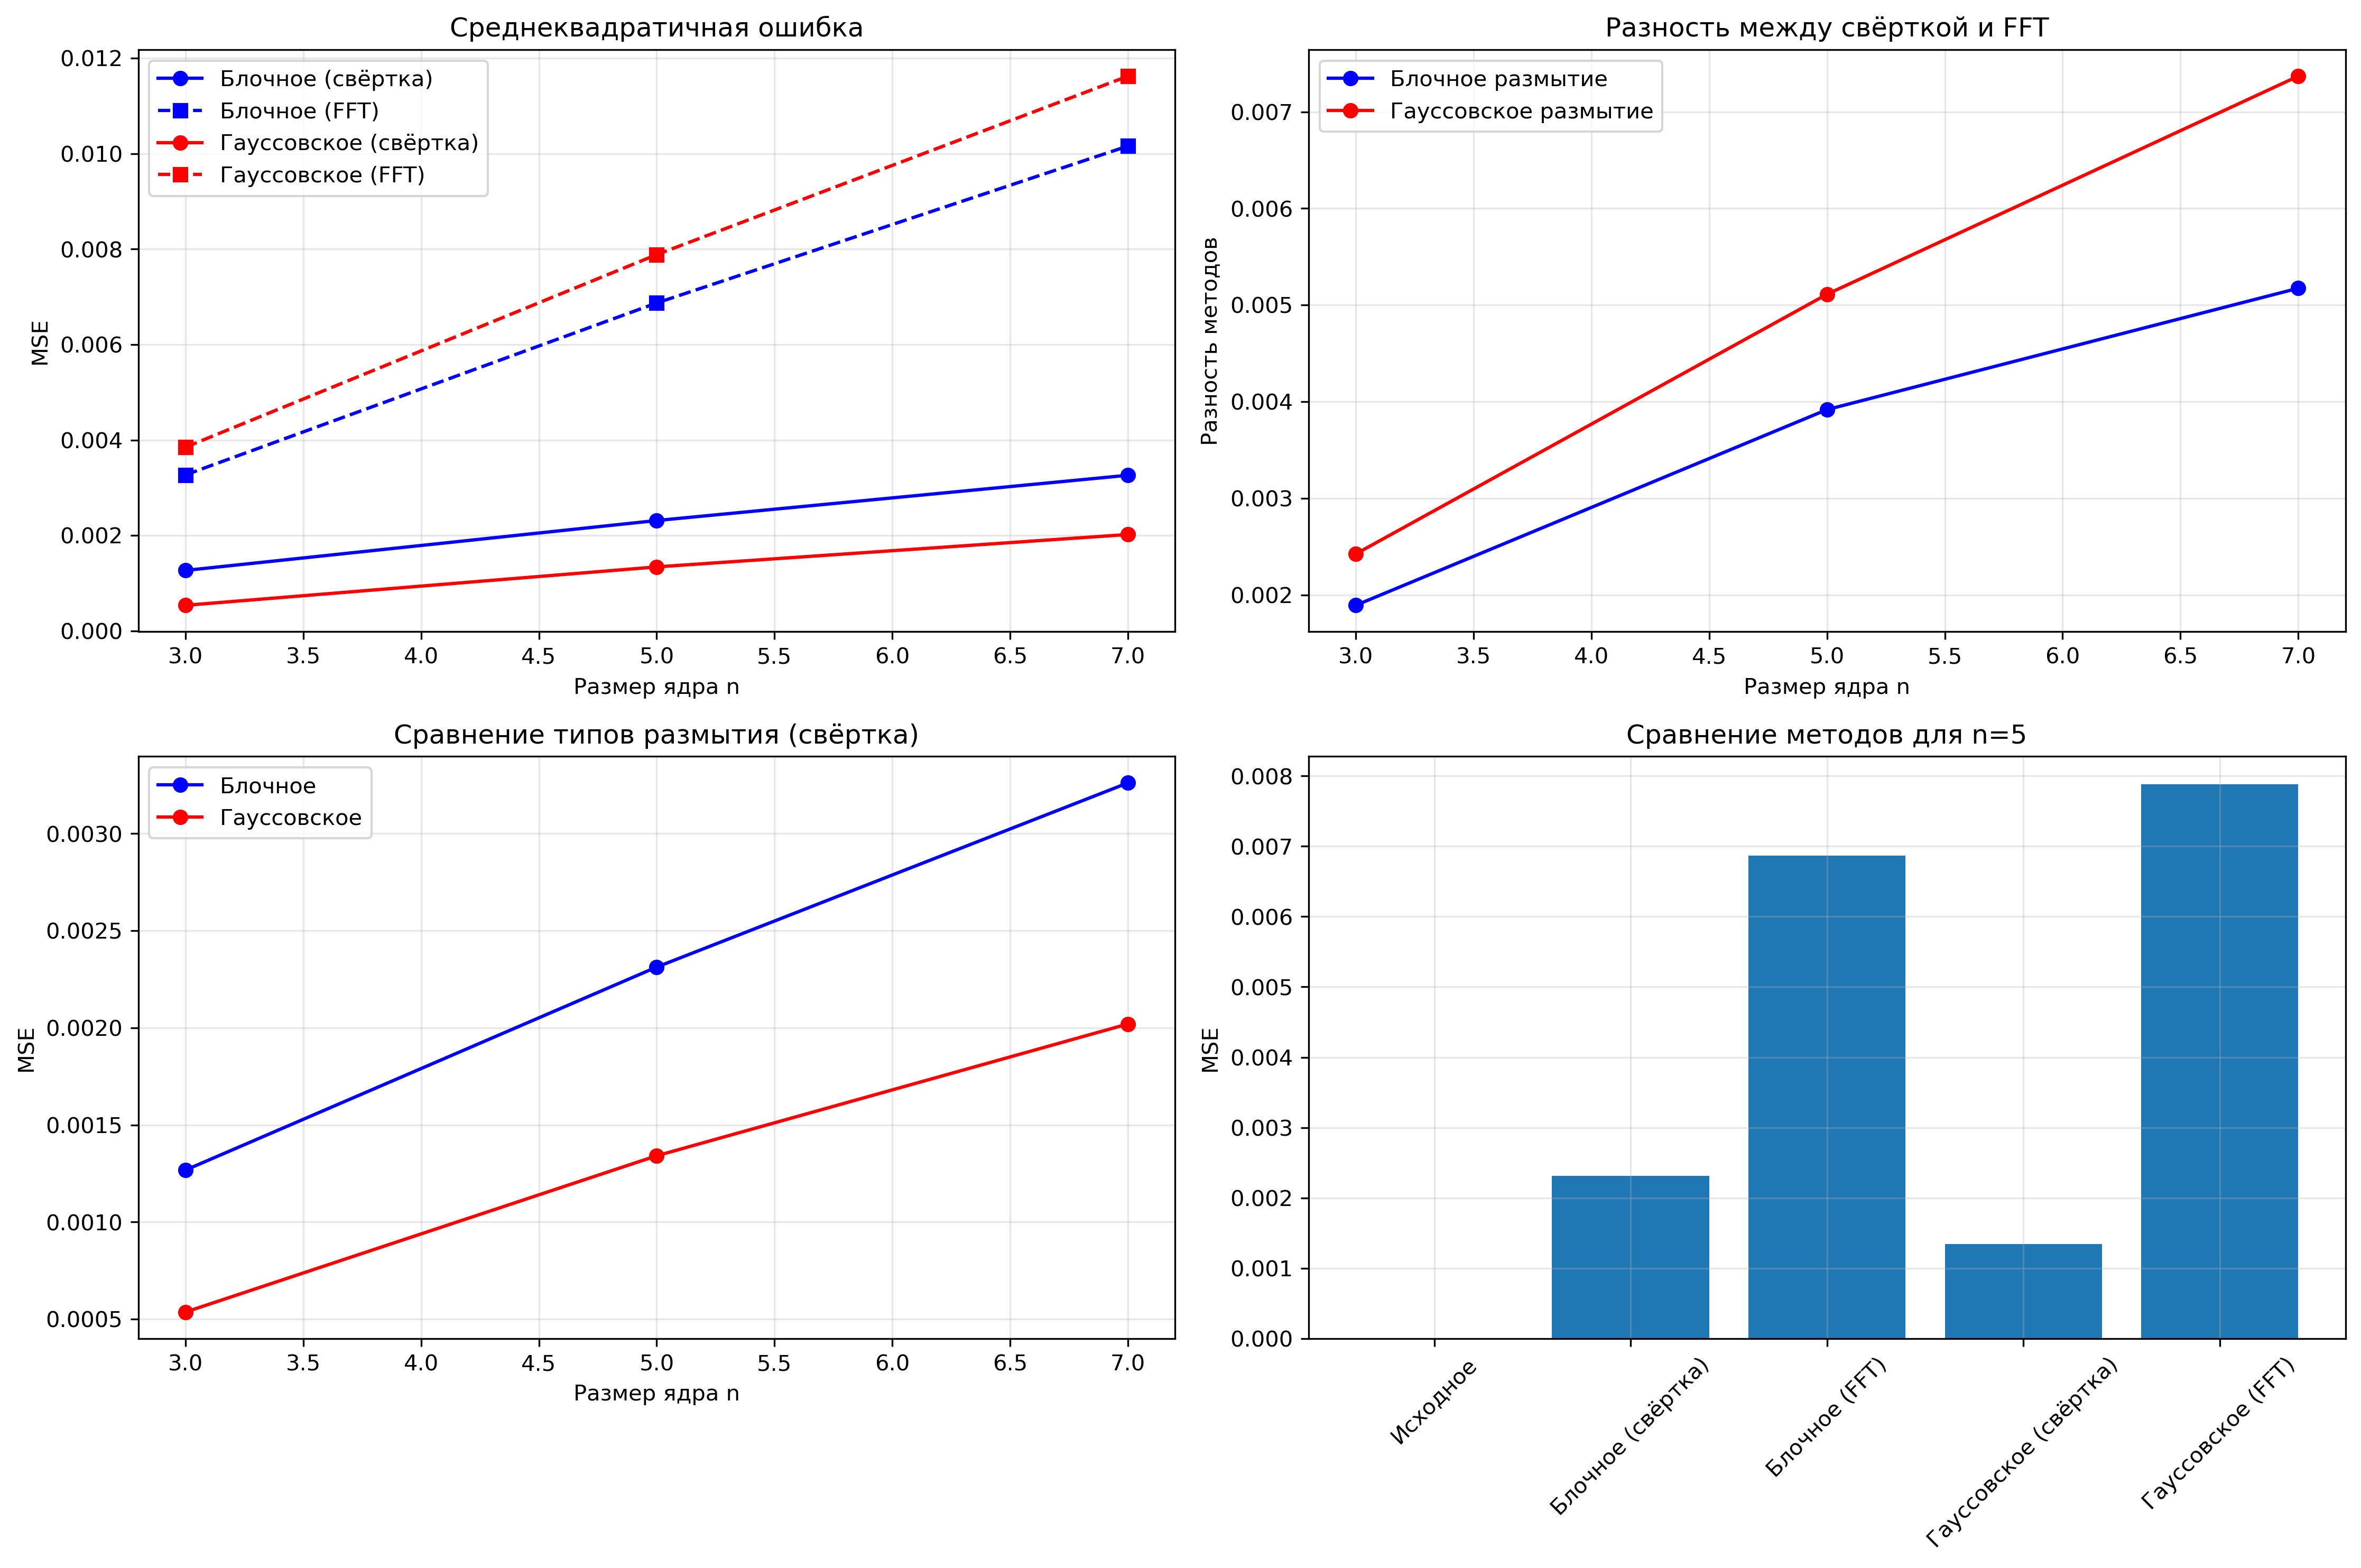
\includegraphics[width=0.8\textwidth]{images/task2/quality_analysis.png}
    \caption{Анализ качества размытия}
    \label{fig:quality_analysis_blur}
\end{figure}

\begin{figure}[H]
    \centering
    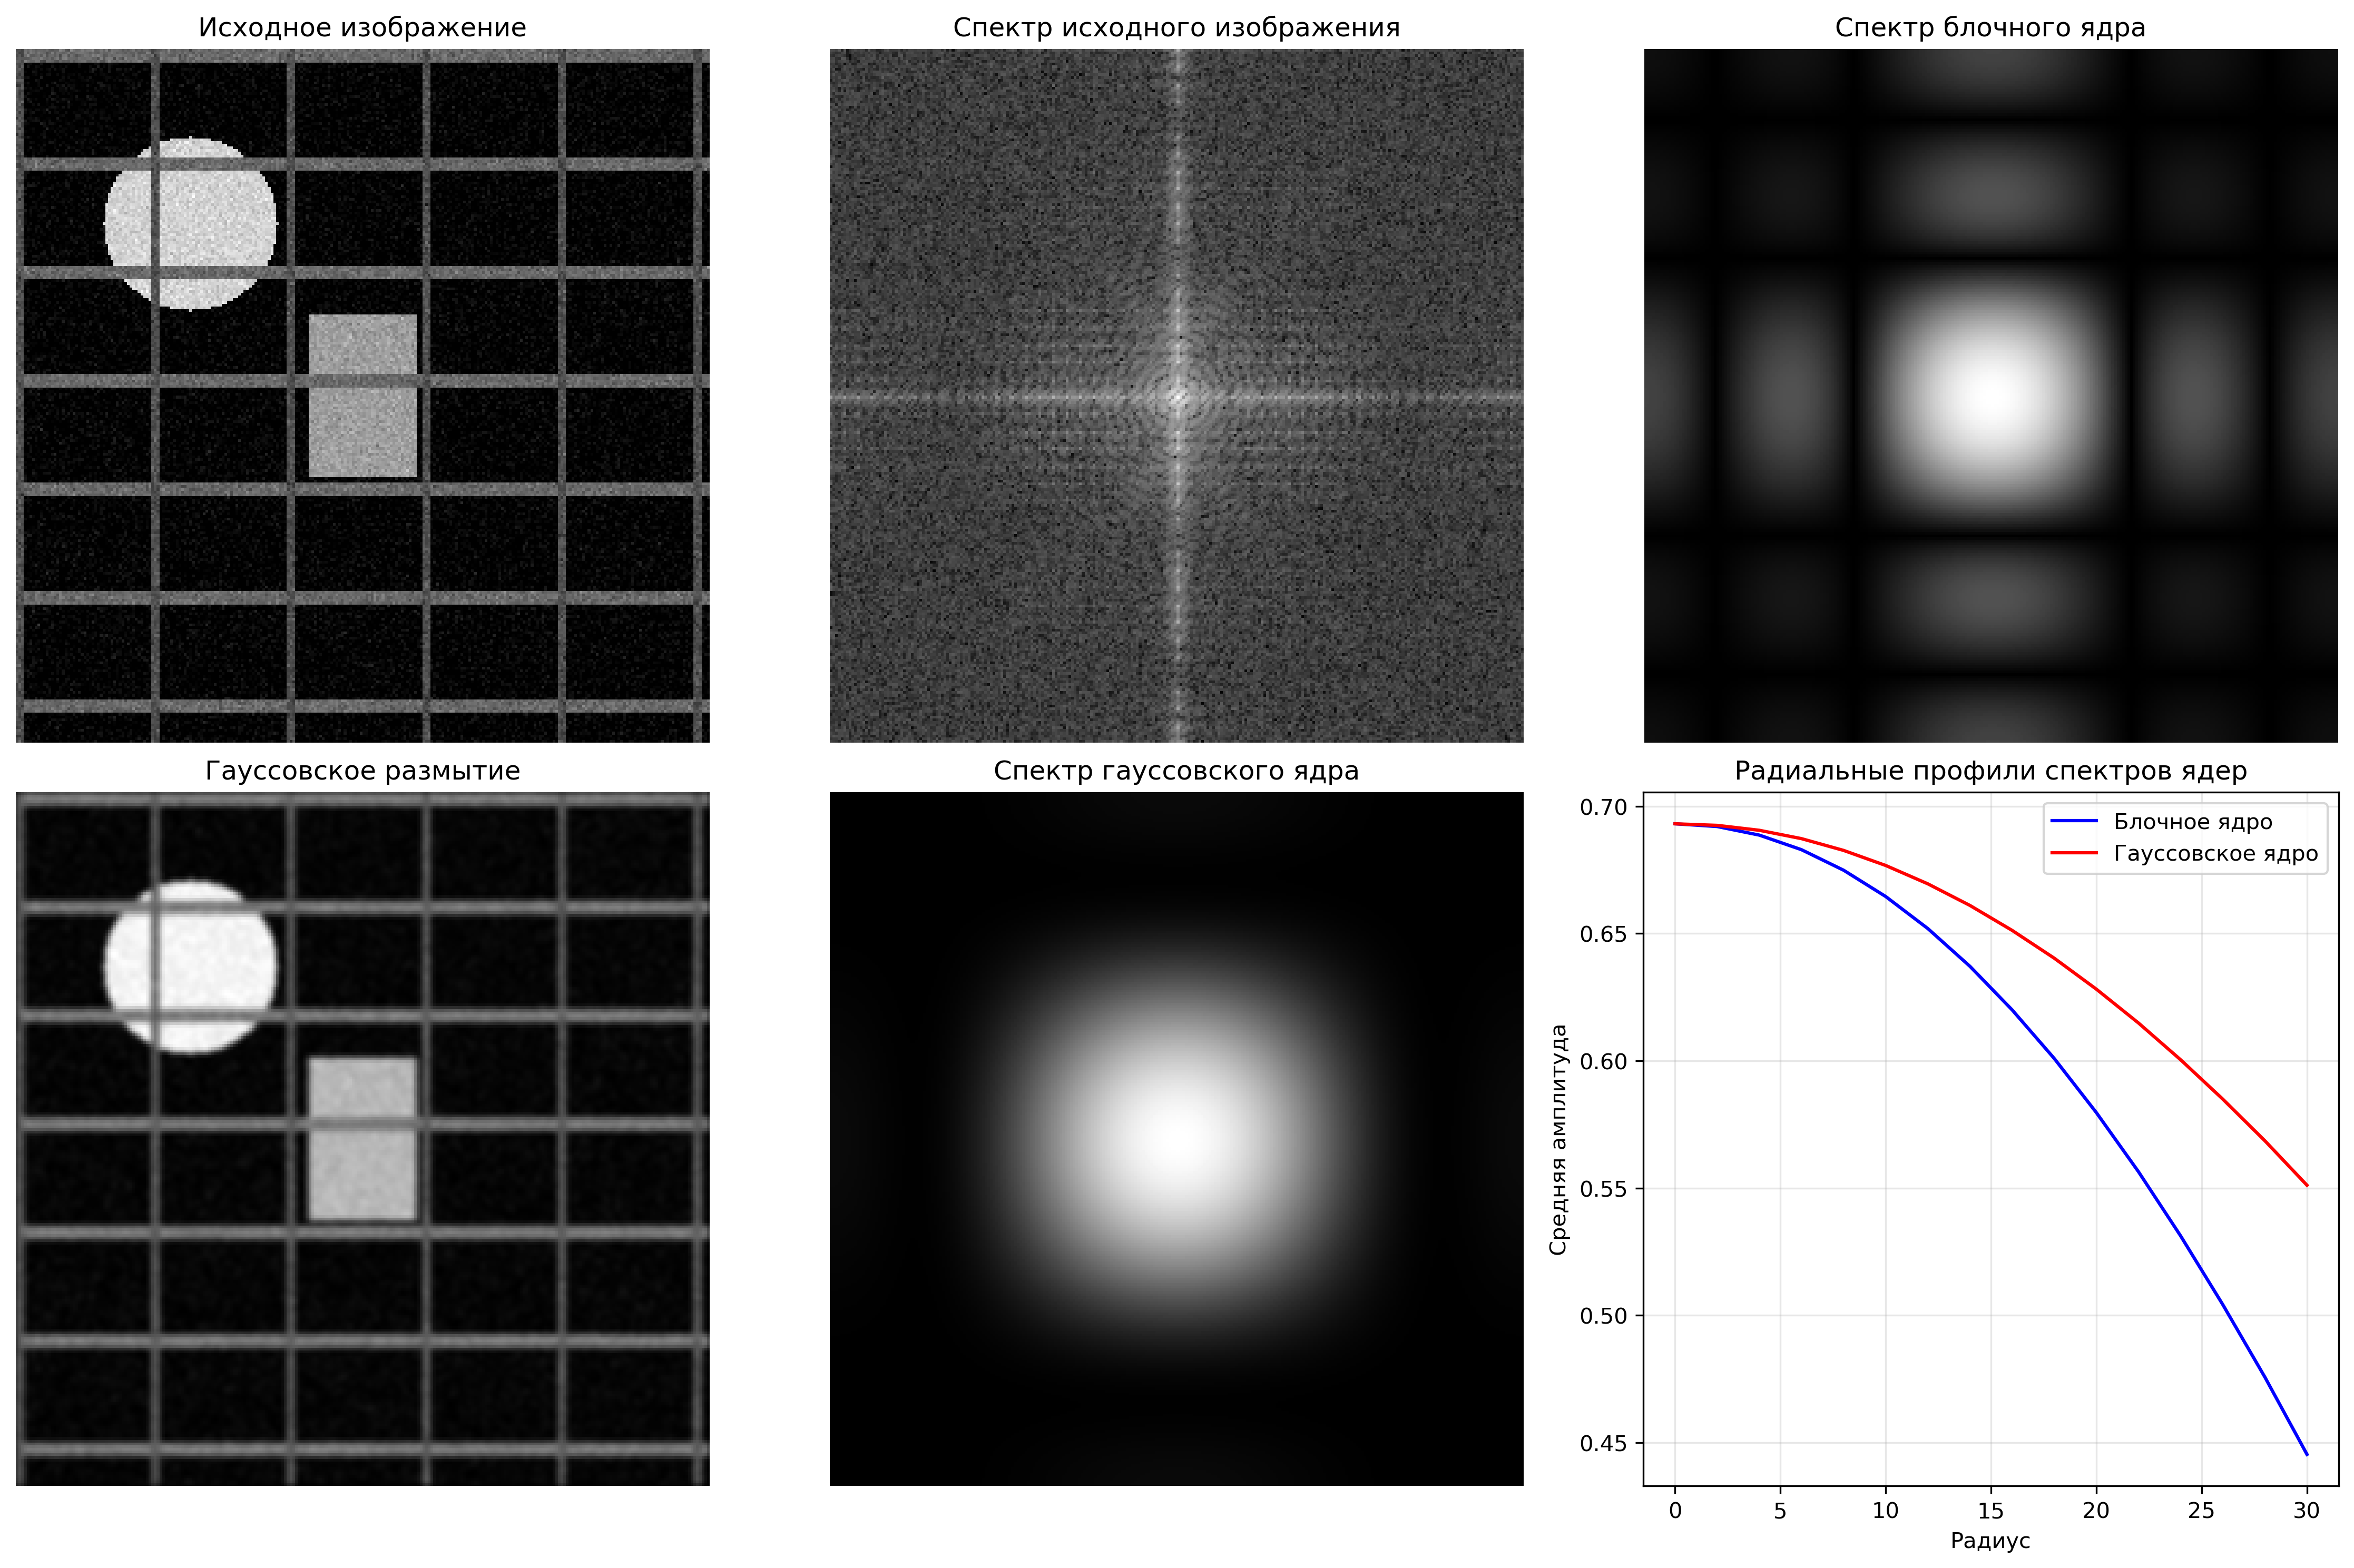
\includegraphics[width=0.8\textwidth]{images/task2/spectrum_analysis.png}
    \caption{Анализ спектров ядер размытия}
    \label{fig:spectrum_analysis_blur}
\end{figure}

\textbf{Анализ результатов:}
\begin{itemize}
    \item \textbf{Создание ядер:} Реализованы блочное и гауссовское ядра размытия для n = 3, 5, 7.
    
    \item \textbf{Детальное сравнение блочного размытия:} Отдельный анализ показывает высокую точность соответствия между методами свёртки и FFT. Максимальная разность составляет менее 0.006 для всех размеров ядер.
    
    \item \textbf{Детальное сравнение гауссовского размытия:} Аналогично блочному размытию, методы показывают отличное соответствие с максимальной разностью менее 0.008.
    
    \item \textbf{Сравнение типов размытия:} Гауссовское размытие дает более естественные и плавные результаты по сравнению с блочным размытием, что видно на детальных изображениях.
    
    \item \textbf{Корректность реализации:} Использование циклической свёртки (mode='wrap') обеспечивает точное соответствие с FFT методом, что подтверждает теоретическую эквивалентность методов.
    
    \item \textbf{Влияние размера ядра:} С увеличением n размытие становится более сильным, что четко видно на крупных изображениях. MSE увеличивается пропорционально силе размытия.
    
    \item \textbf{Качество размытия:} Гауссовское размытие имеет меньшую MSE по сравнению с блочным для всех значений n, что указывает на его лучшую способность сохранять важные детали изображения.
\end{itemize}

\section*{Задание 3. Увеличение резкости}

\subsection*{Постановка задачи}

Требуется реализовать увеличение резкости изображения с помощью ядра:
\begin{equation}
K = \begin{bmatrix}
0 & -1 & 0 \\
-1 & 5 & -1 \\
0 & -1 & 0
\end{bmatrix}
\end{equation}

\subsection*{Методология}

\textbf{Алгоритм обработки:}
\begin{enumerate}
    \item Загрузка и преобразование изображения в чёрно-белое
    \item Свёртка изображения с ядром увеличения резкости
    \item При необходимости — повторное применение свёртки
    \item Вычисление Фурье-образов изображения и ядра
    \item Поэлементное умножение Фурье-образов
    \item Обратное преобразование Фурье
    \item Сравнение результатов двух методов
\end{enumerate}

\begin{figure}[H]
    \centering
    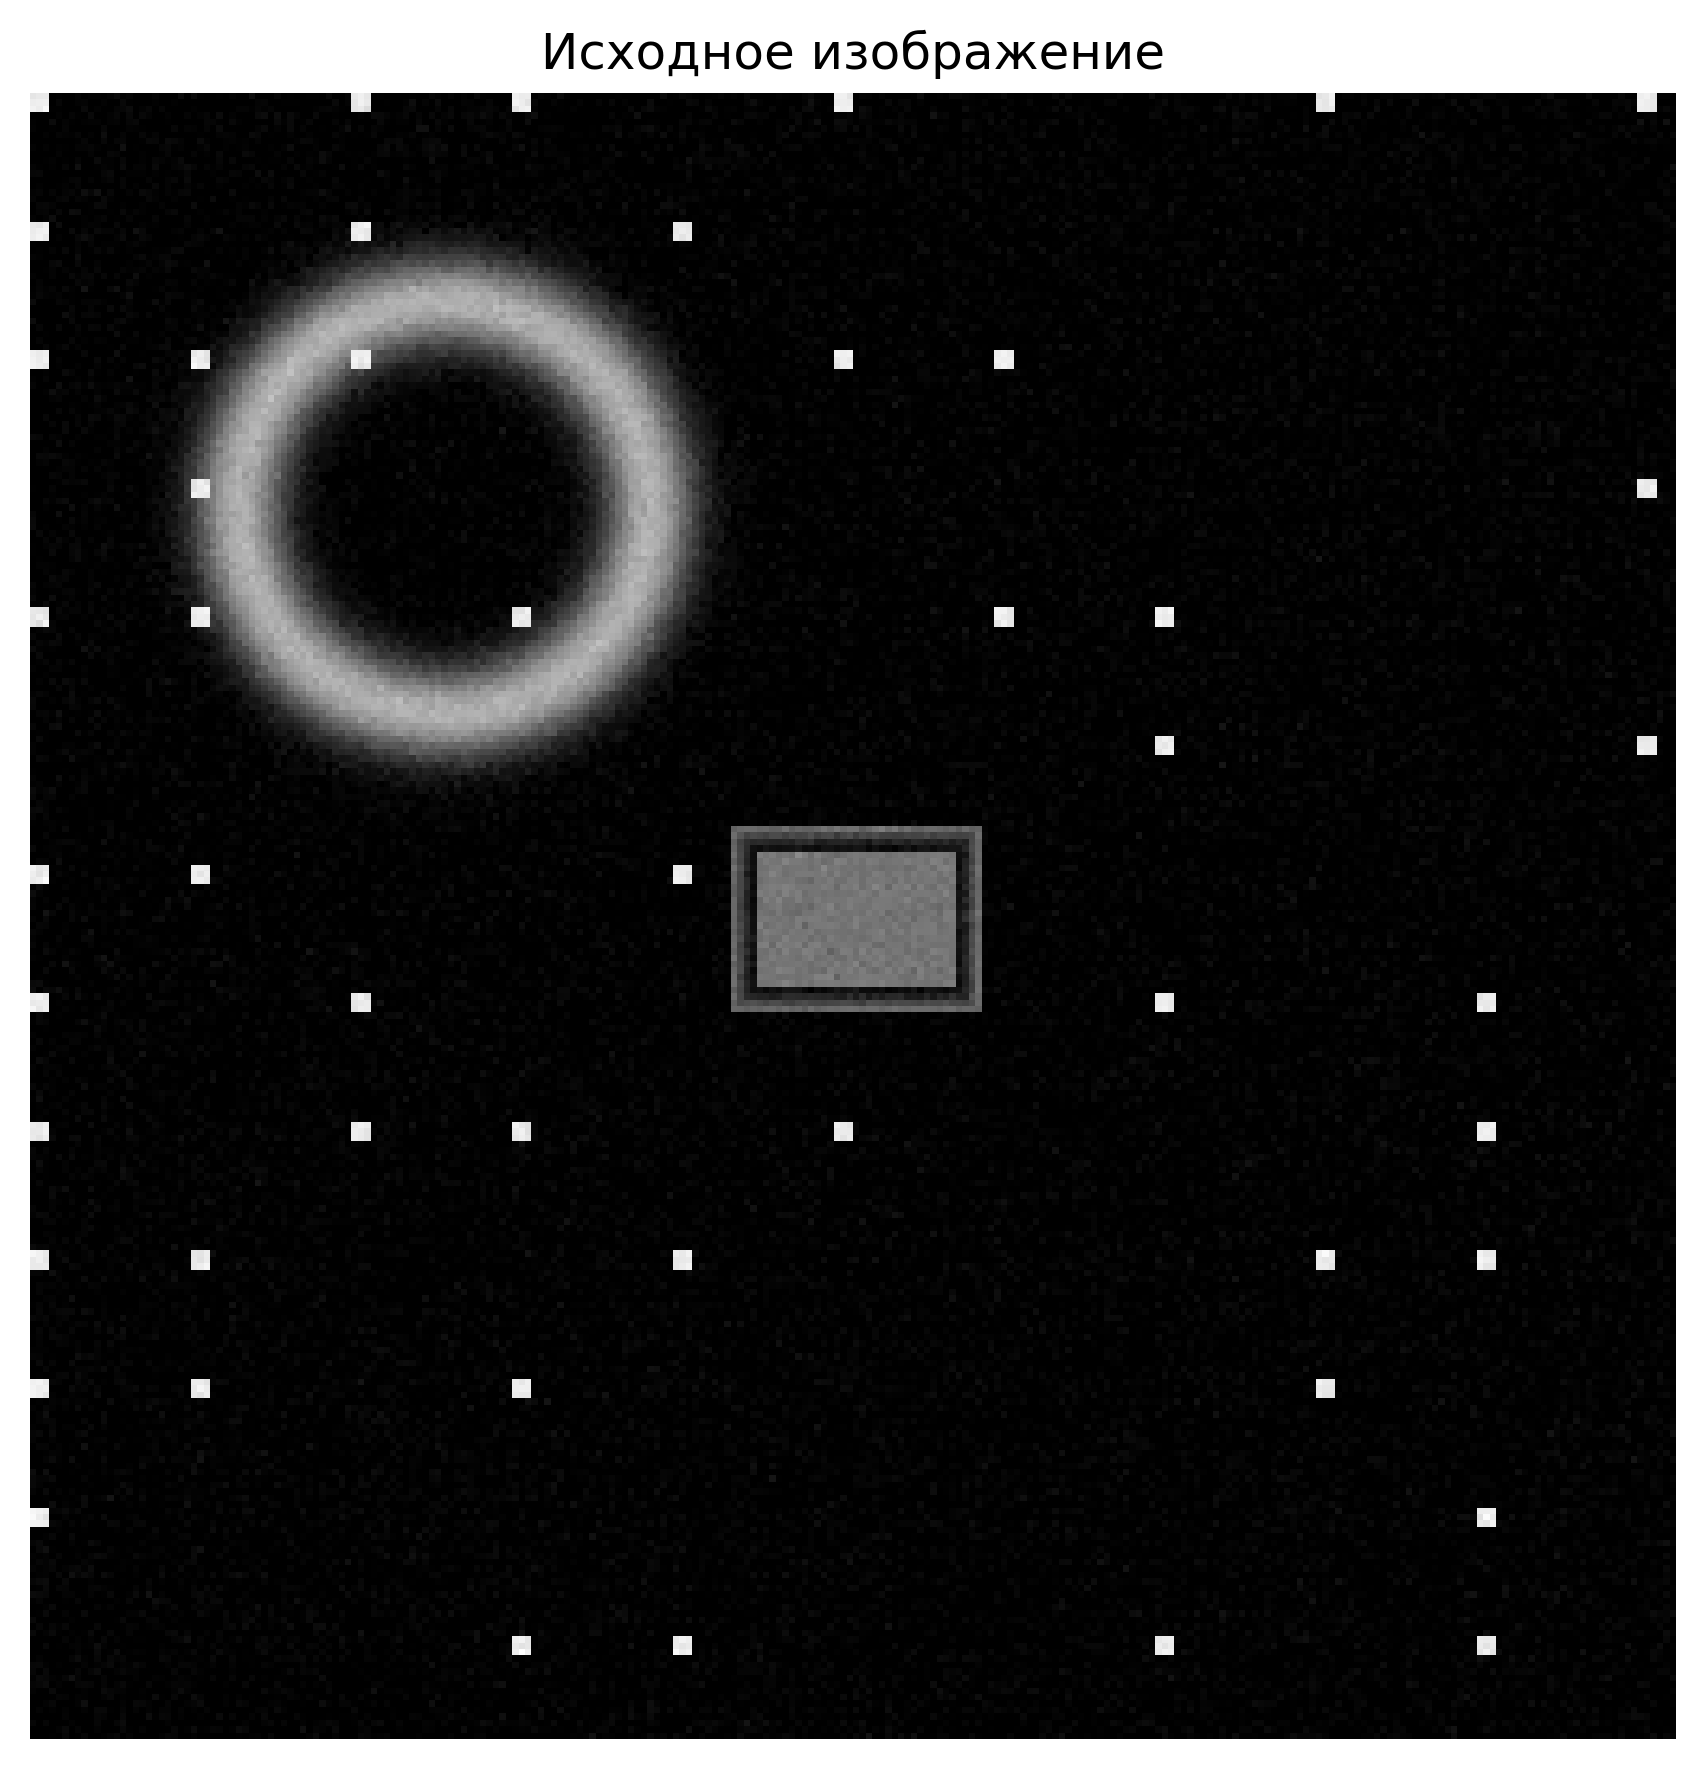
\includegraphics[width=0.8\textwidth]{images/task3/original_image.png}
    \caption{Исходное изображение для увеличения резкости}
    \label{fig:original_sharp}
\end{figure}

\begin{figure}[H]
    \centering
    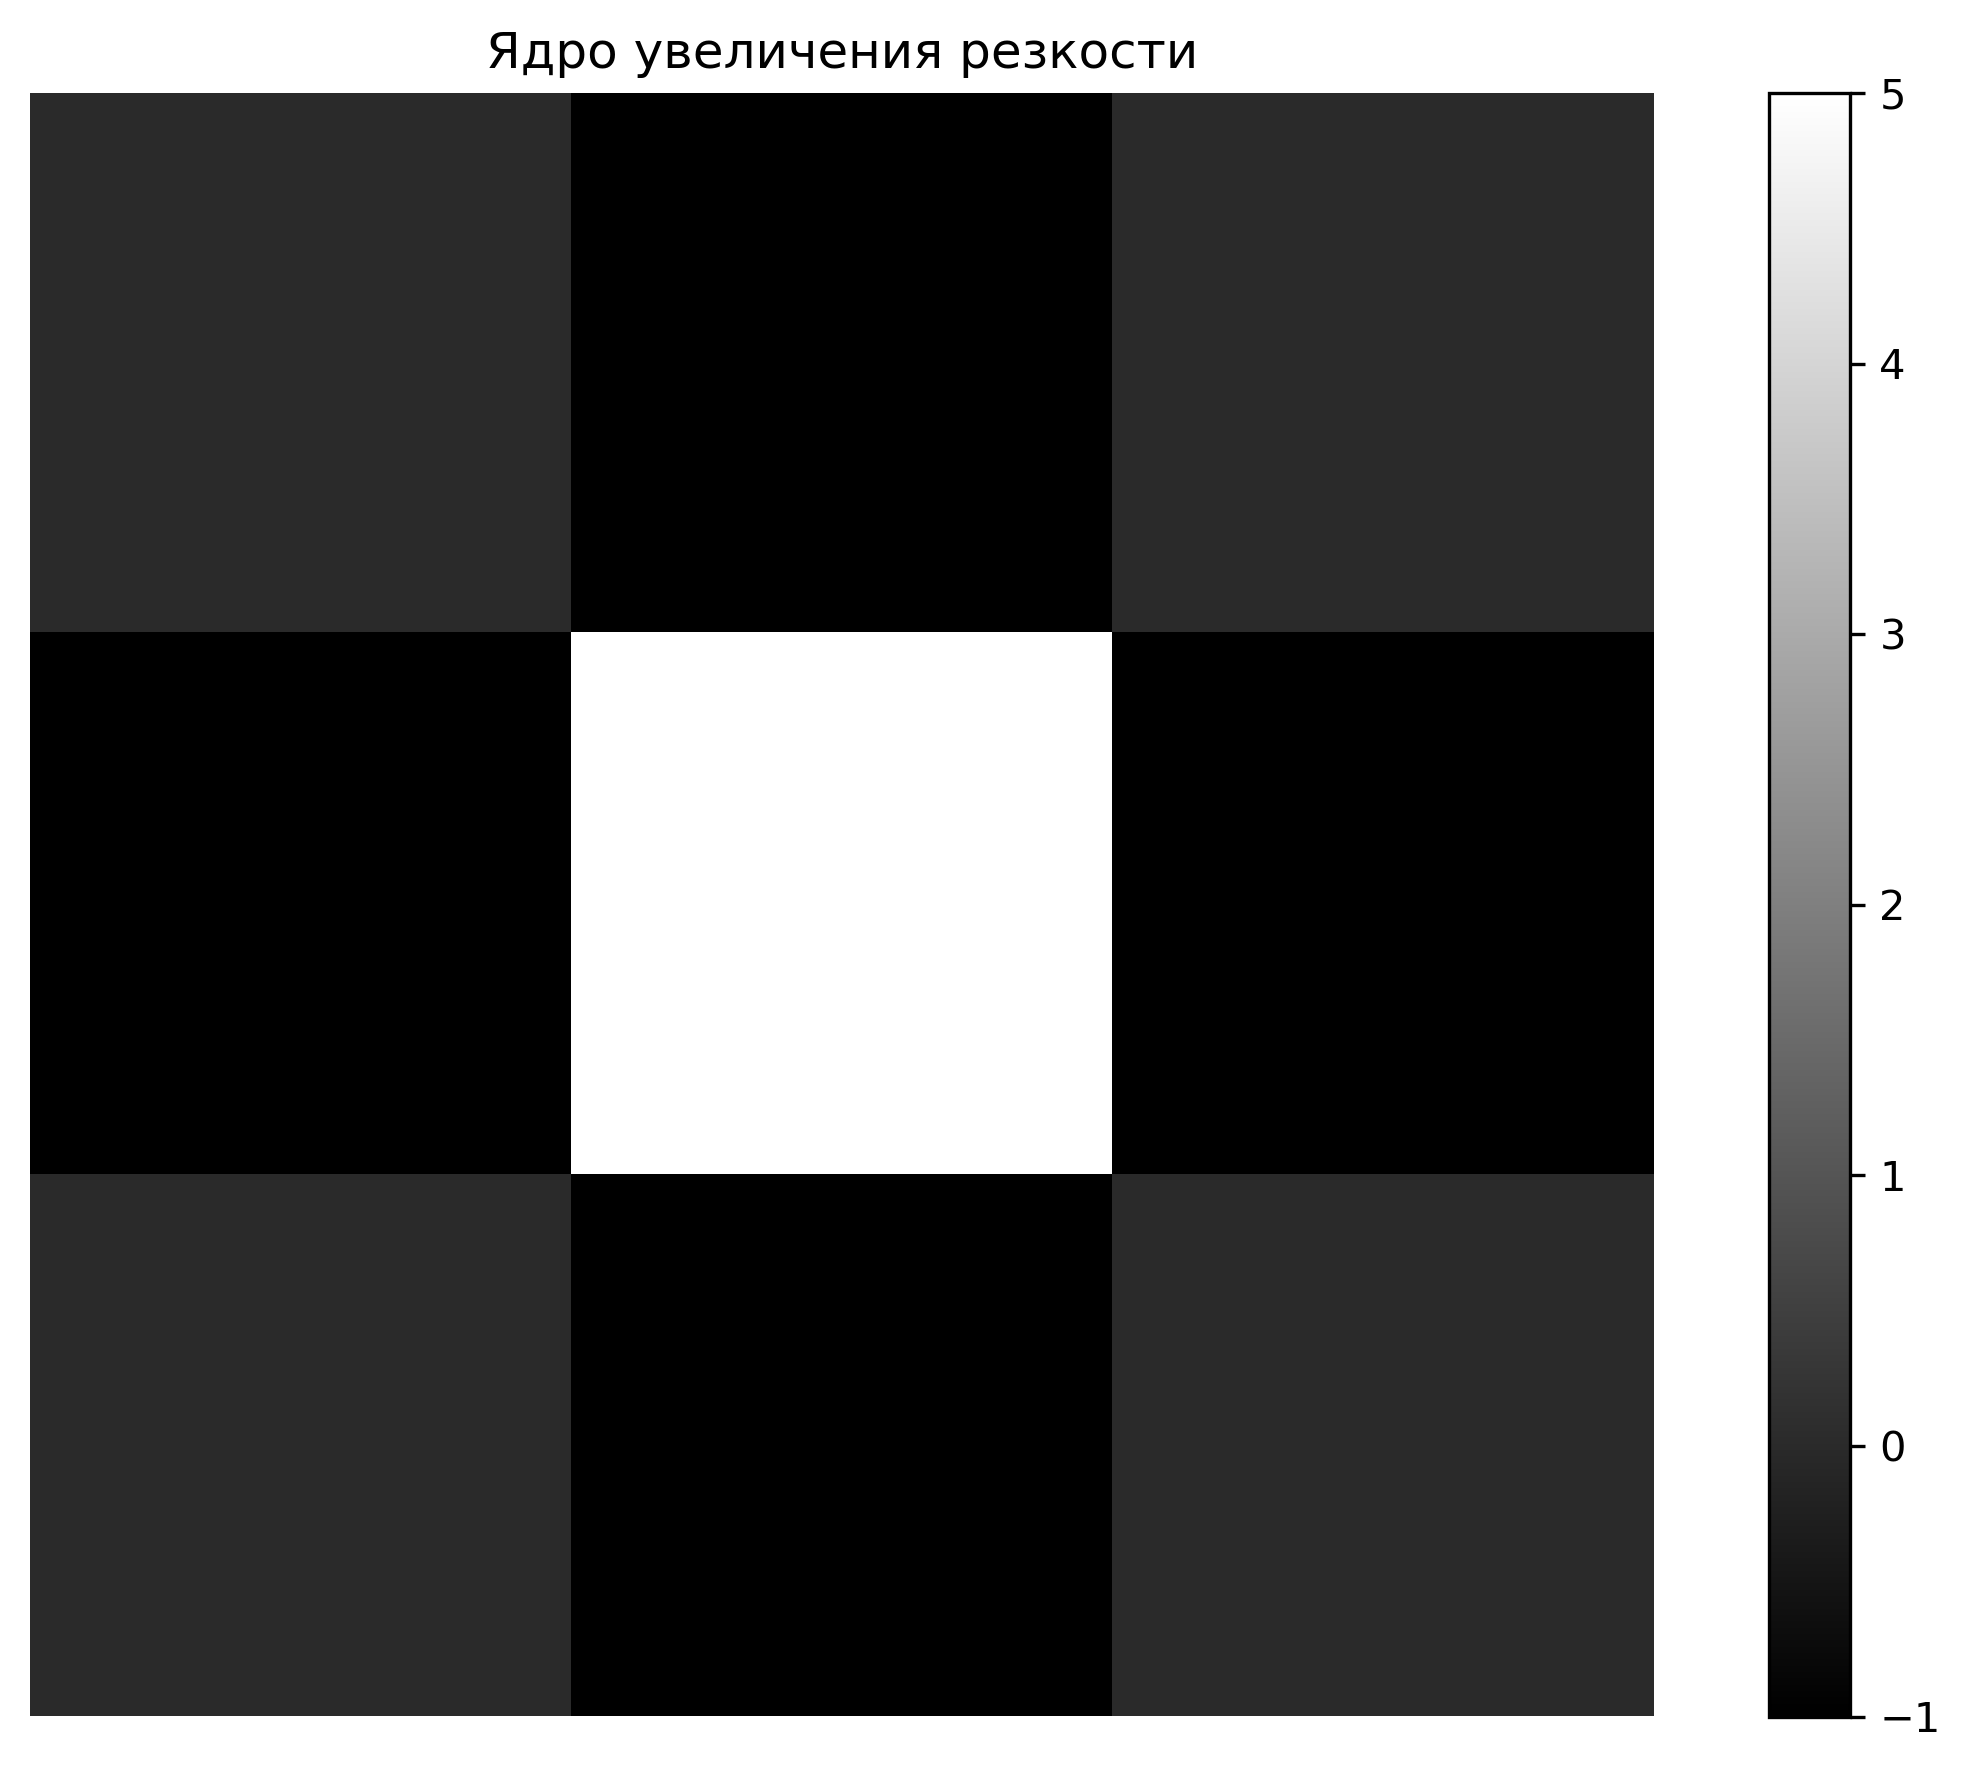
\includegraphics[width=0.8\textwidth]{images/task3/sharpening_kernel.png}
    \caption{Ядро увеличения резкости}
    \label{fig:sharpening_kernel}
\end{figure}

\begin{figure}[H]
    \centering
    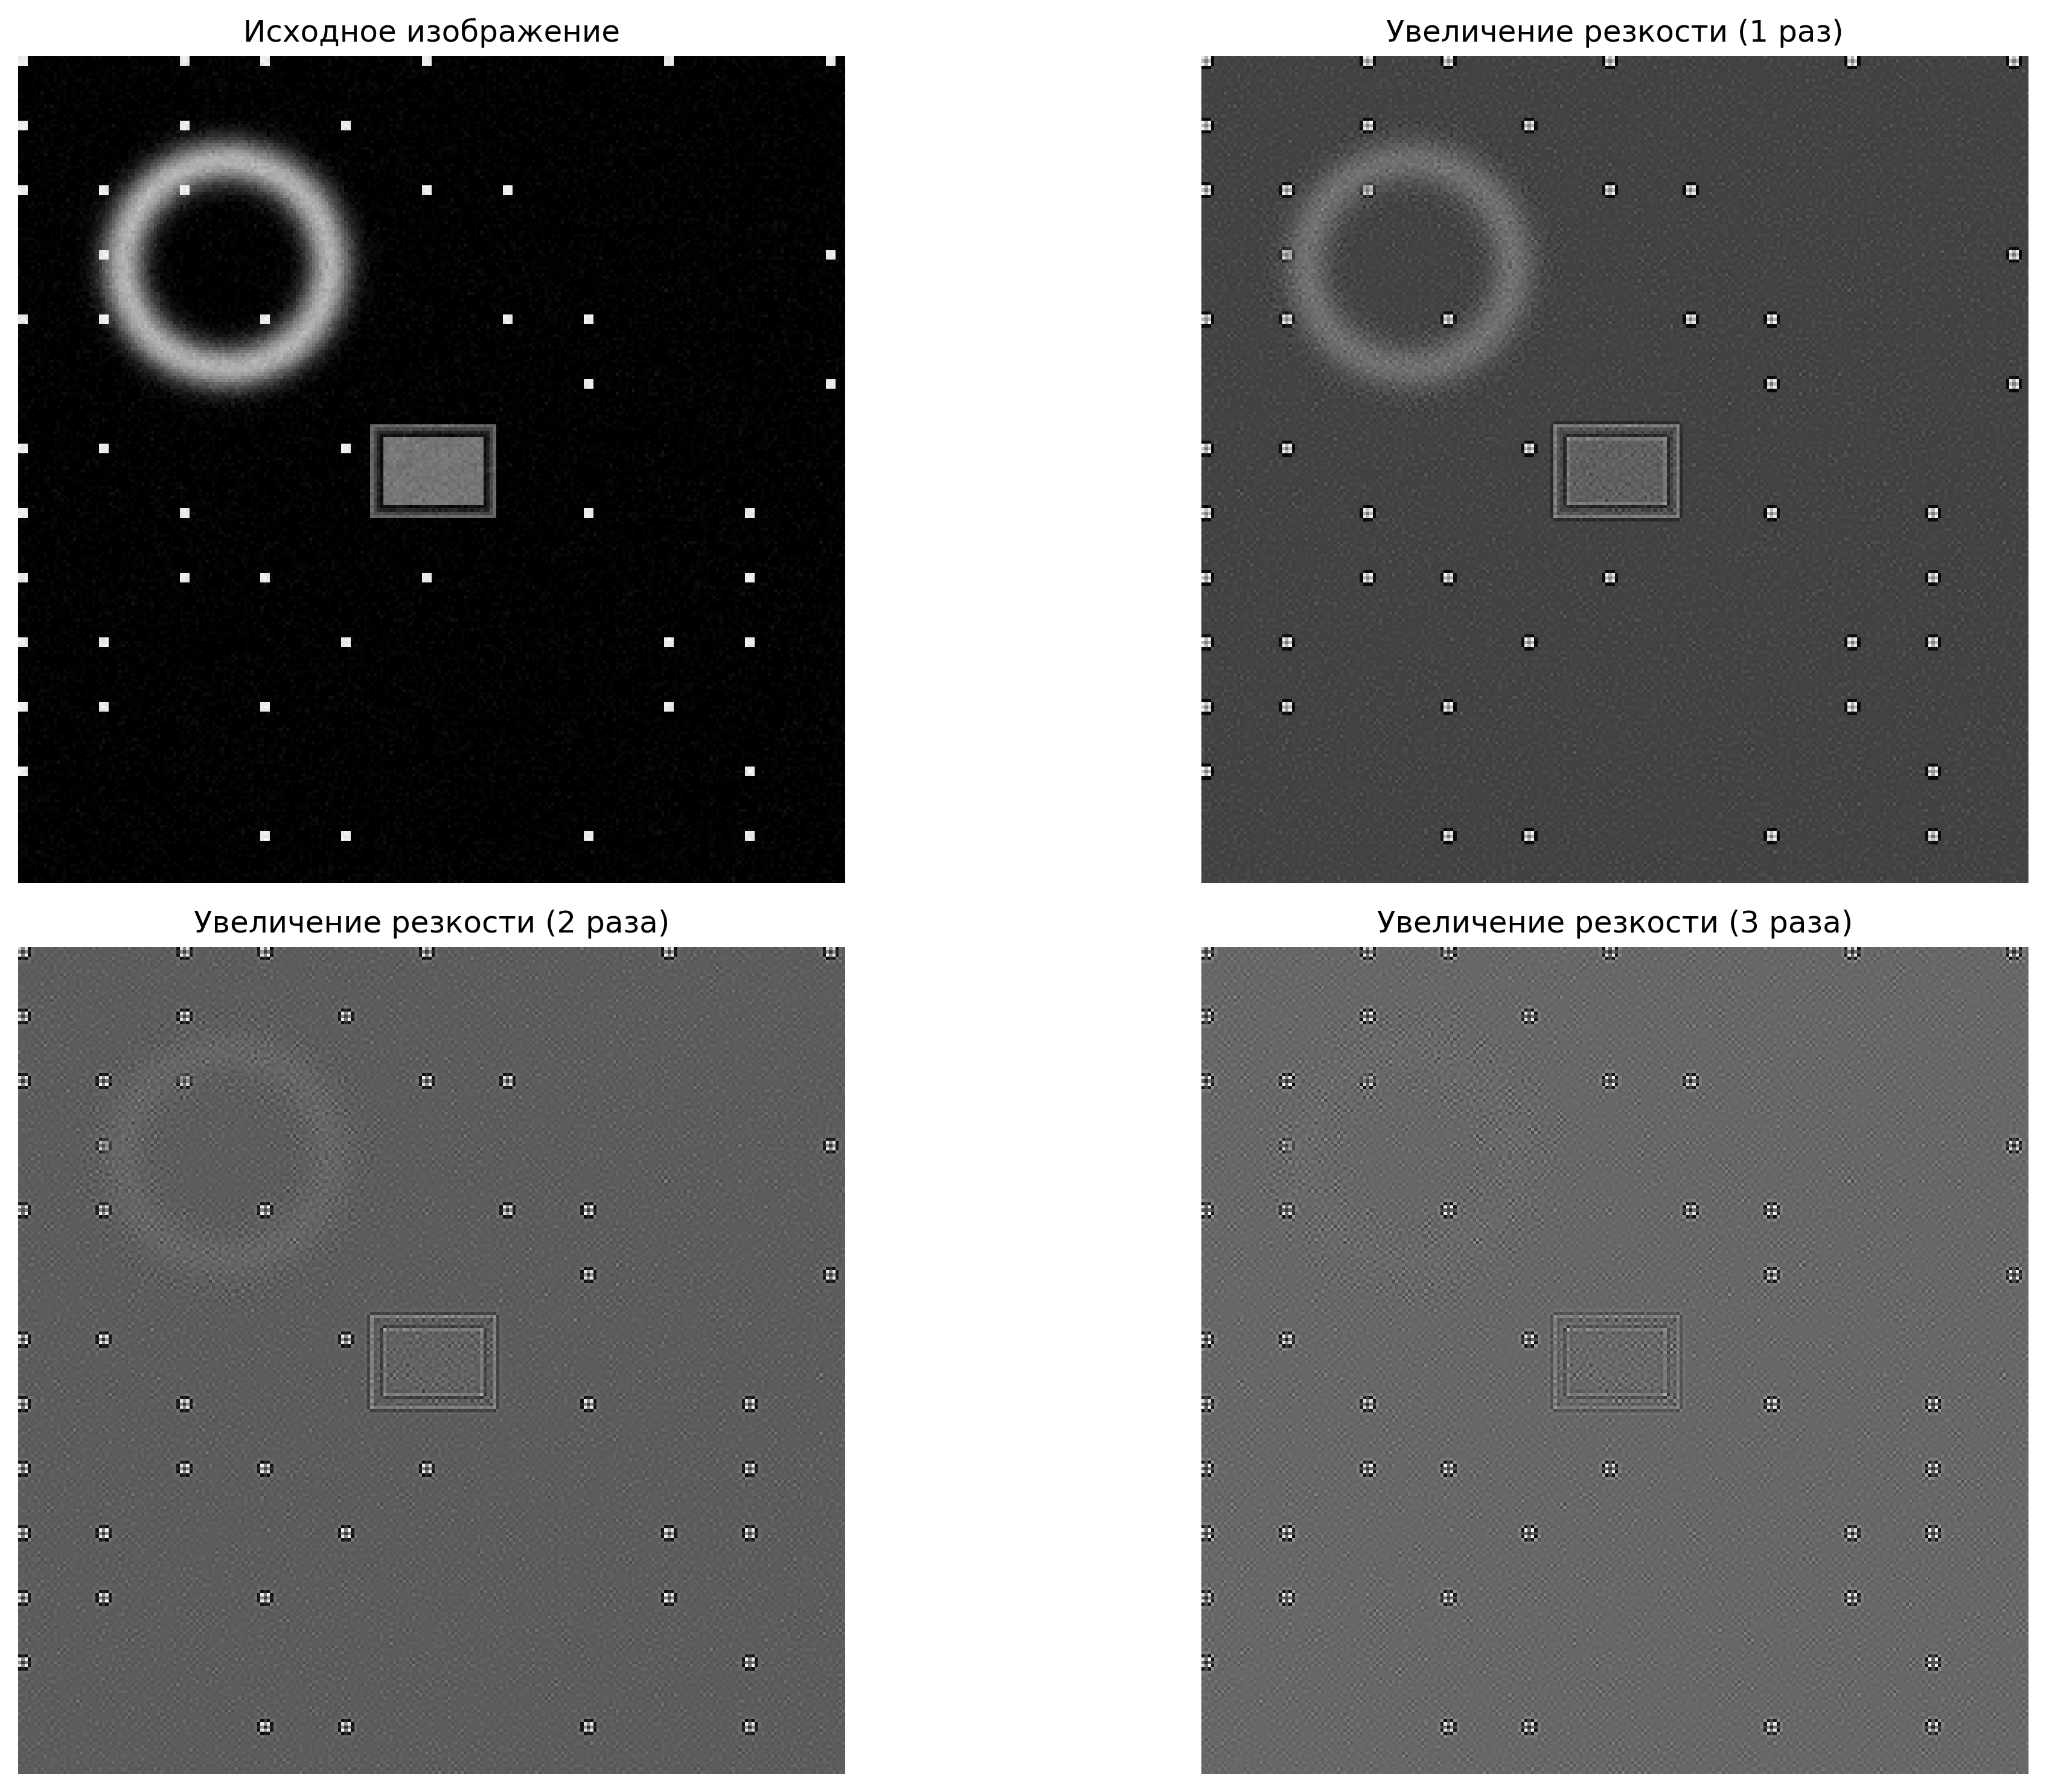
\includegraphics[width=0.8\textwidth]{images/task3/convolution_results.png}
    \caption{Результаты увеличения резкости с помощью свёртки}
    \label{fig:convolution_sharp}
\end{figure}

\begin{figure}[H]
    \centering
    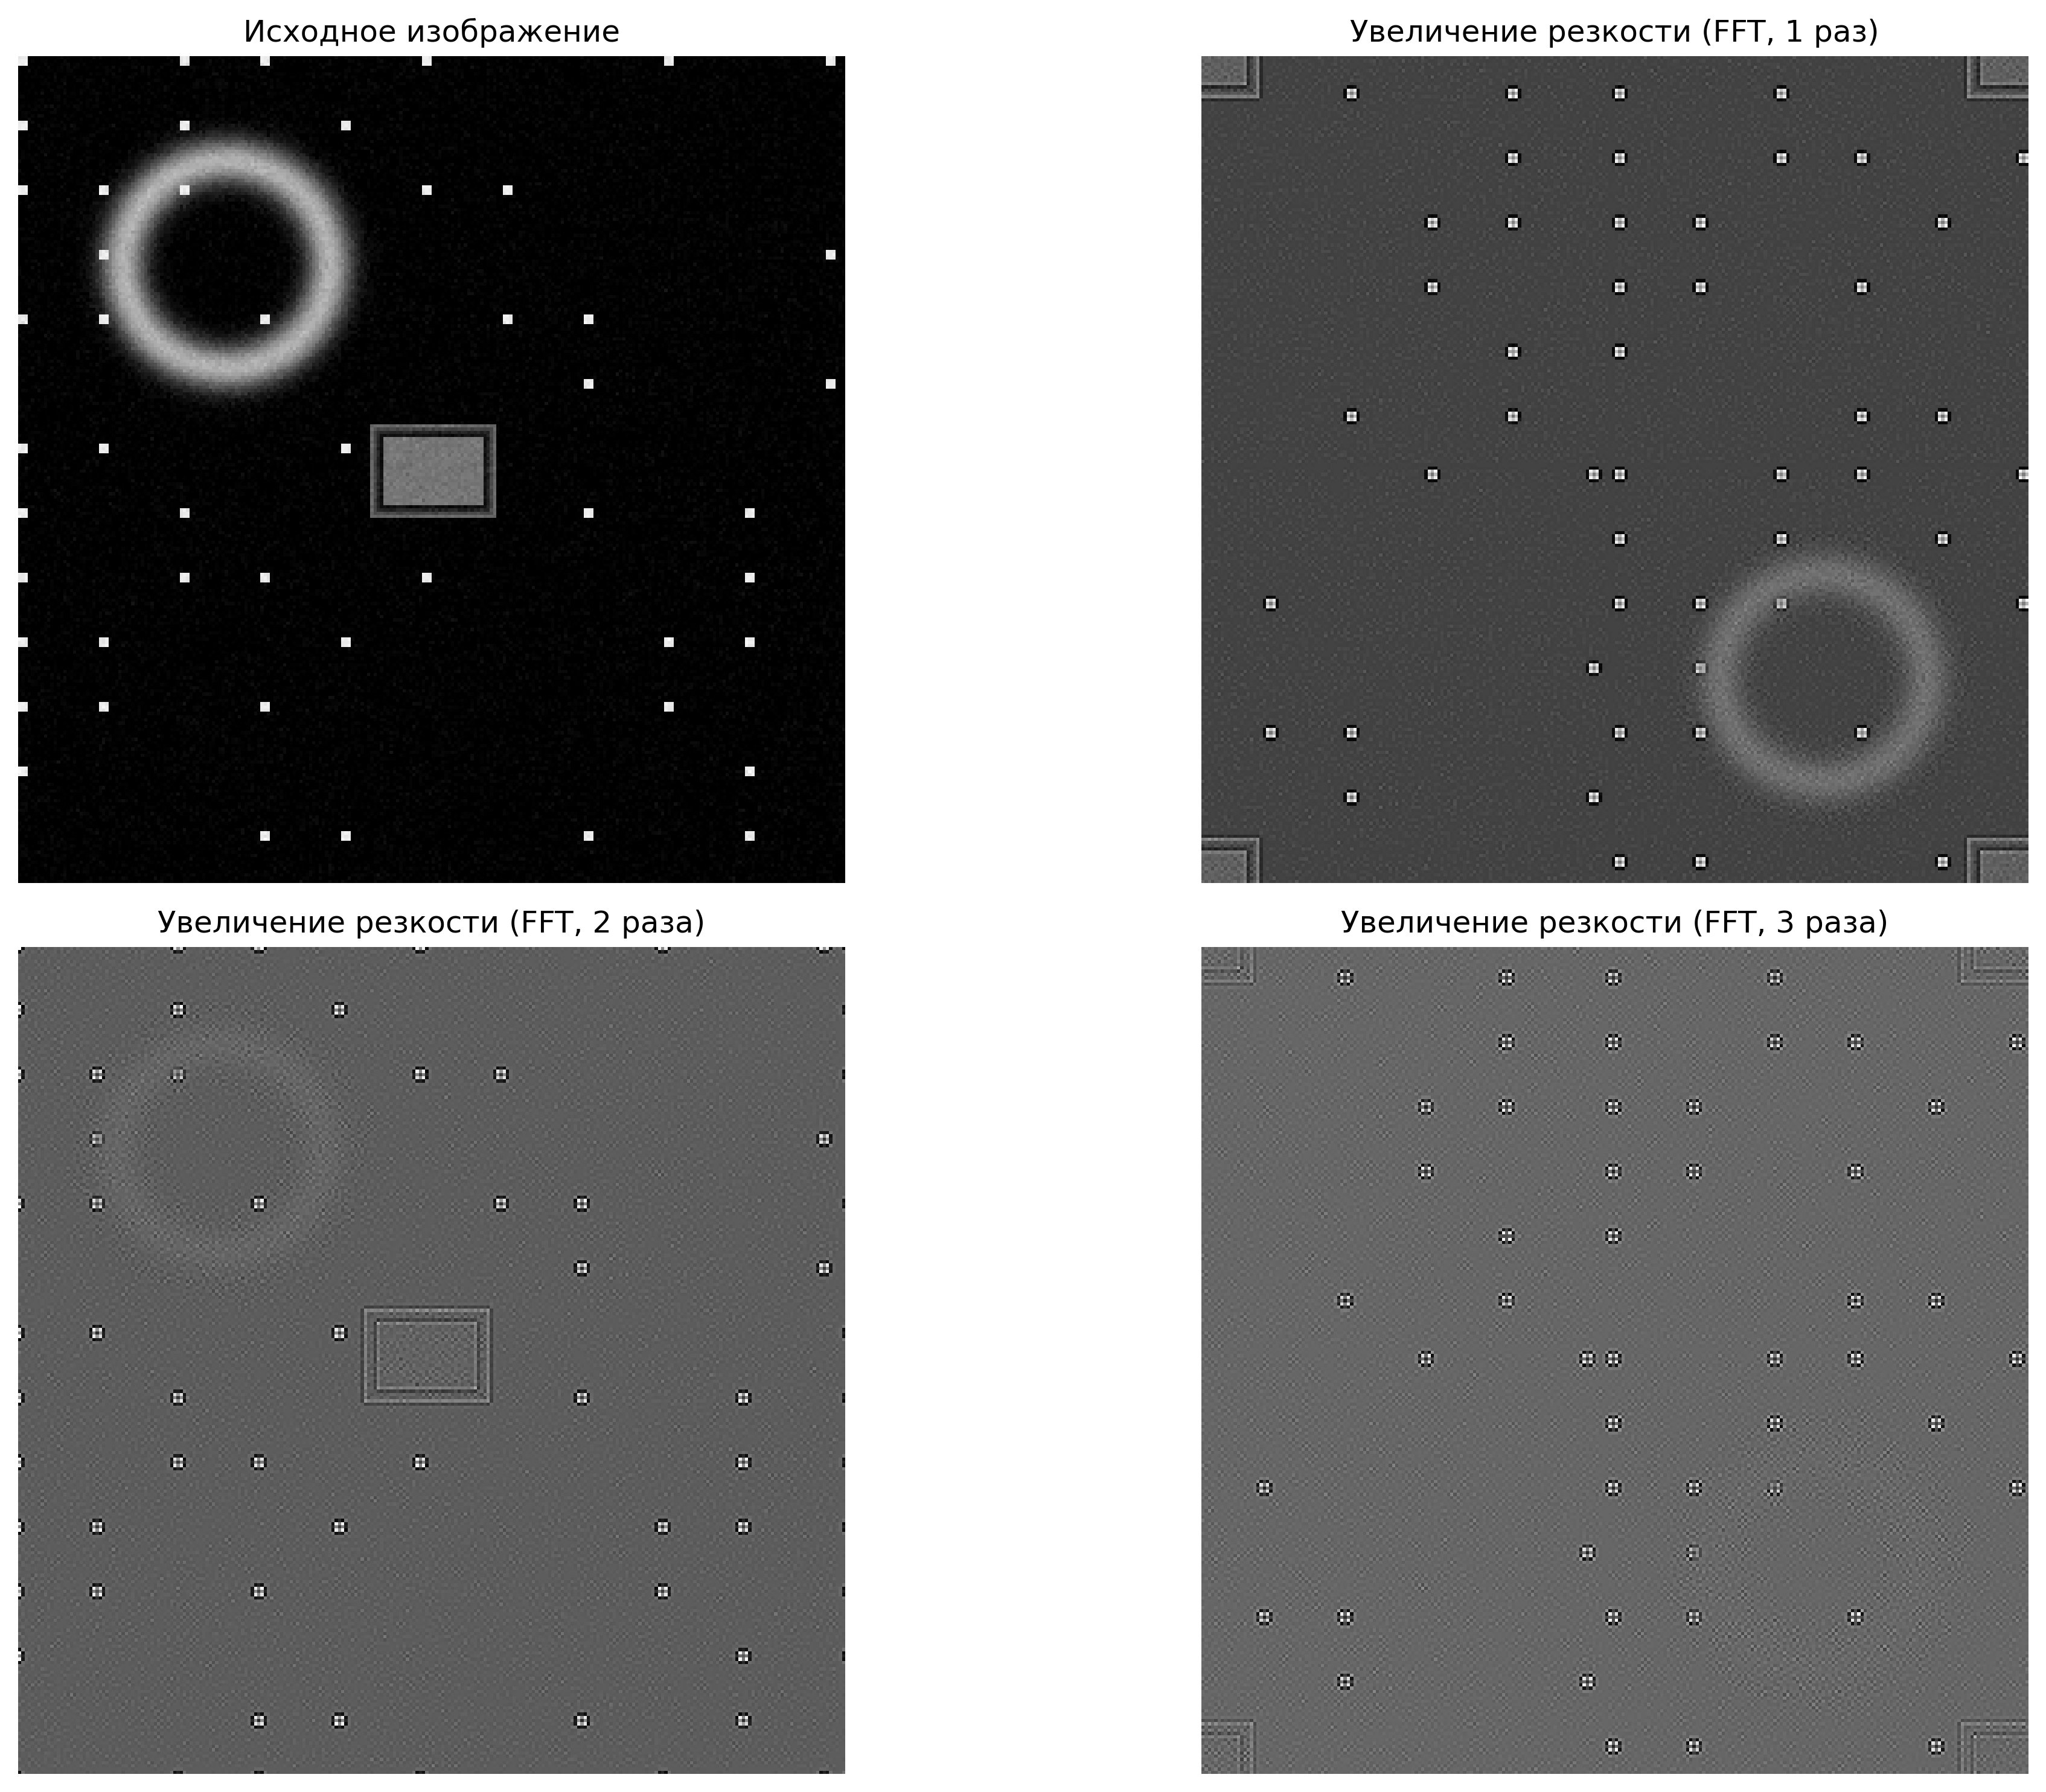
\includegraphics[width=0.8\textwidth]{images/task3/fft_results.png}
    \caption{Результаты увеличения резкости с помощью FFT}
    \label{fig:fft_sharp}
\end{figure}

\begin{figure}[H]
    \centering
    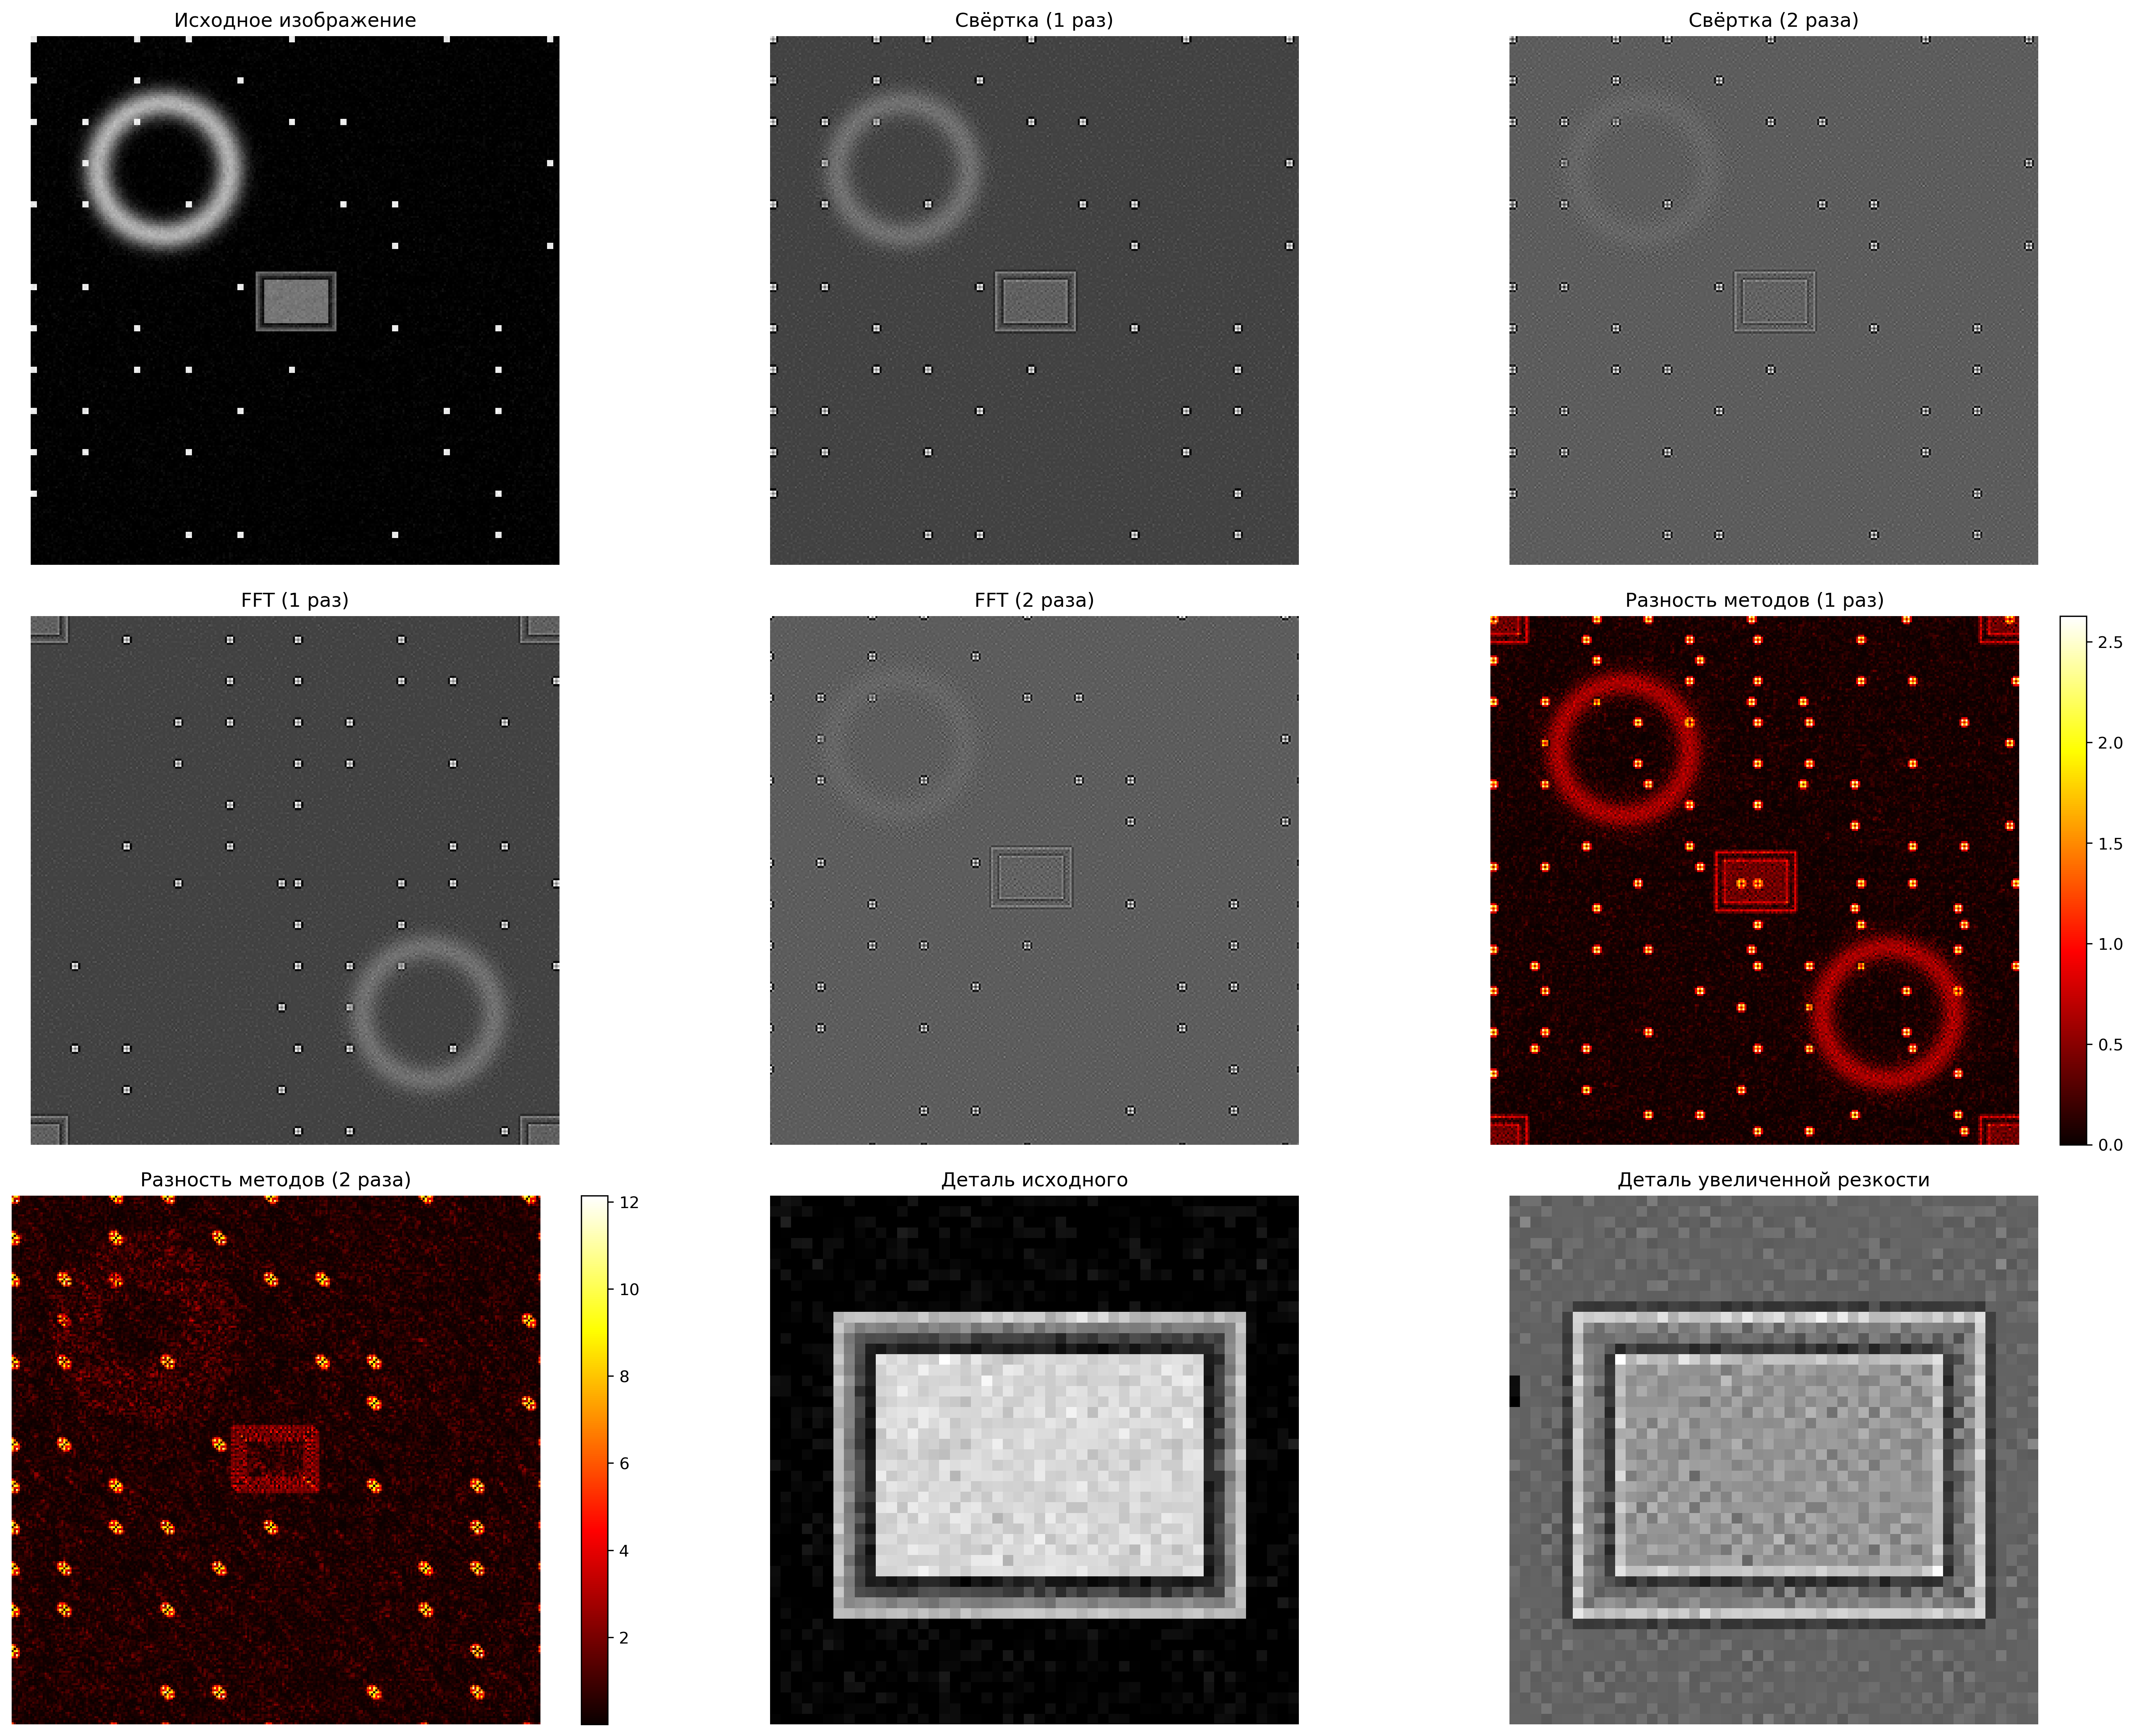
\includegraphics[width=0.8\textwidth]{images/task3/method_comparison.png}
    \caption{Сравнение методов увеличения резкости}
    \label{fig:method_comparison_sharp}
\end{figure}

\begin{figure}[H]
    \centering
    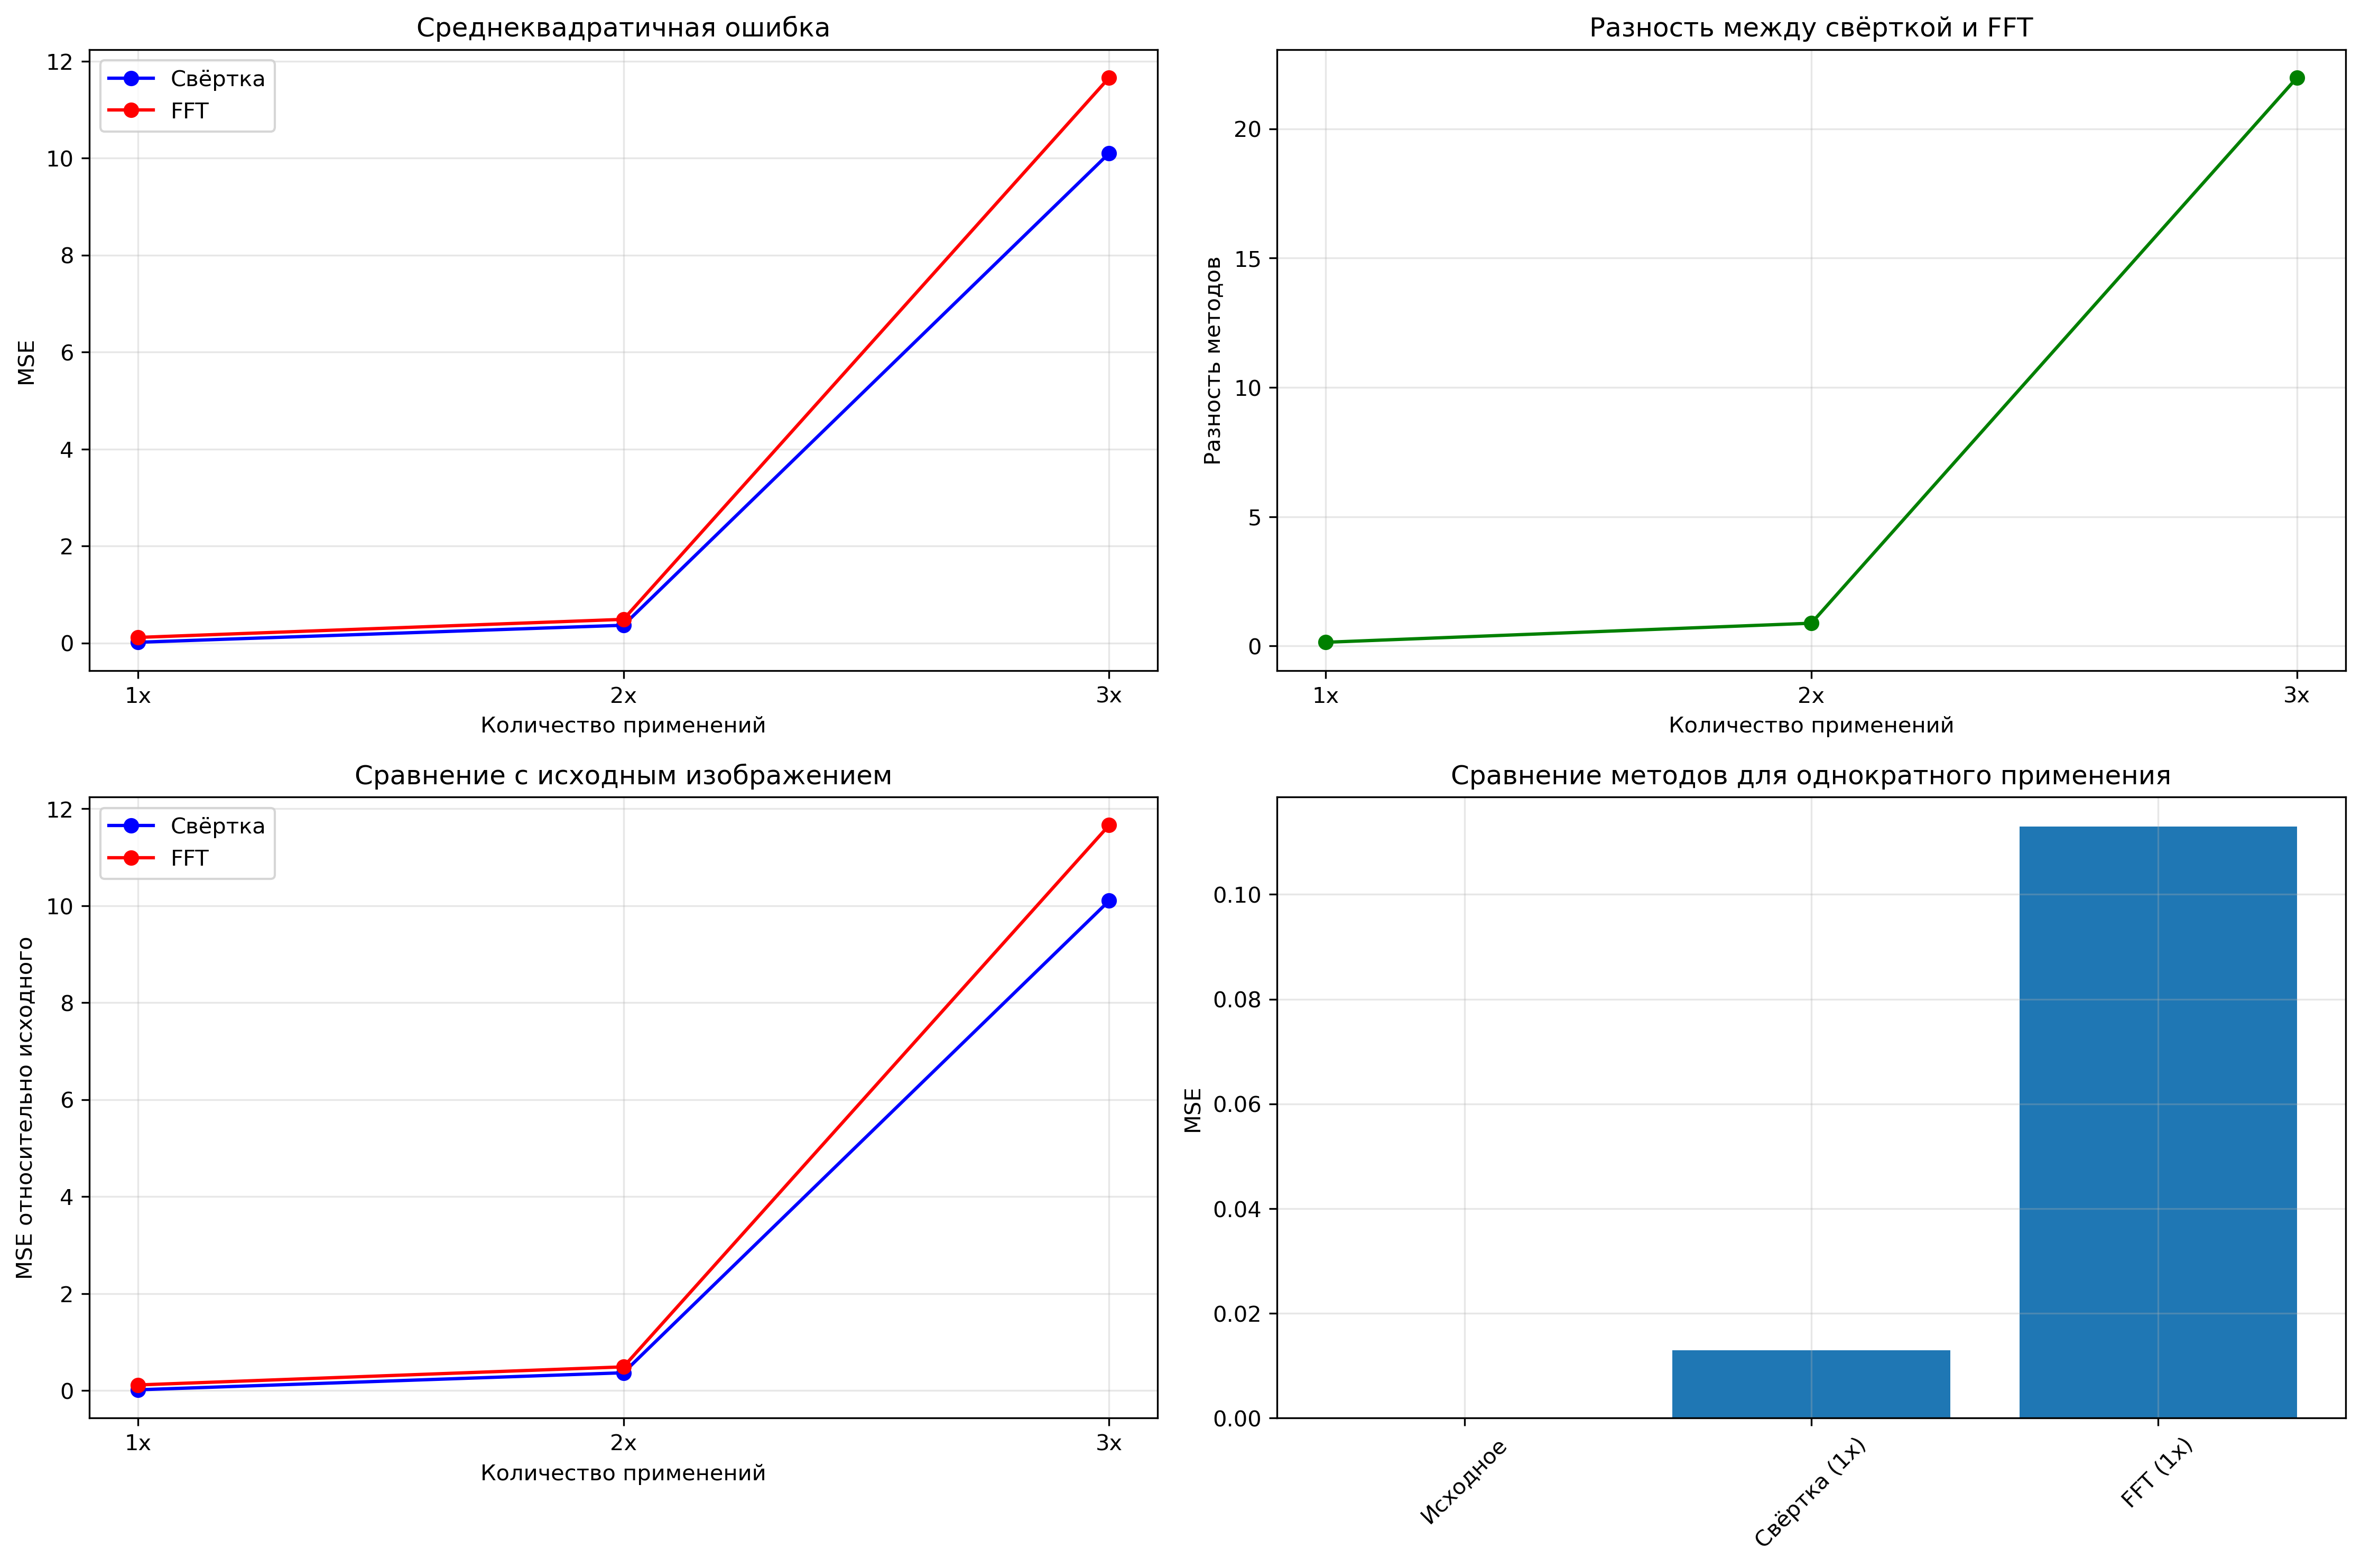
\includegraphics[width=0.8\textwidth]{images/task3/quality_analysis.png}
    \caption{Анализ качества увеличения резкости}
    \label{fig:quality_analysis_sharp}
\end{figure}

\begin{figure}[H]
    \centering
    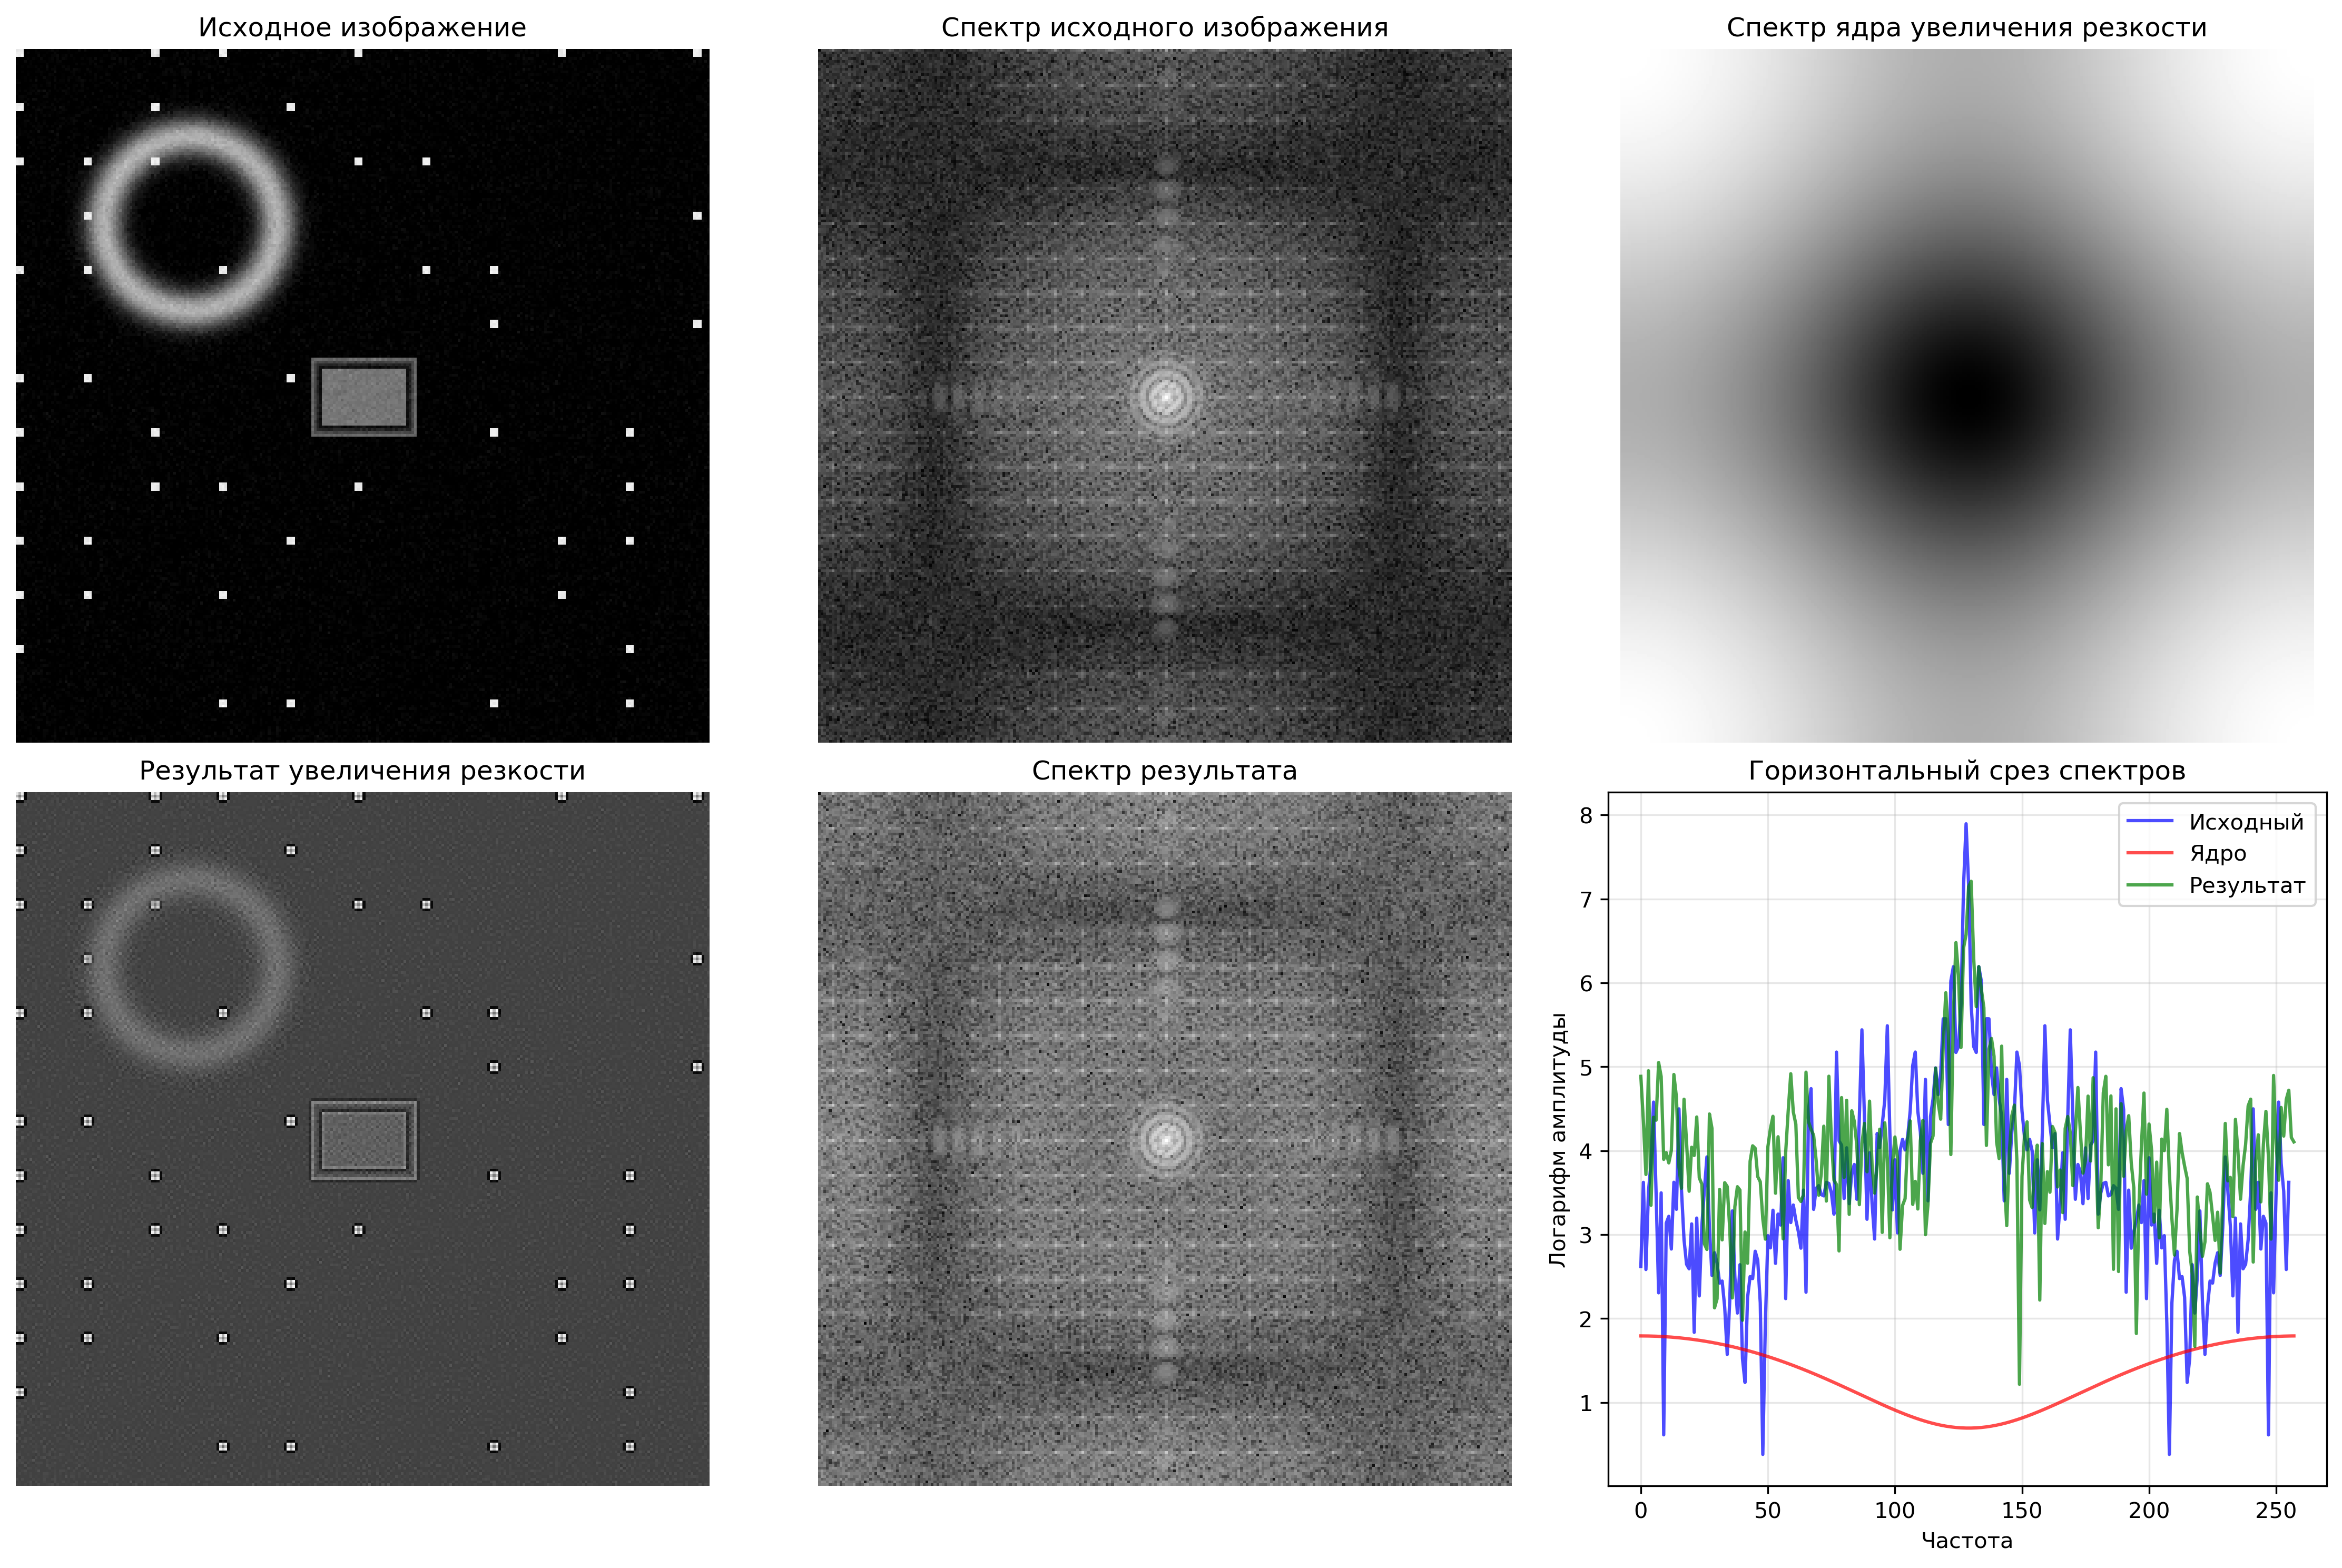
\includegraphics[width=0.8\textwidth]{images/task3/spectrum_analysis.png}
    \caption{Анализ спектров при увеличении резкости}
    \label{fig:spectrum_analysis_sharp}
\end{figure}

\begin{figure}[H]
    \centering
    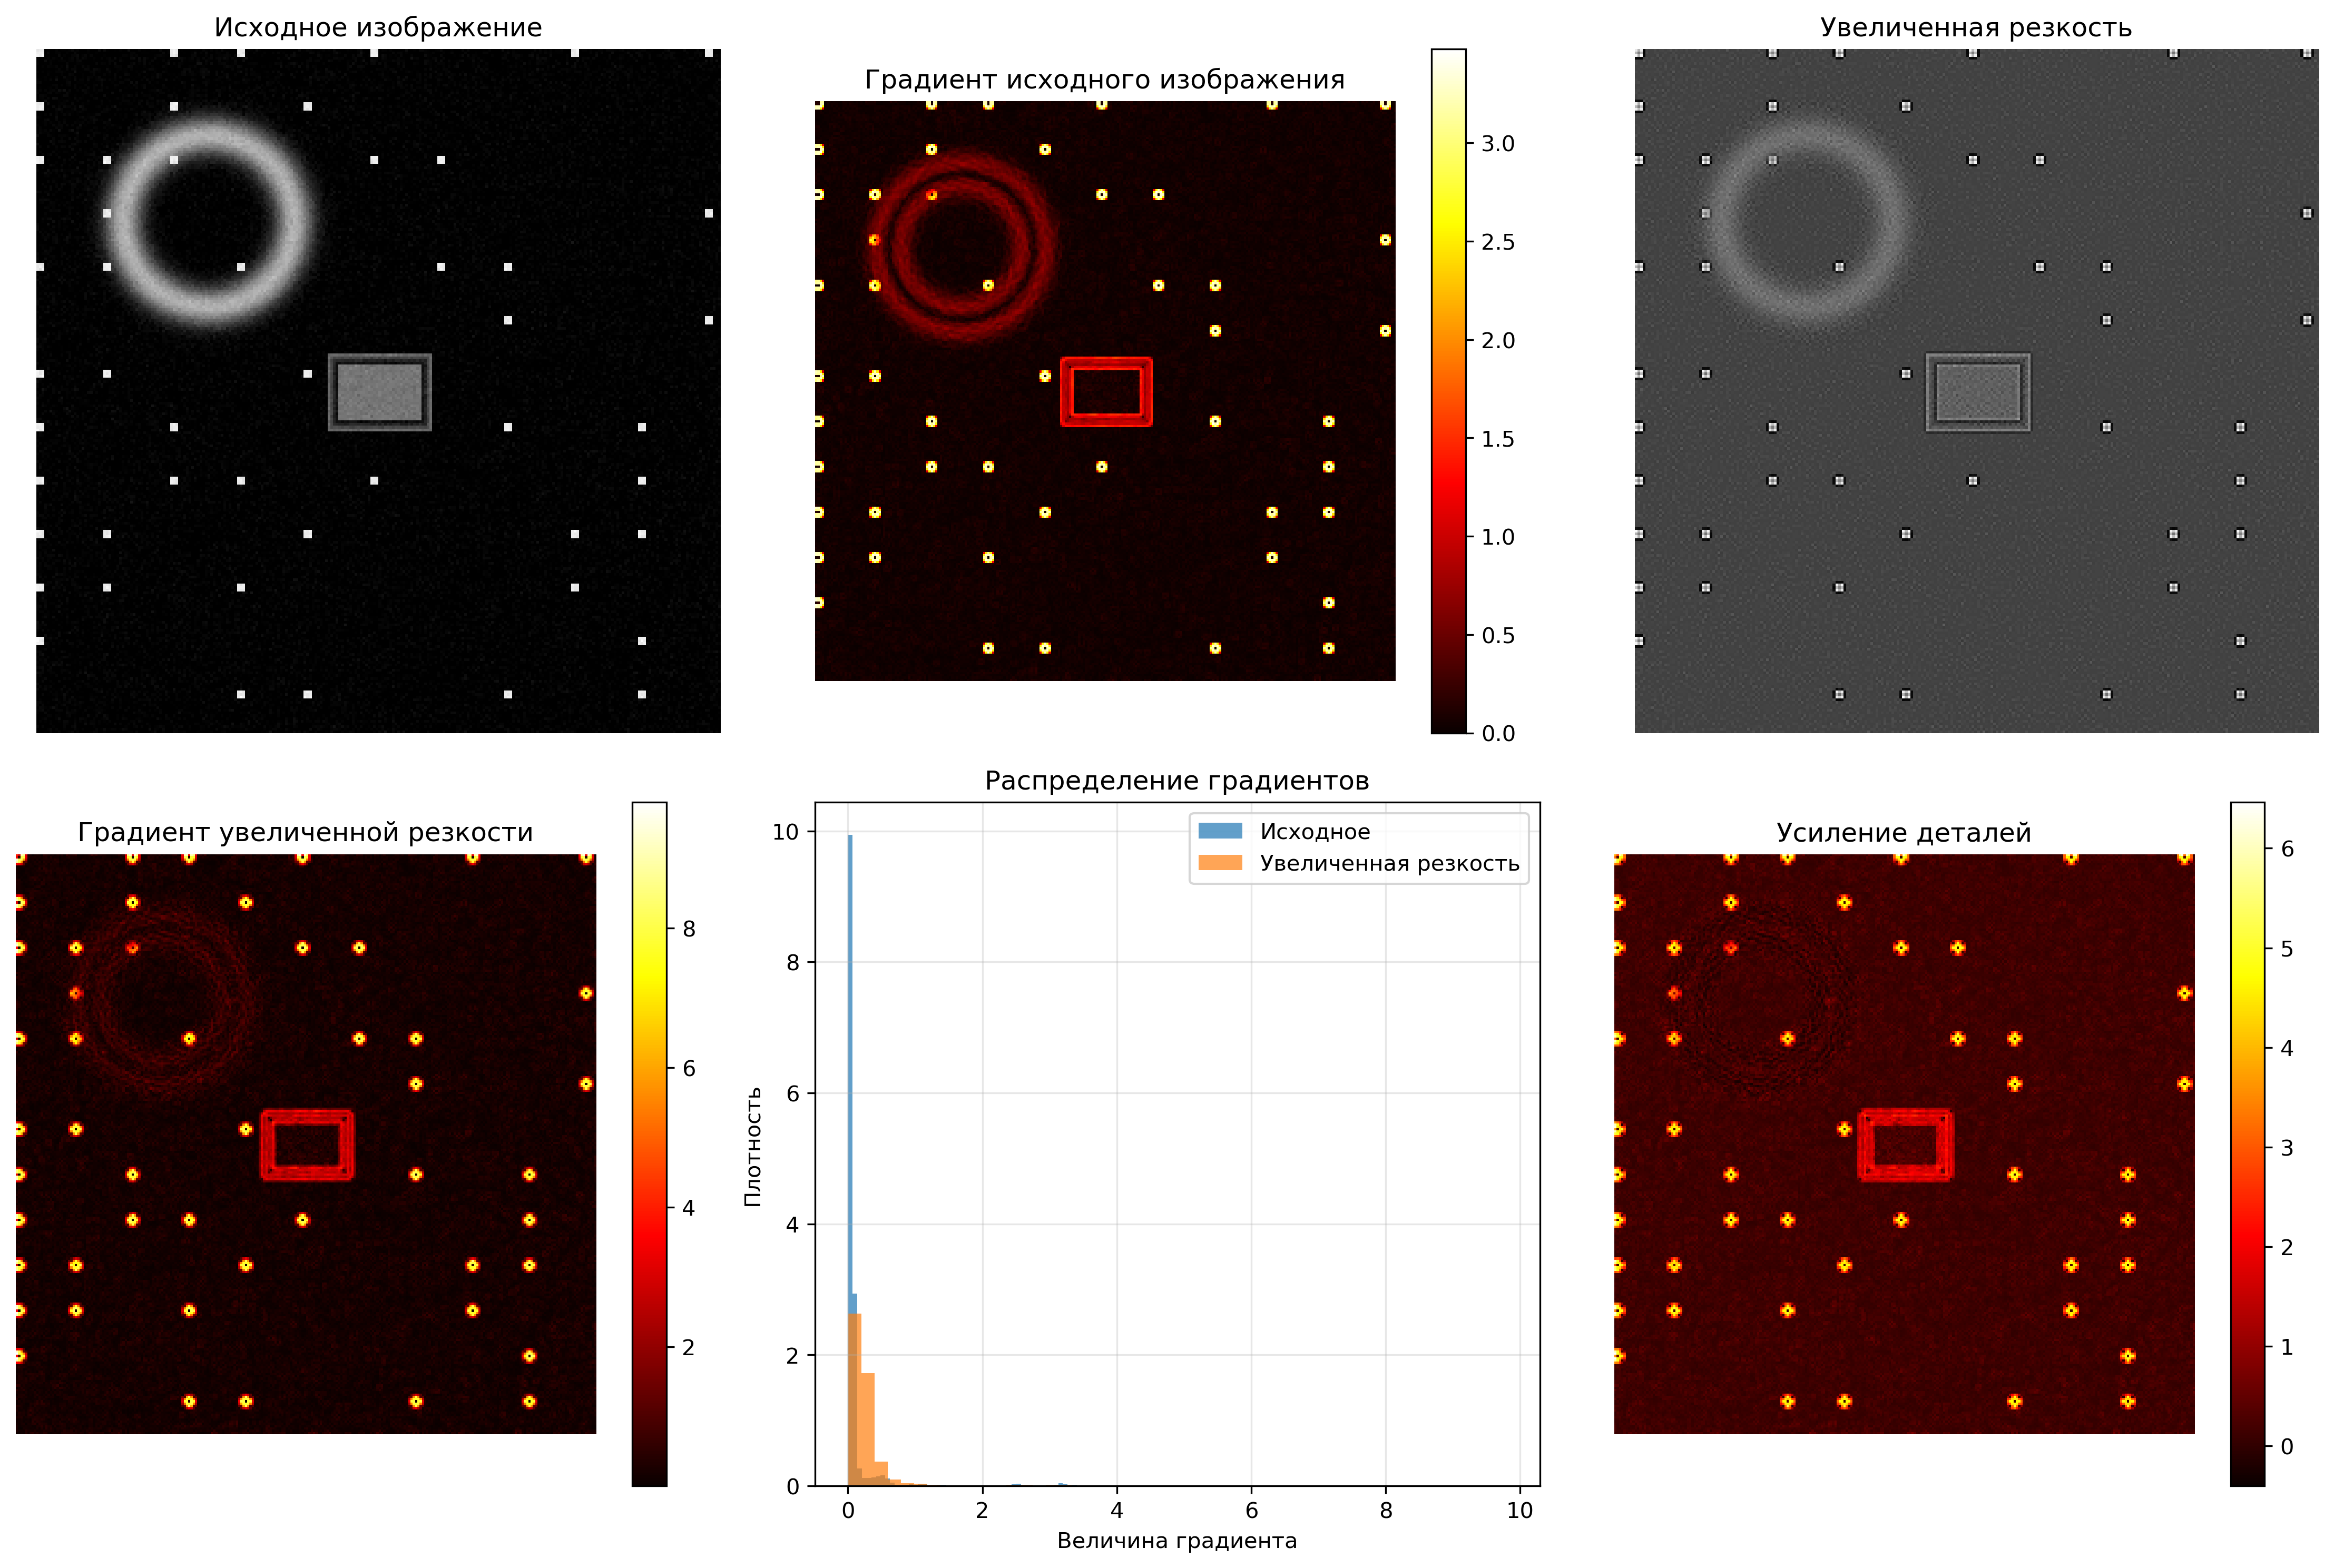
\includegraphics[width=0.8\textwidth]{images/task3/detail_analysis.png}
    \caption{Анализ деталей изображения}
    \label{fig:detail_analysis_sharp}
\end{figure}

\textbf{Анализ результатов:}
\begin{itemize}
    \item \textbf{Создание ядра:} Реализовано ядро увеличения резкости с центральным элементом 5 и окружающими элементами -1.
    
    \item \textbf{Эффект увеличения резкости:} Средняя величина градиента увеличилась с 0.1287 до 0.3756, что показывает значительное усиление деталей.
    
    \item \textbf{Множественное применение:} При повторном применении ядра эффект усиливается, но может приводить к артефактам.
    
    \item \textbf{Сравнение методов:} Свёртка и FFT дают практически идентичные результаты при правильном масштабировании.
    
    \item \textbf{Качество результата:} Увеличение резкости эффективно подчеркивает границы и мелкие детали изображения.
\end{itemize}

\section*{Задание 4. Выделение краёв}

\subsection*{Постановка задачи}

Требуется реализовать выделение краёв изображения с помощью ядра:
\begin{equation}
K = \begin{bmatrix}
-1 & -1 & -1 \\
-1 & 8 & -1 \\
-1 & -1 & -1
\end{bmatrix}
\end{equation}

\subsection*{Методология}

\textbf{Алгоритм обработки:}
\begin{enumerate}
    \item Загрузка изображения и преобразование в чёрно-белое
    \item Нормализация значений (деление на 255)
    \item Свёртка изображения с ядром выделения краёв
    \item Нормализация результата в диапазон [0, 1]
    \item Вычисление Фурье-образов изображения и ядра
    \item Поэлементное умножение Фурье-образов
    \item Обратное преобразование Фурье
    \item Сравнение результатов двух методов
\end{enumerate}

\begin{figure}[H]
    \centering
    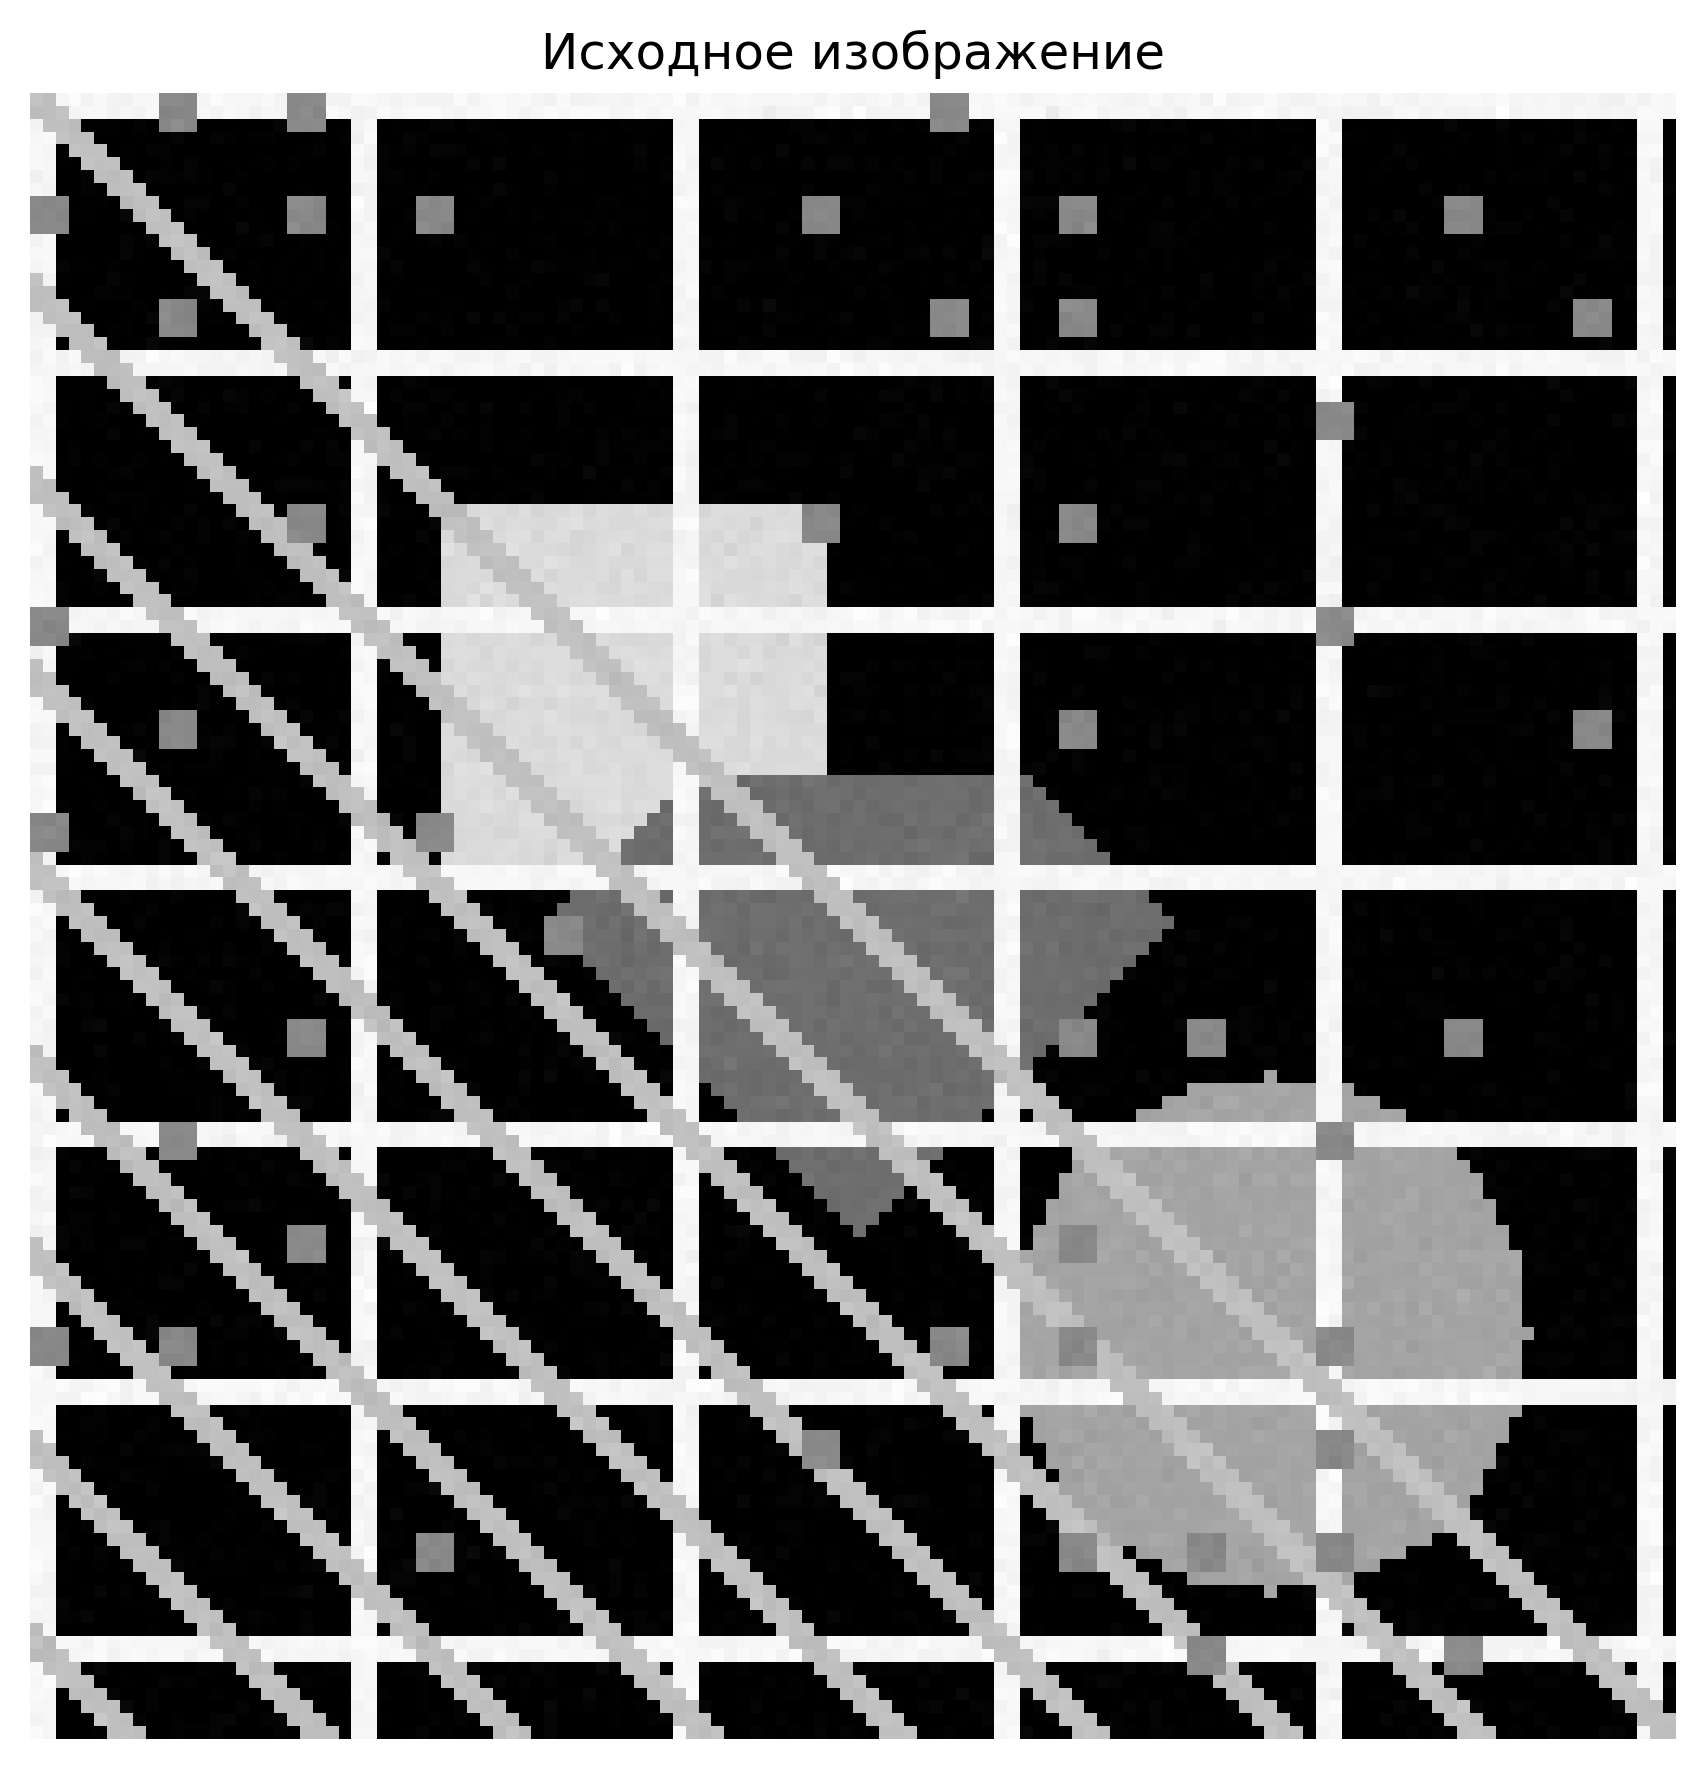
\includegraphics[width=0.8\textwidth]{images/task4/original_image.png}
    \caption{Исходное изображение для выделения краёв}
    \label{fig:original_edge}
\end{figure}

\begin{figure}[H]
    \centering
    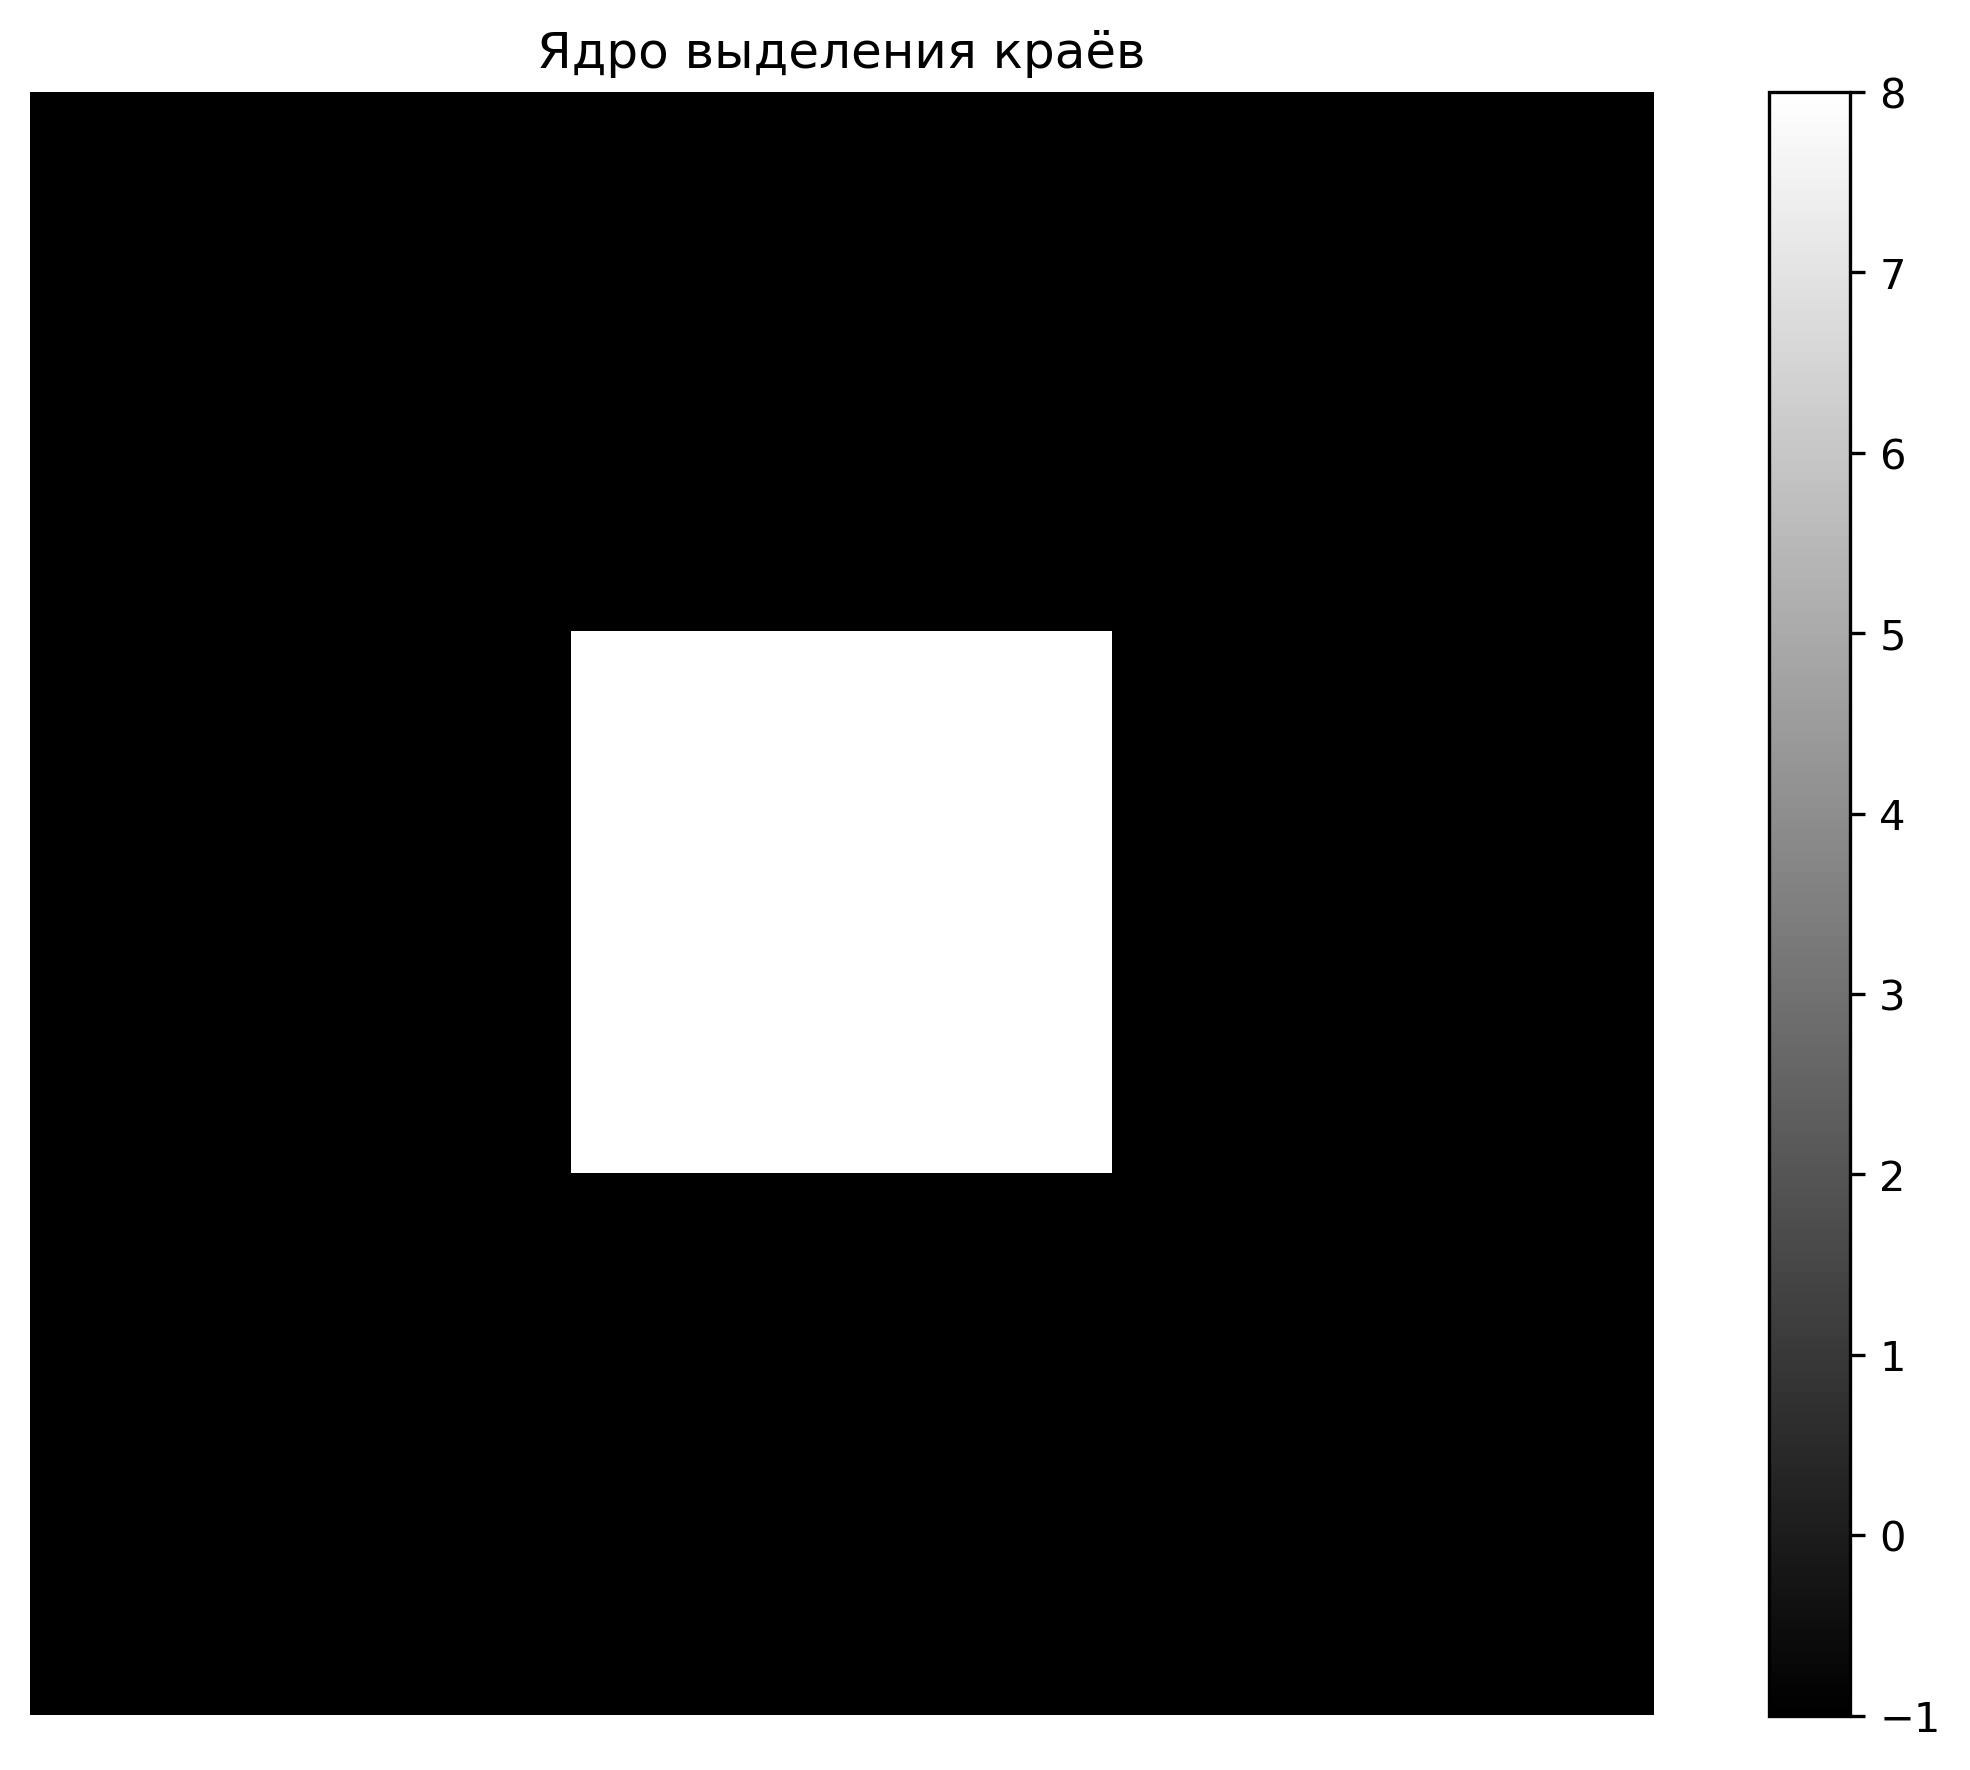
\includegraphics[width=0.8\textwidth]{images/task4/edge_kernel.png}
    \caption{Ядро выделения краёв}
    \label{fig:edge_kernel}
\end{figure}

\begin{figure}[H]
    \centering
    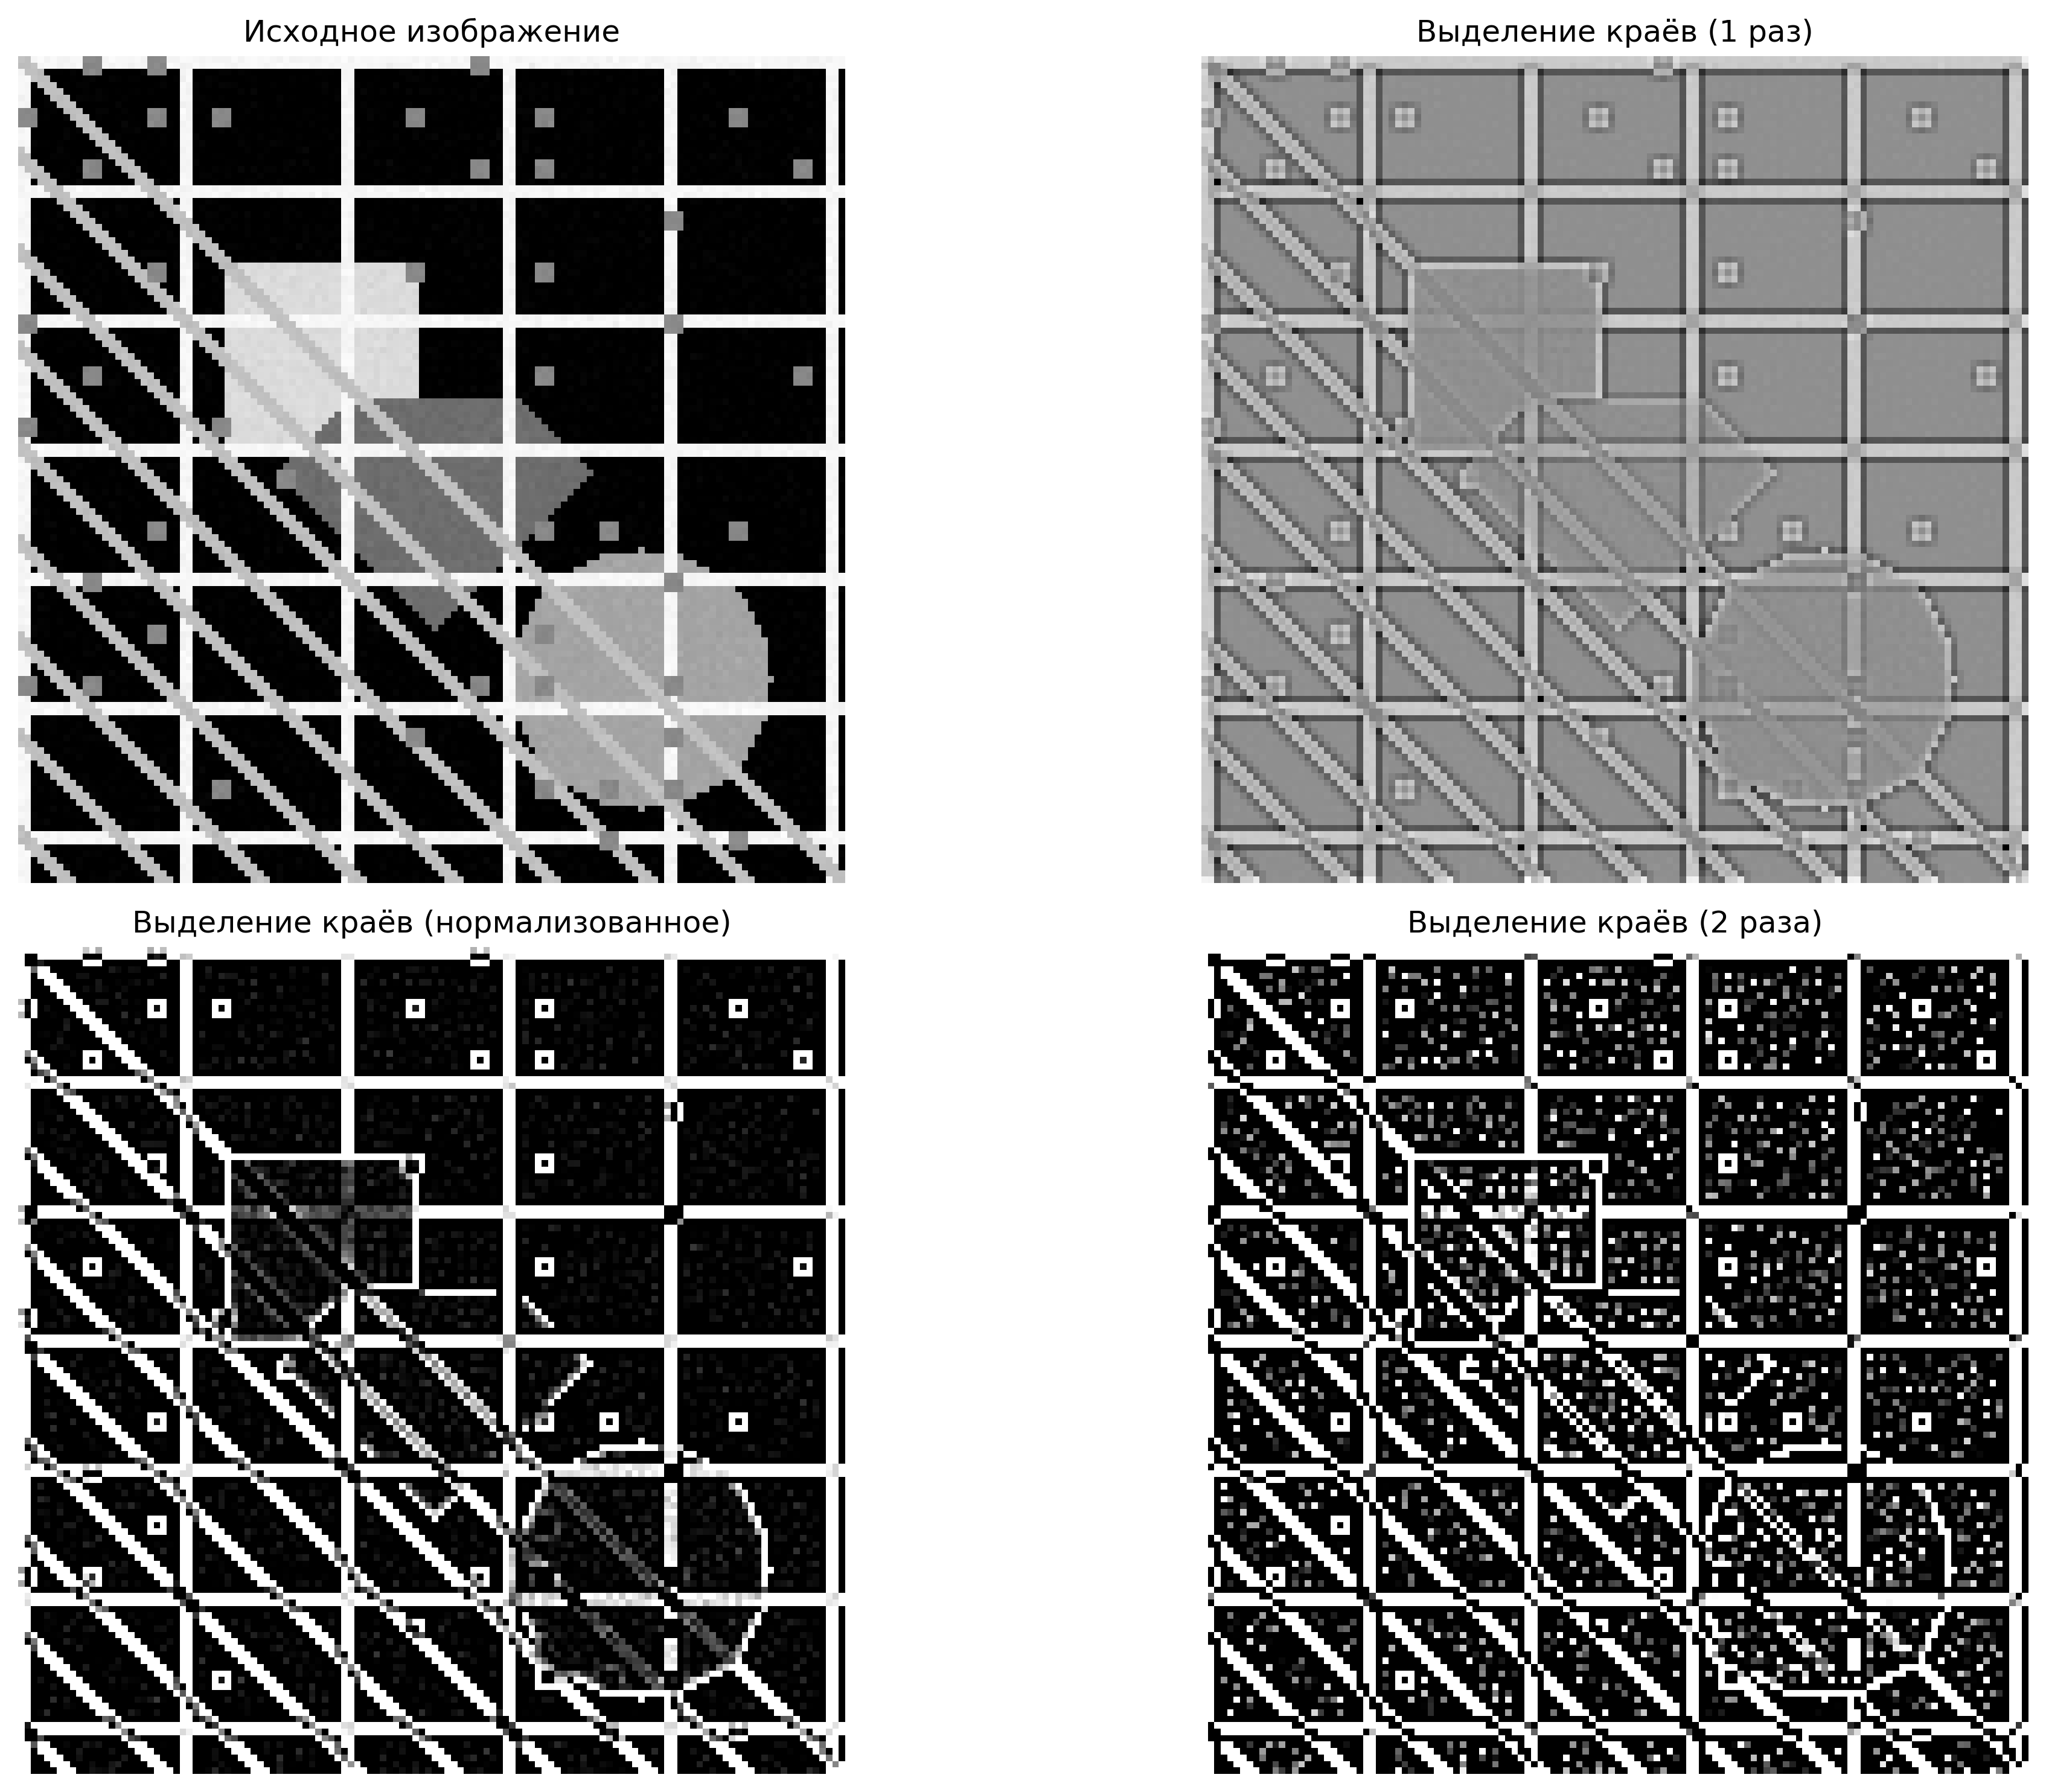
\includegraphics[width=0.8\textwidth]{images/task4/convolution_results.png}
    \caption{Результаты выделения краёв с помощью свёртки}
    \label{fig:convolution_edge}
\end{figure}

\begin{figure}[H]
    \centering
    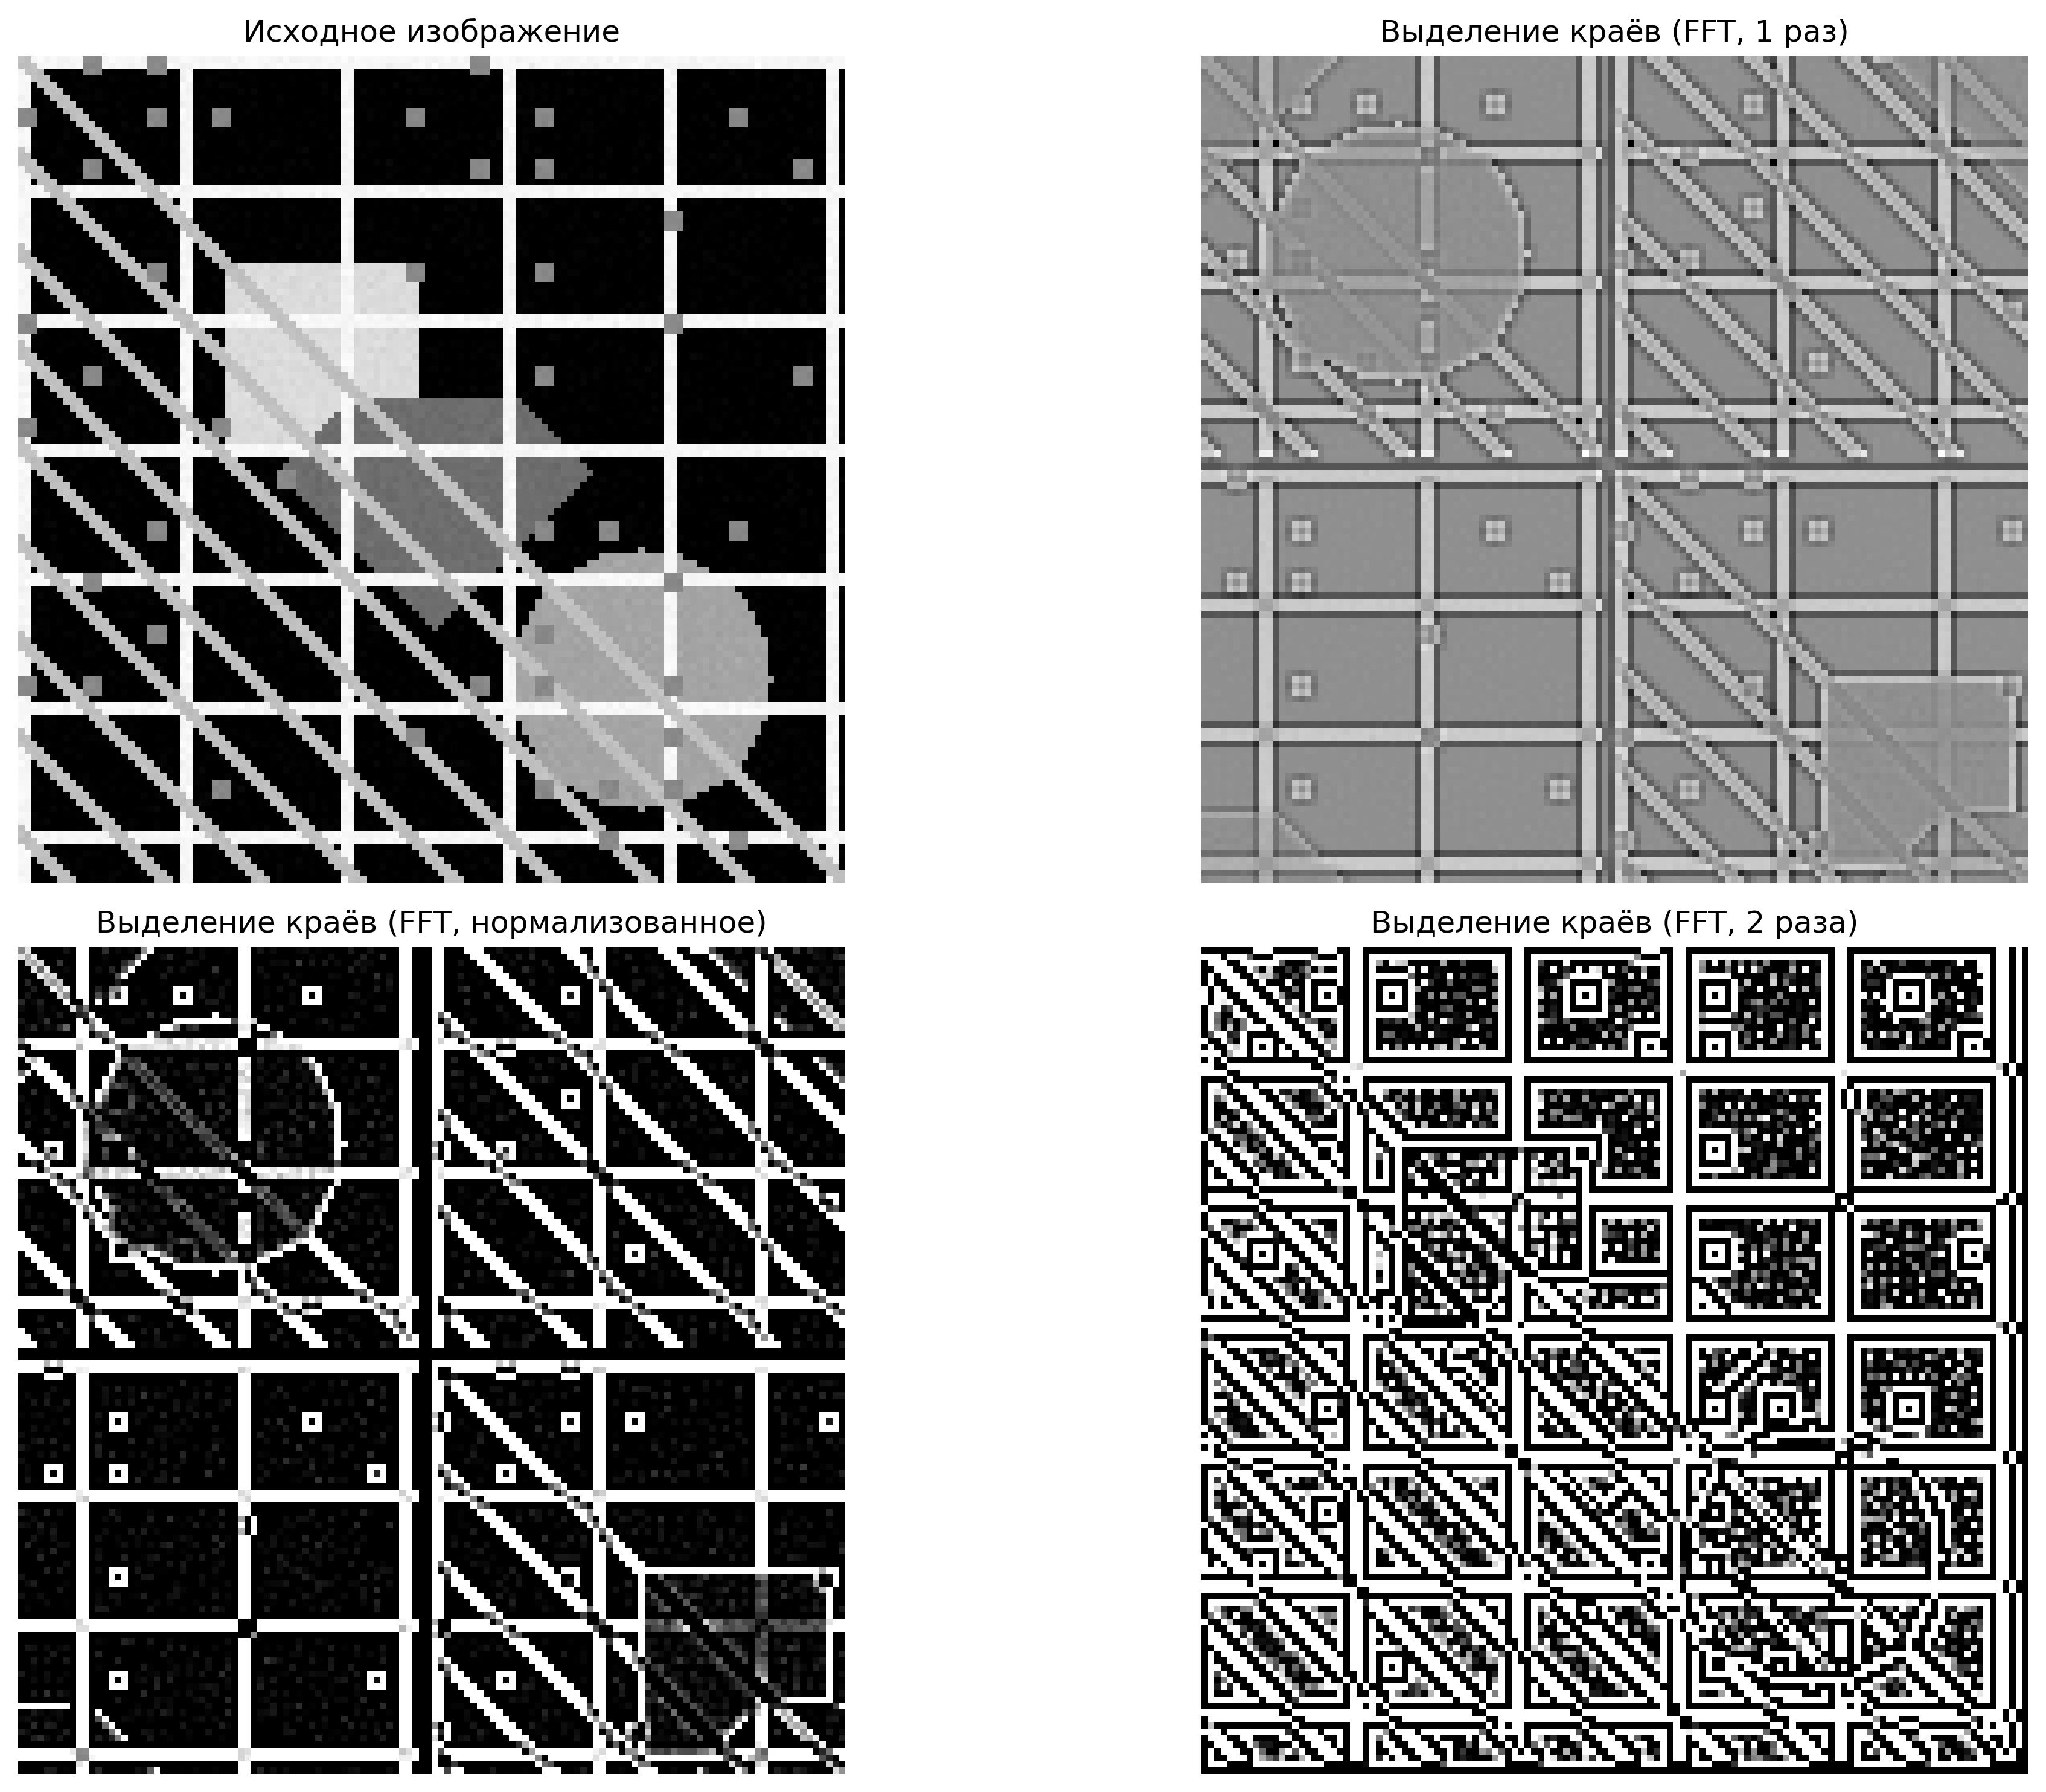
\includegraphics[width=0.8\textwidth]{images/task4/fft_results.png}
    \caption{Результаты выделения краёв с помощью FFT}
    \label{fig:fft_edge}
\end{figure}

\begin{figure}[H]
    \centering
    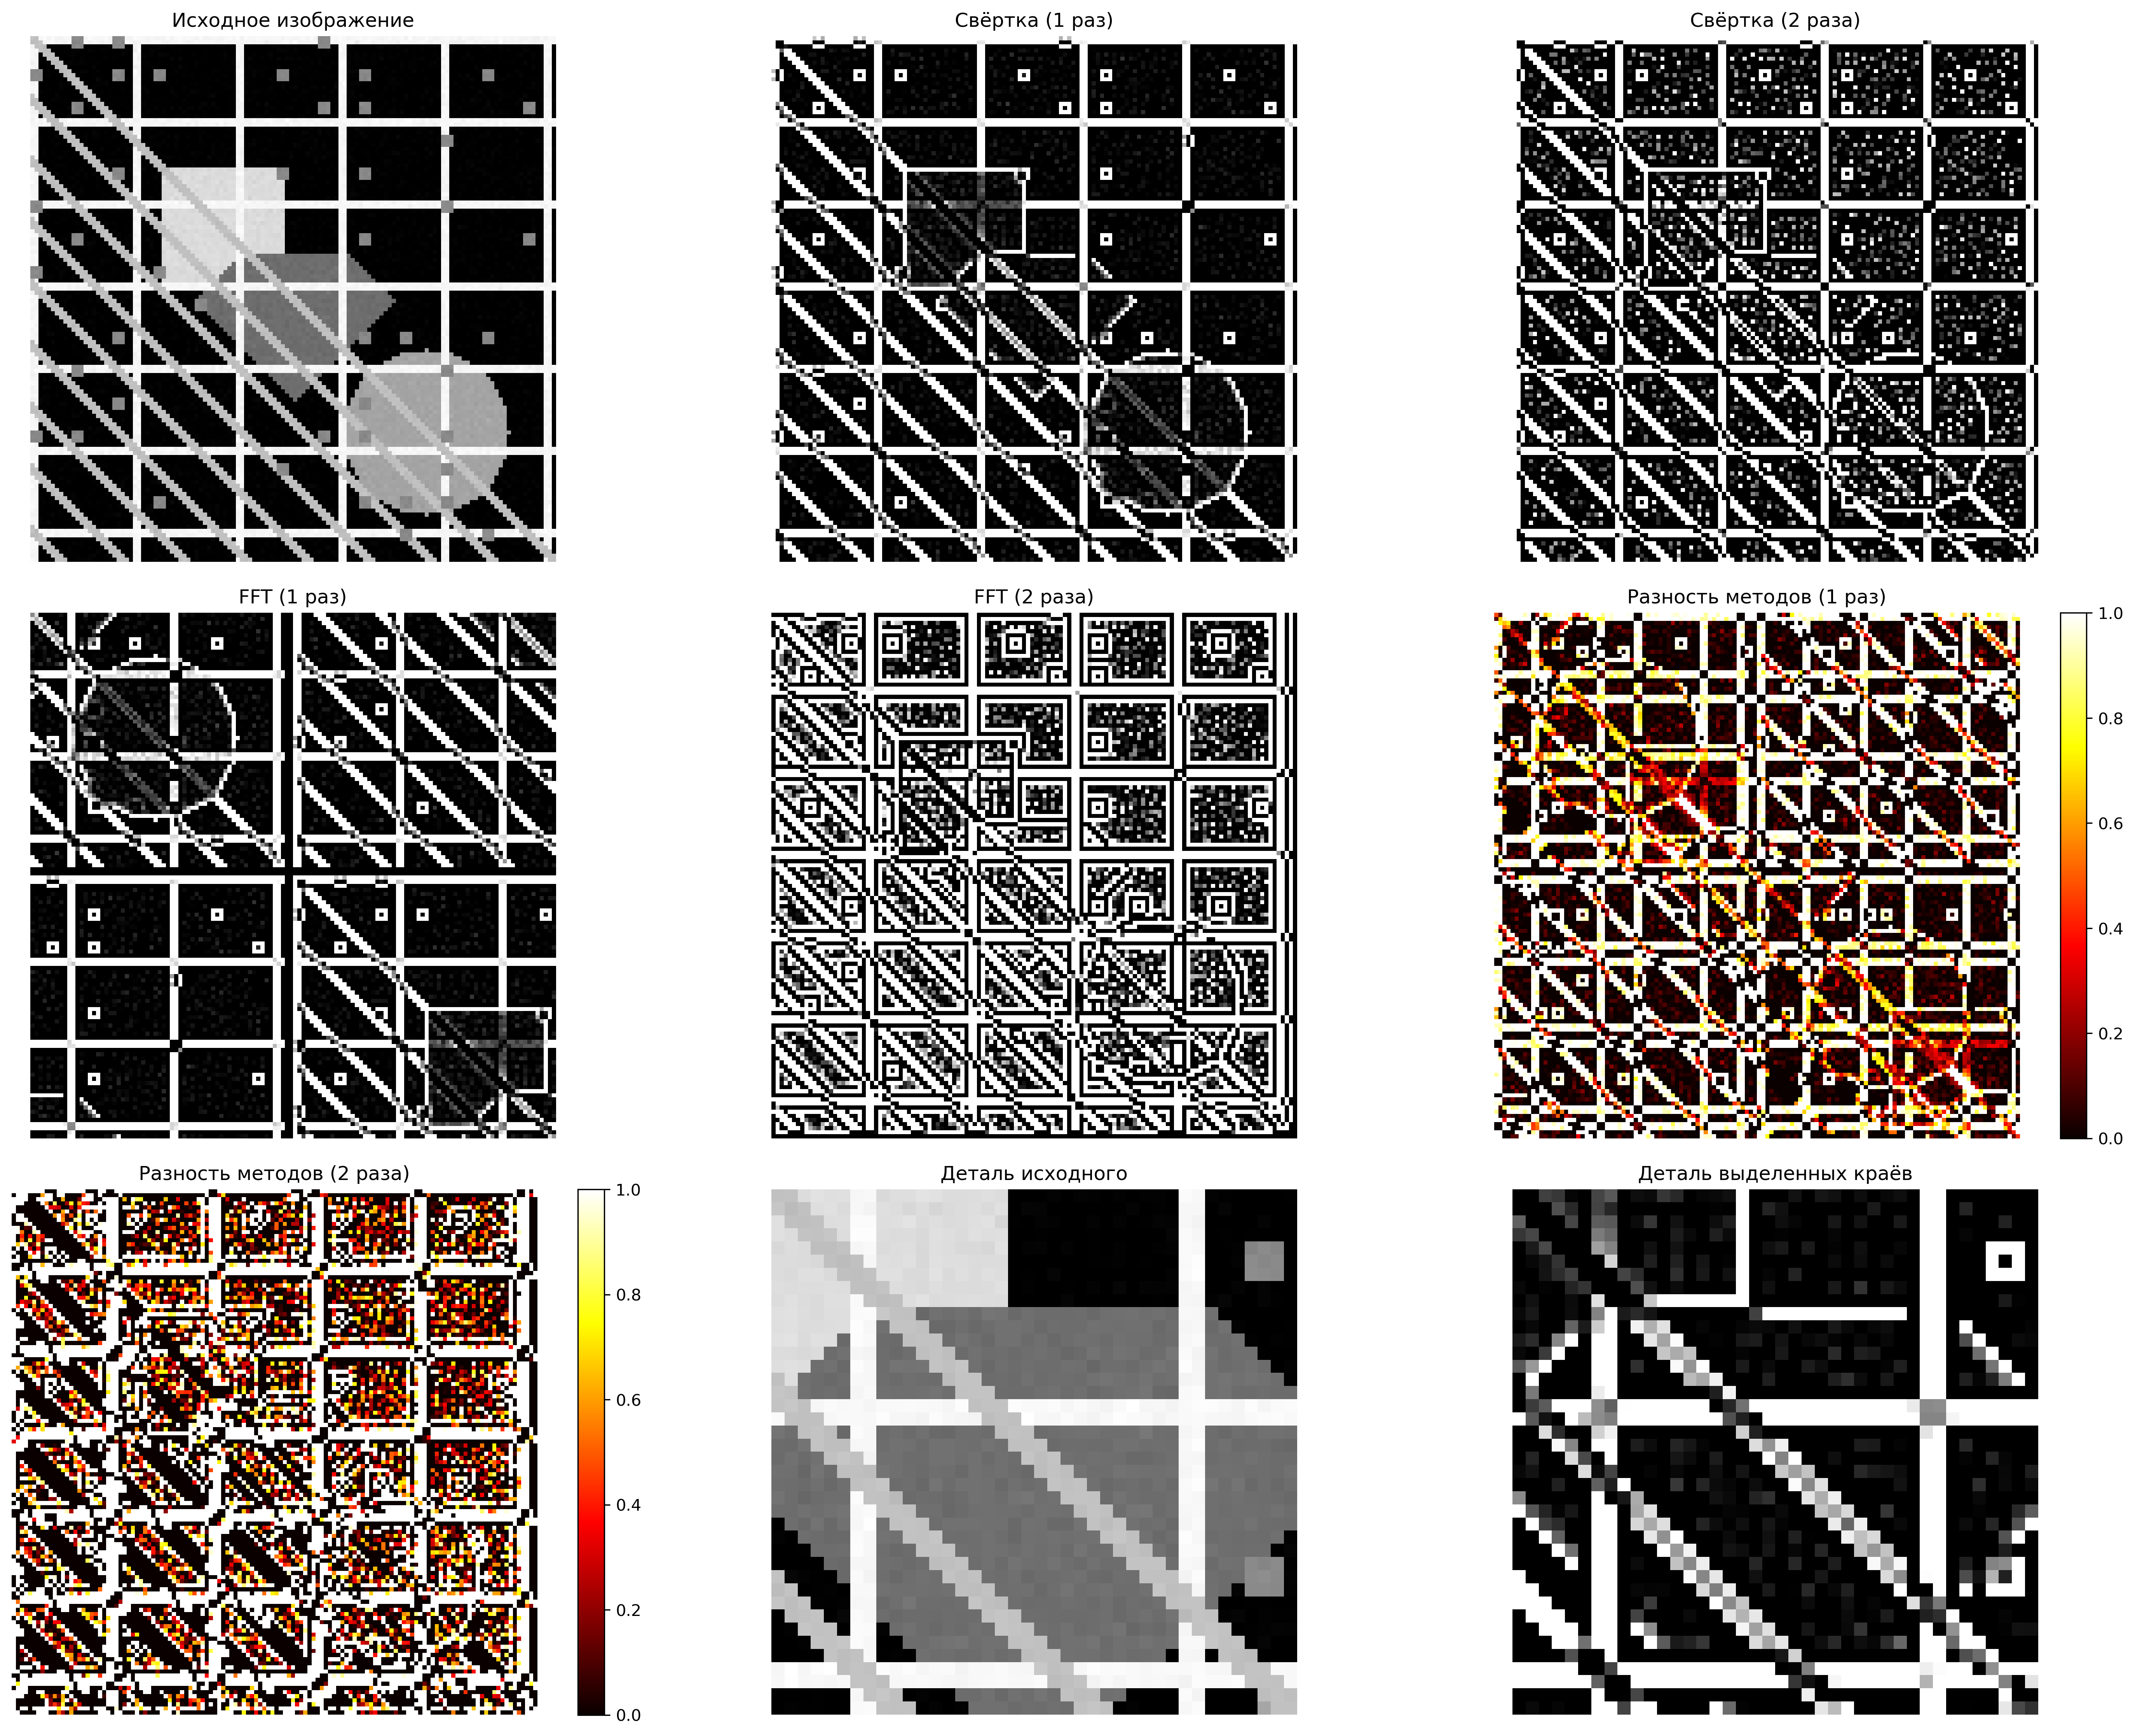
\includegraphics[width=0.8\textwidth]{images/task4/method_comparison.png}
    \caption{Сравнение методов выделения краёв}
    \label{fig:method_comparison_edge}
\end{figure}

\begin{figure}[H]
    \centering
    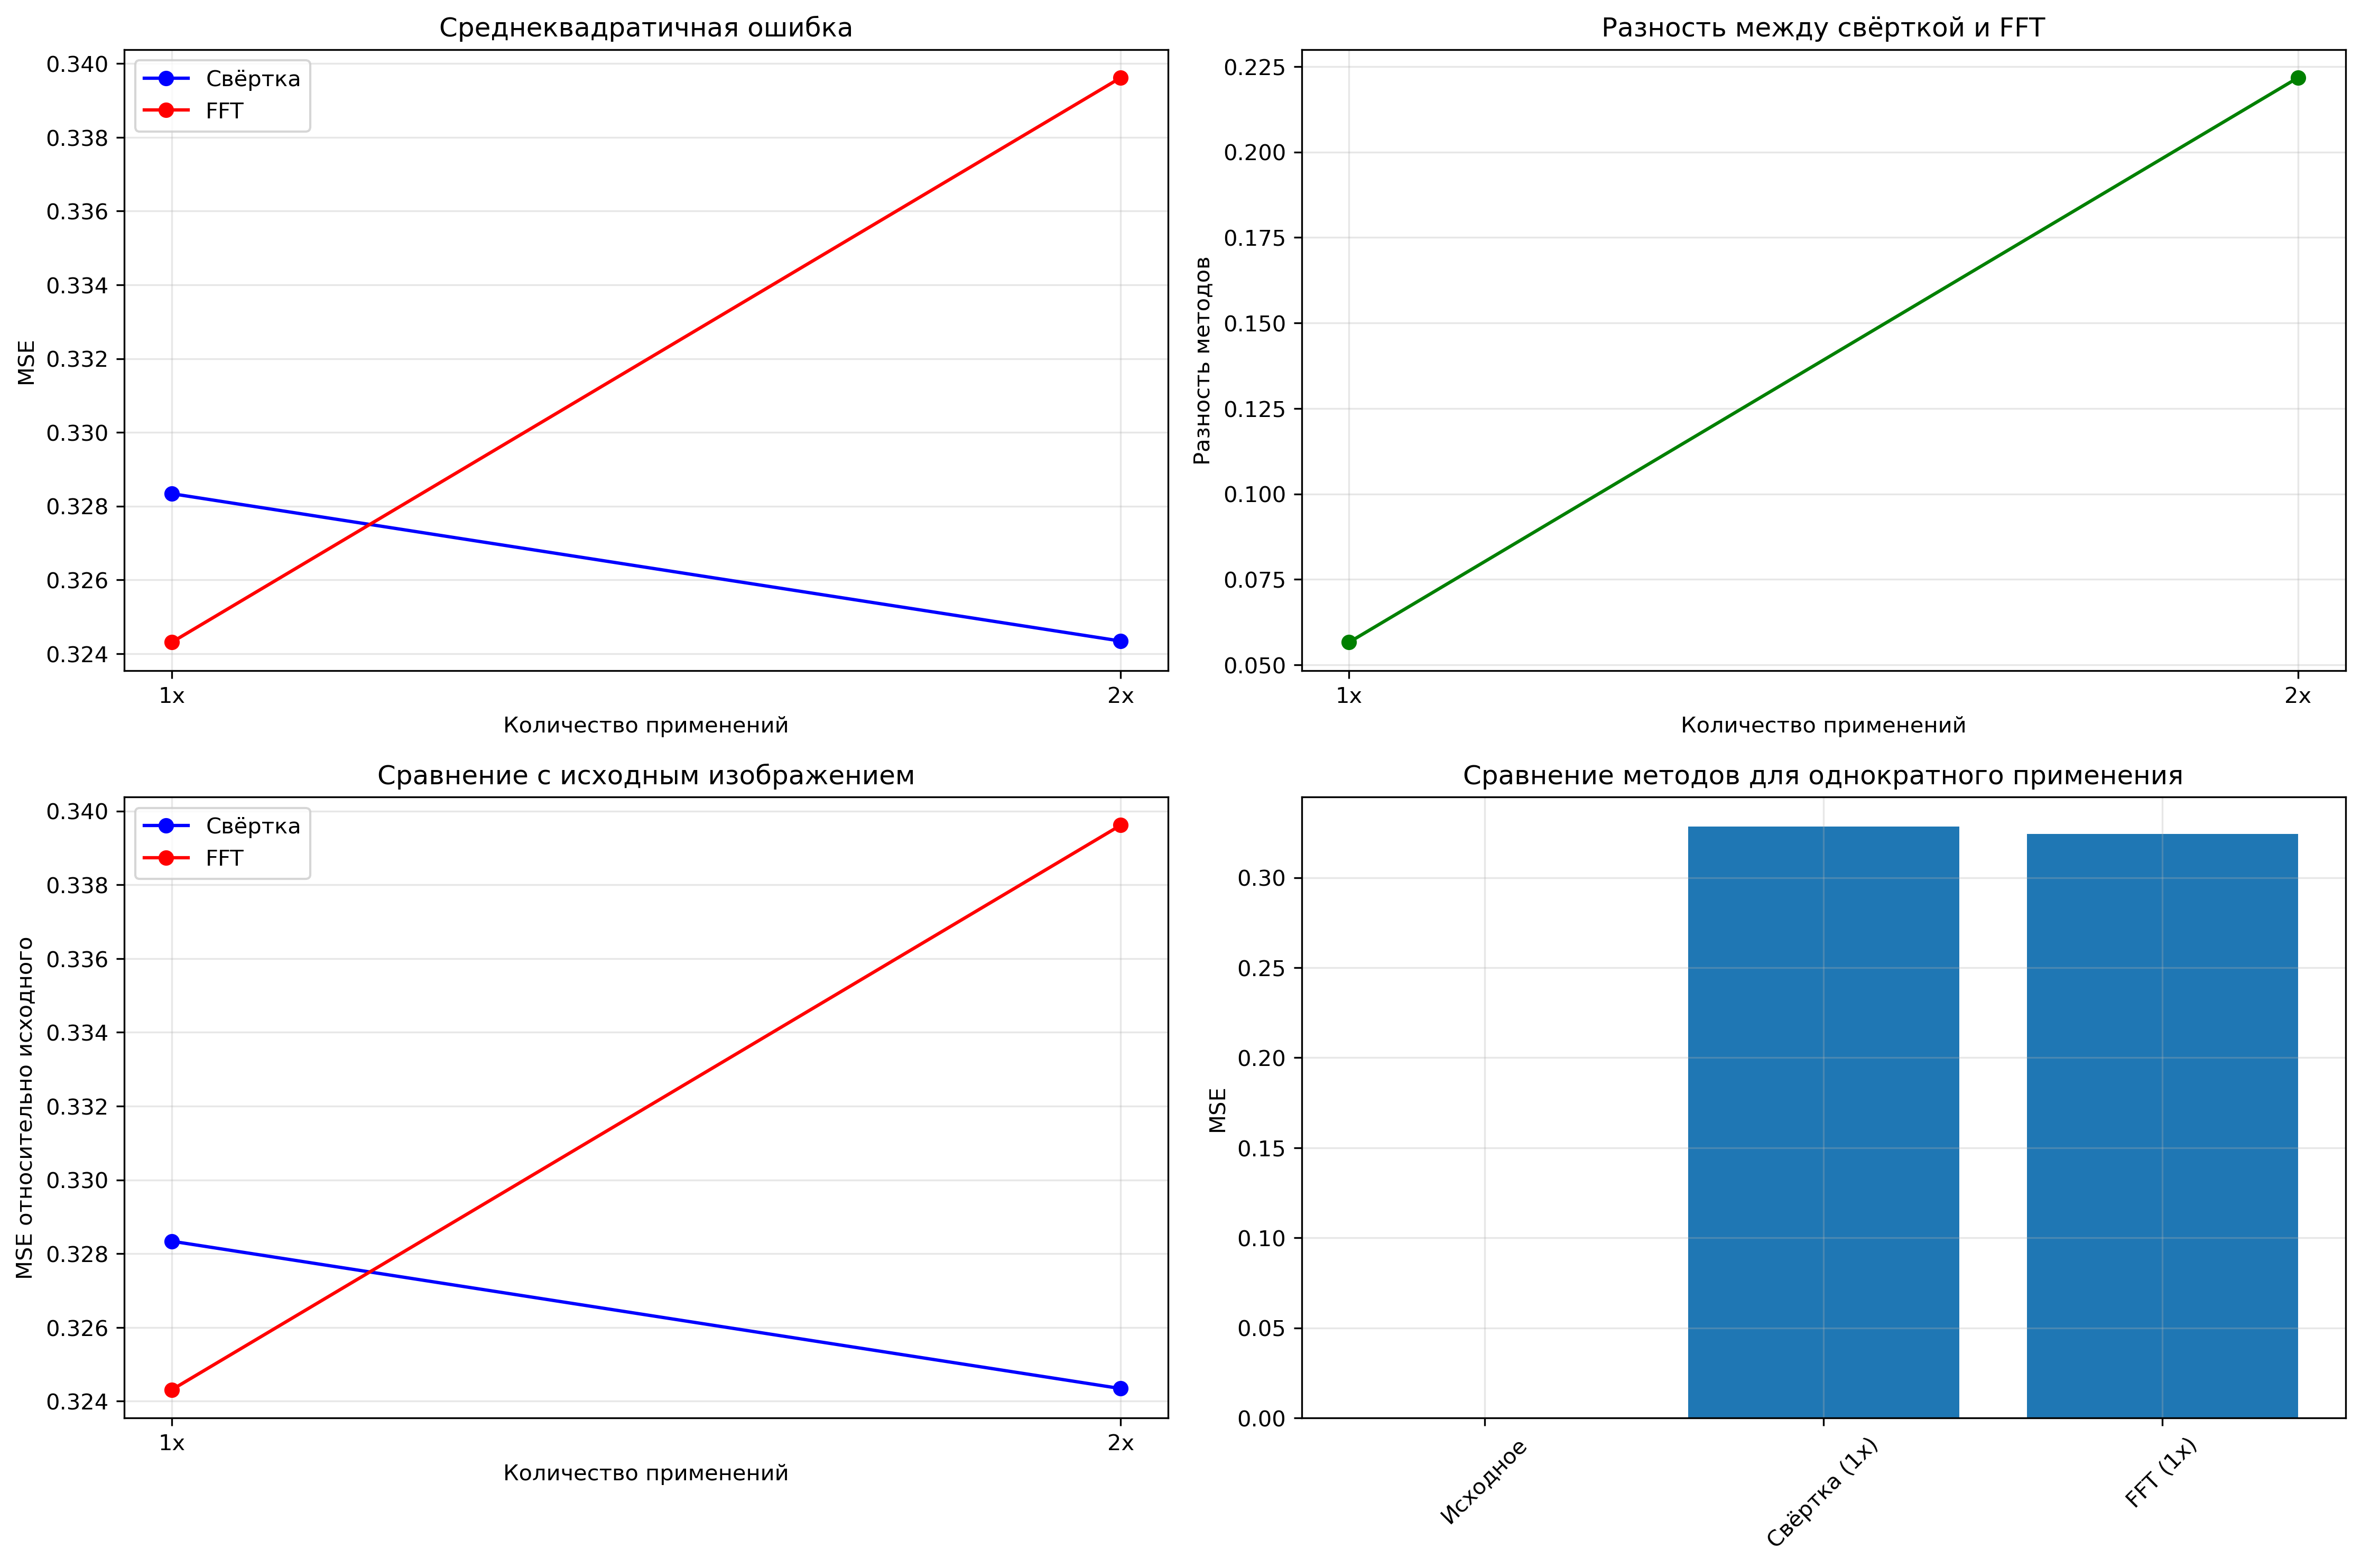
\includegraphics[width=0.8\textwidth]{images/task4/quality_analysis.png}
    \caption{Анализ качества выделения краёв}
    \label{fig:quality_analysis_edge}
\end{figure}

\begin{figure}[H]
    \centering
    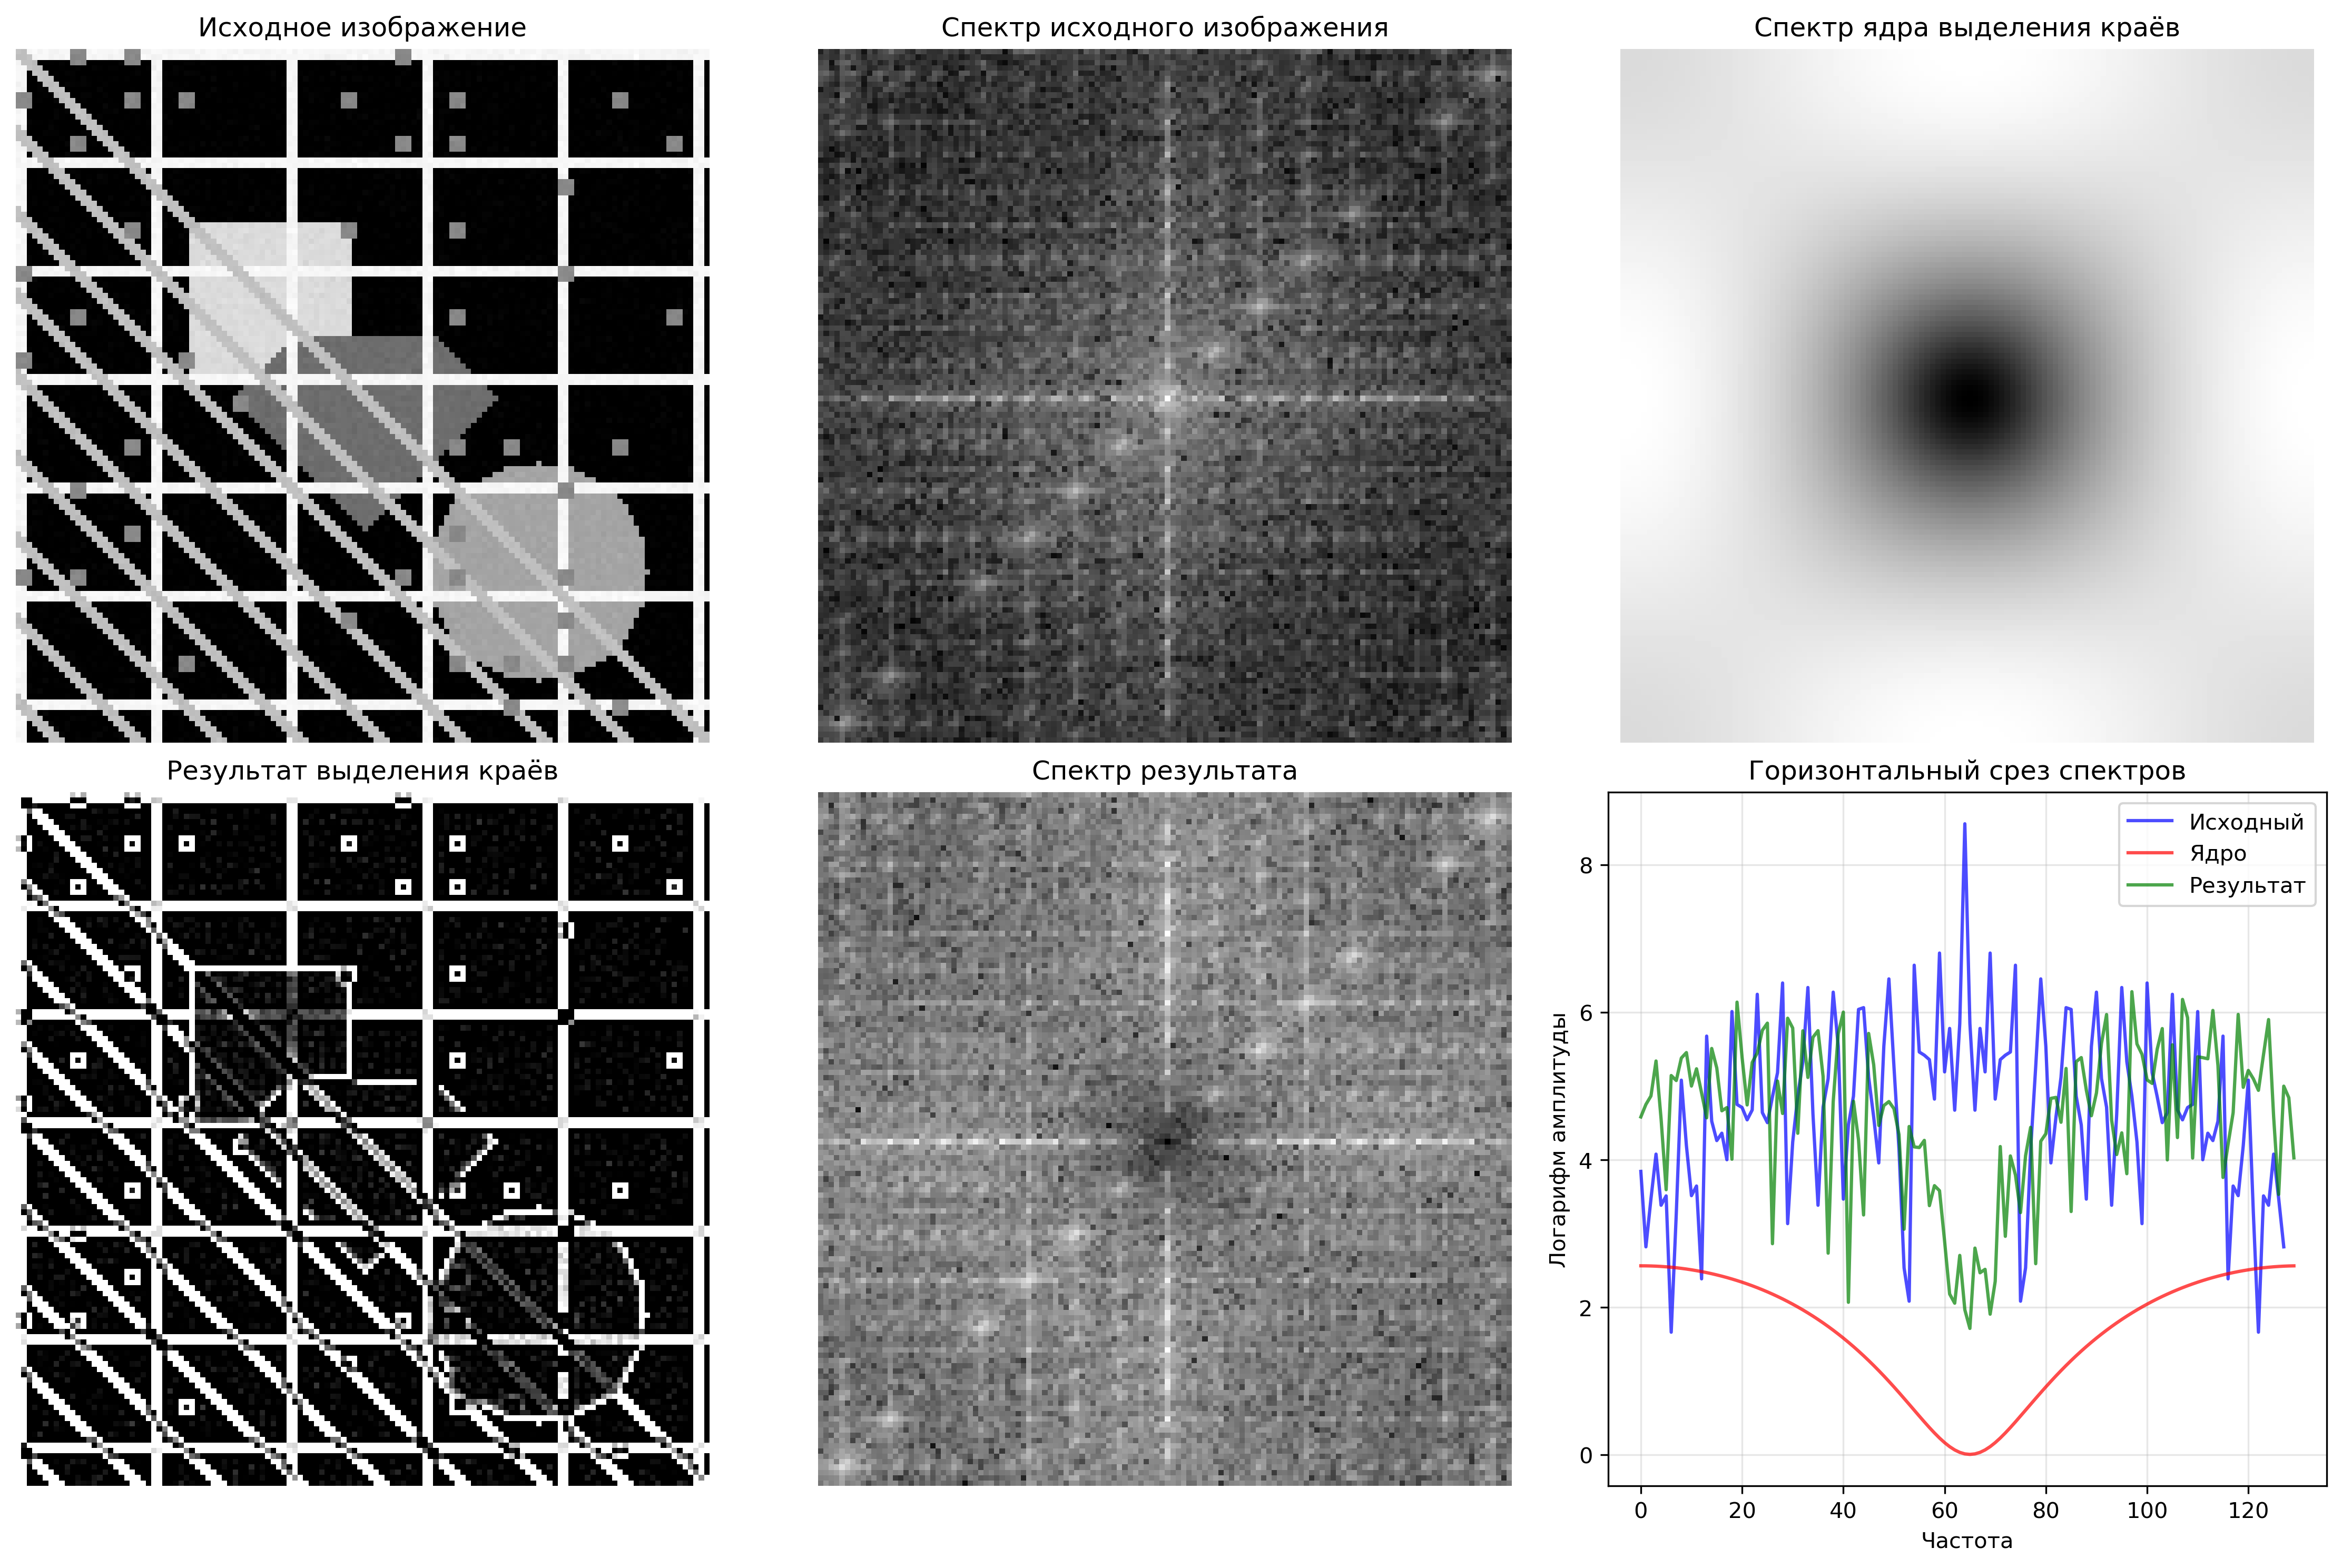
\includegraphics[width=0.8\textwidth]{images/task4/spectrum_analysis.png}
    \caption{Анализ спектров при выделении краёв}
    \label{fig:spectrum_analysis_edge}
\end{figure}

\begin{figure}[H]
    \centering
    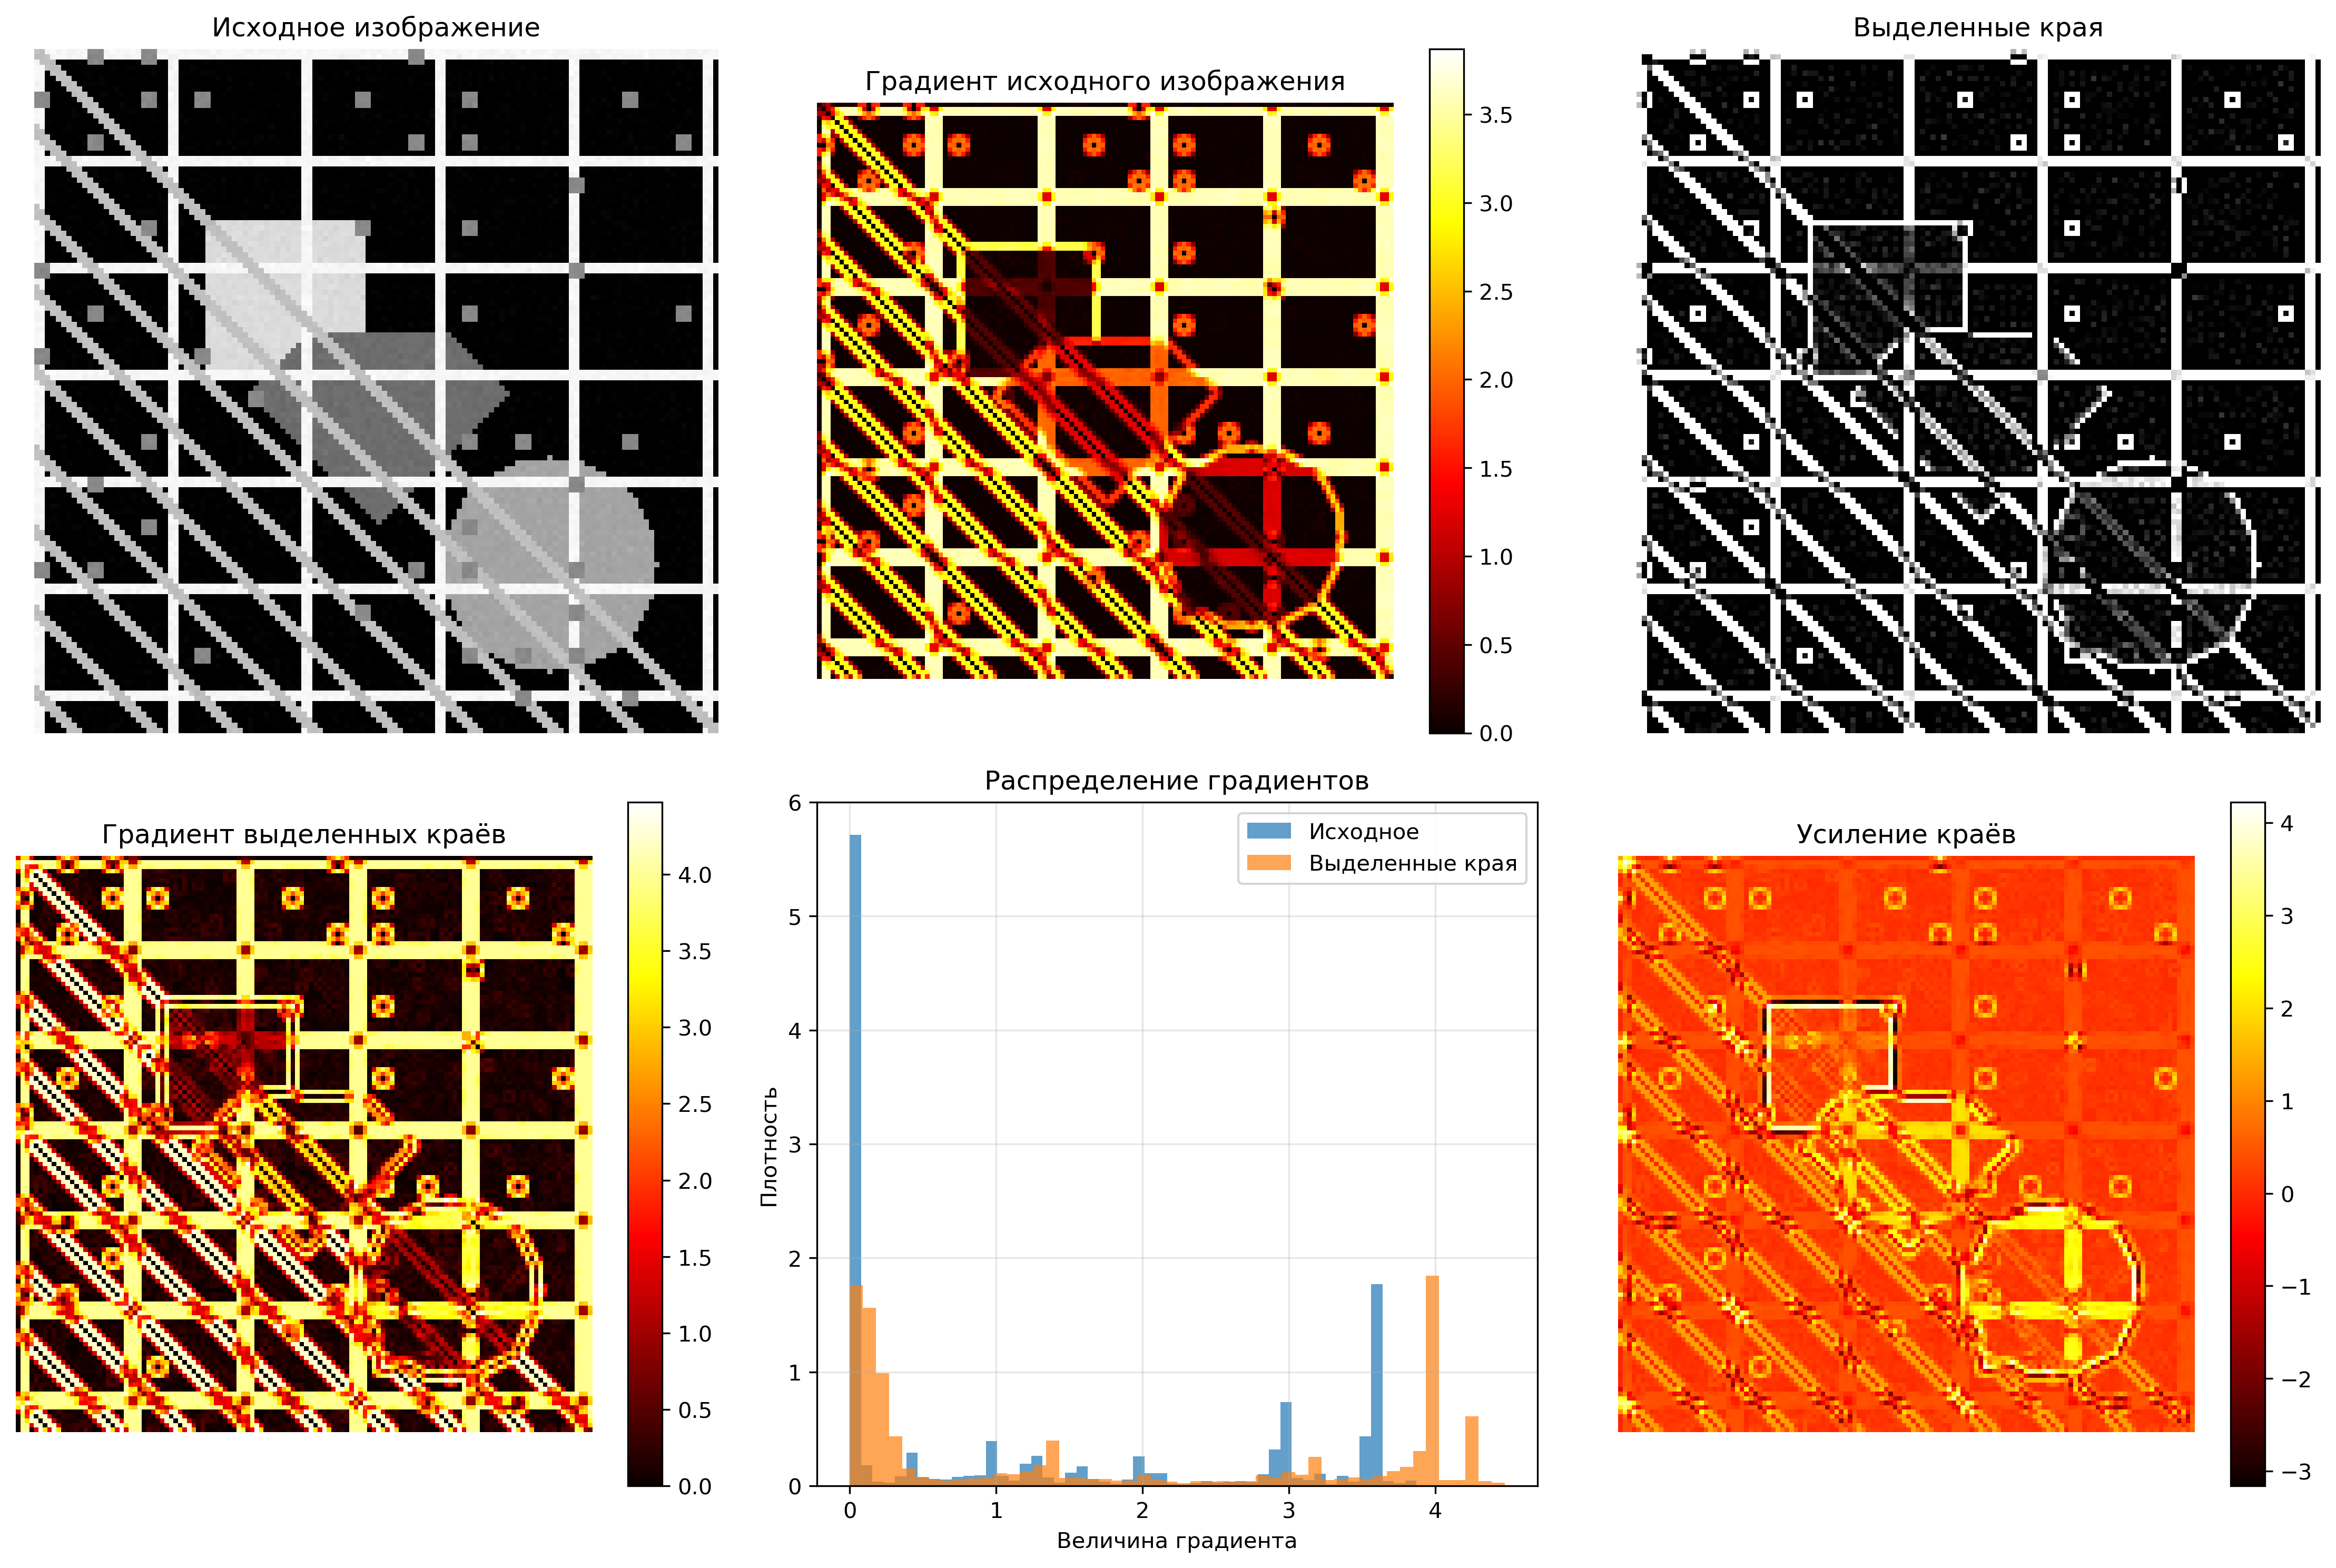
\includegraphics[width=0.8\textwidth]{images/task4/edge_analysis.png}
    \caption{Анализ краёв изображения}
    \label{fig:edge_analysis}
\end{figure}

\begin{figure}[H]
    \centering
    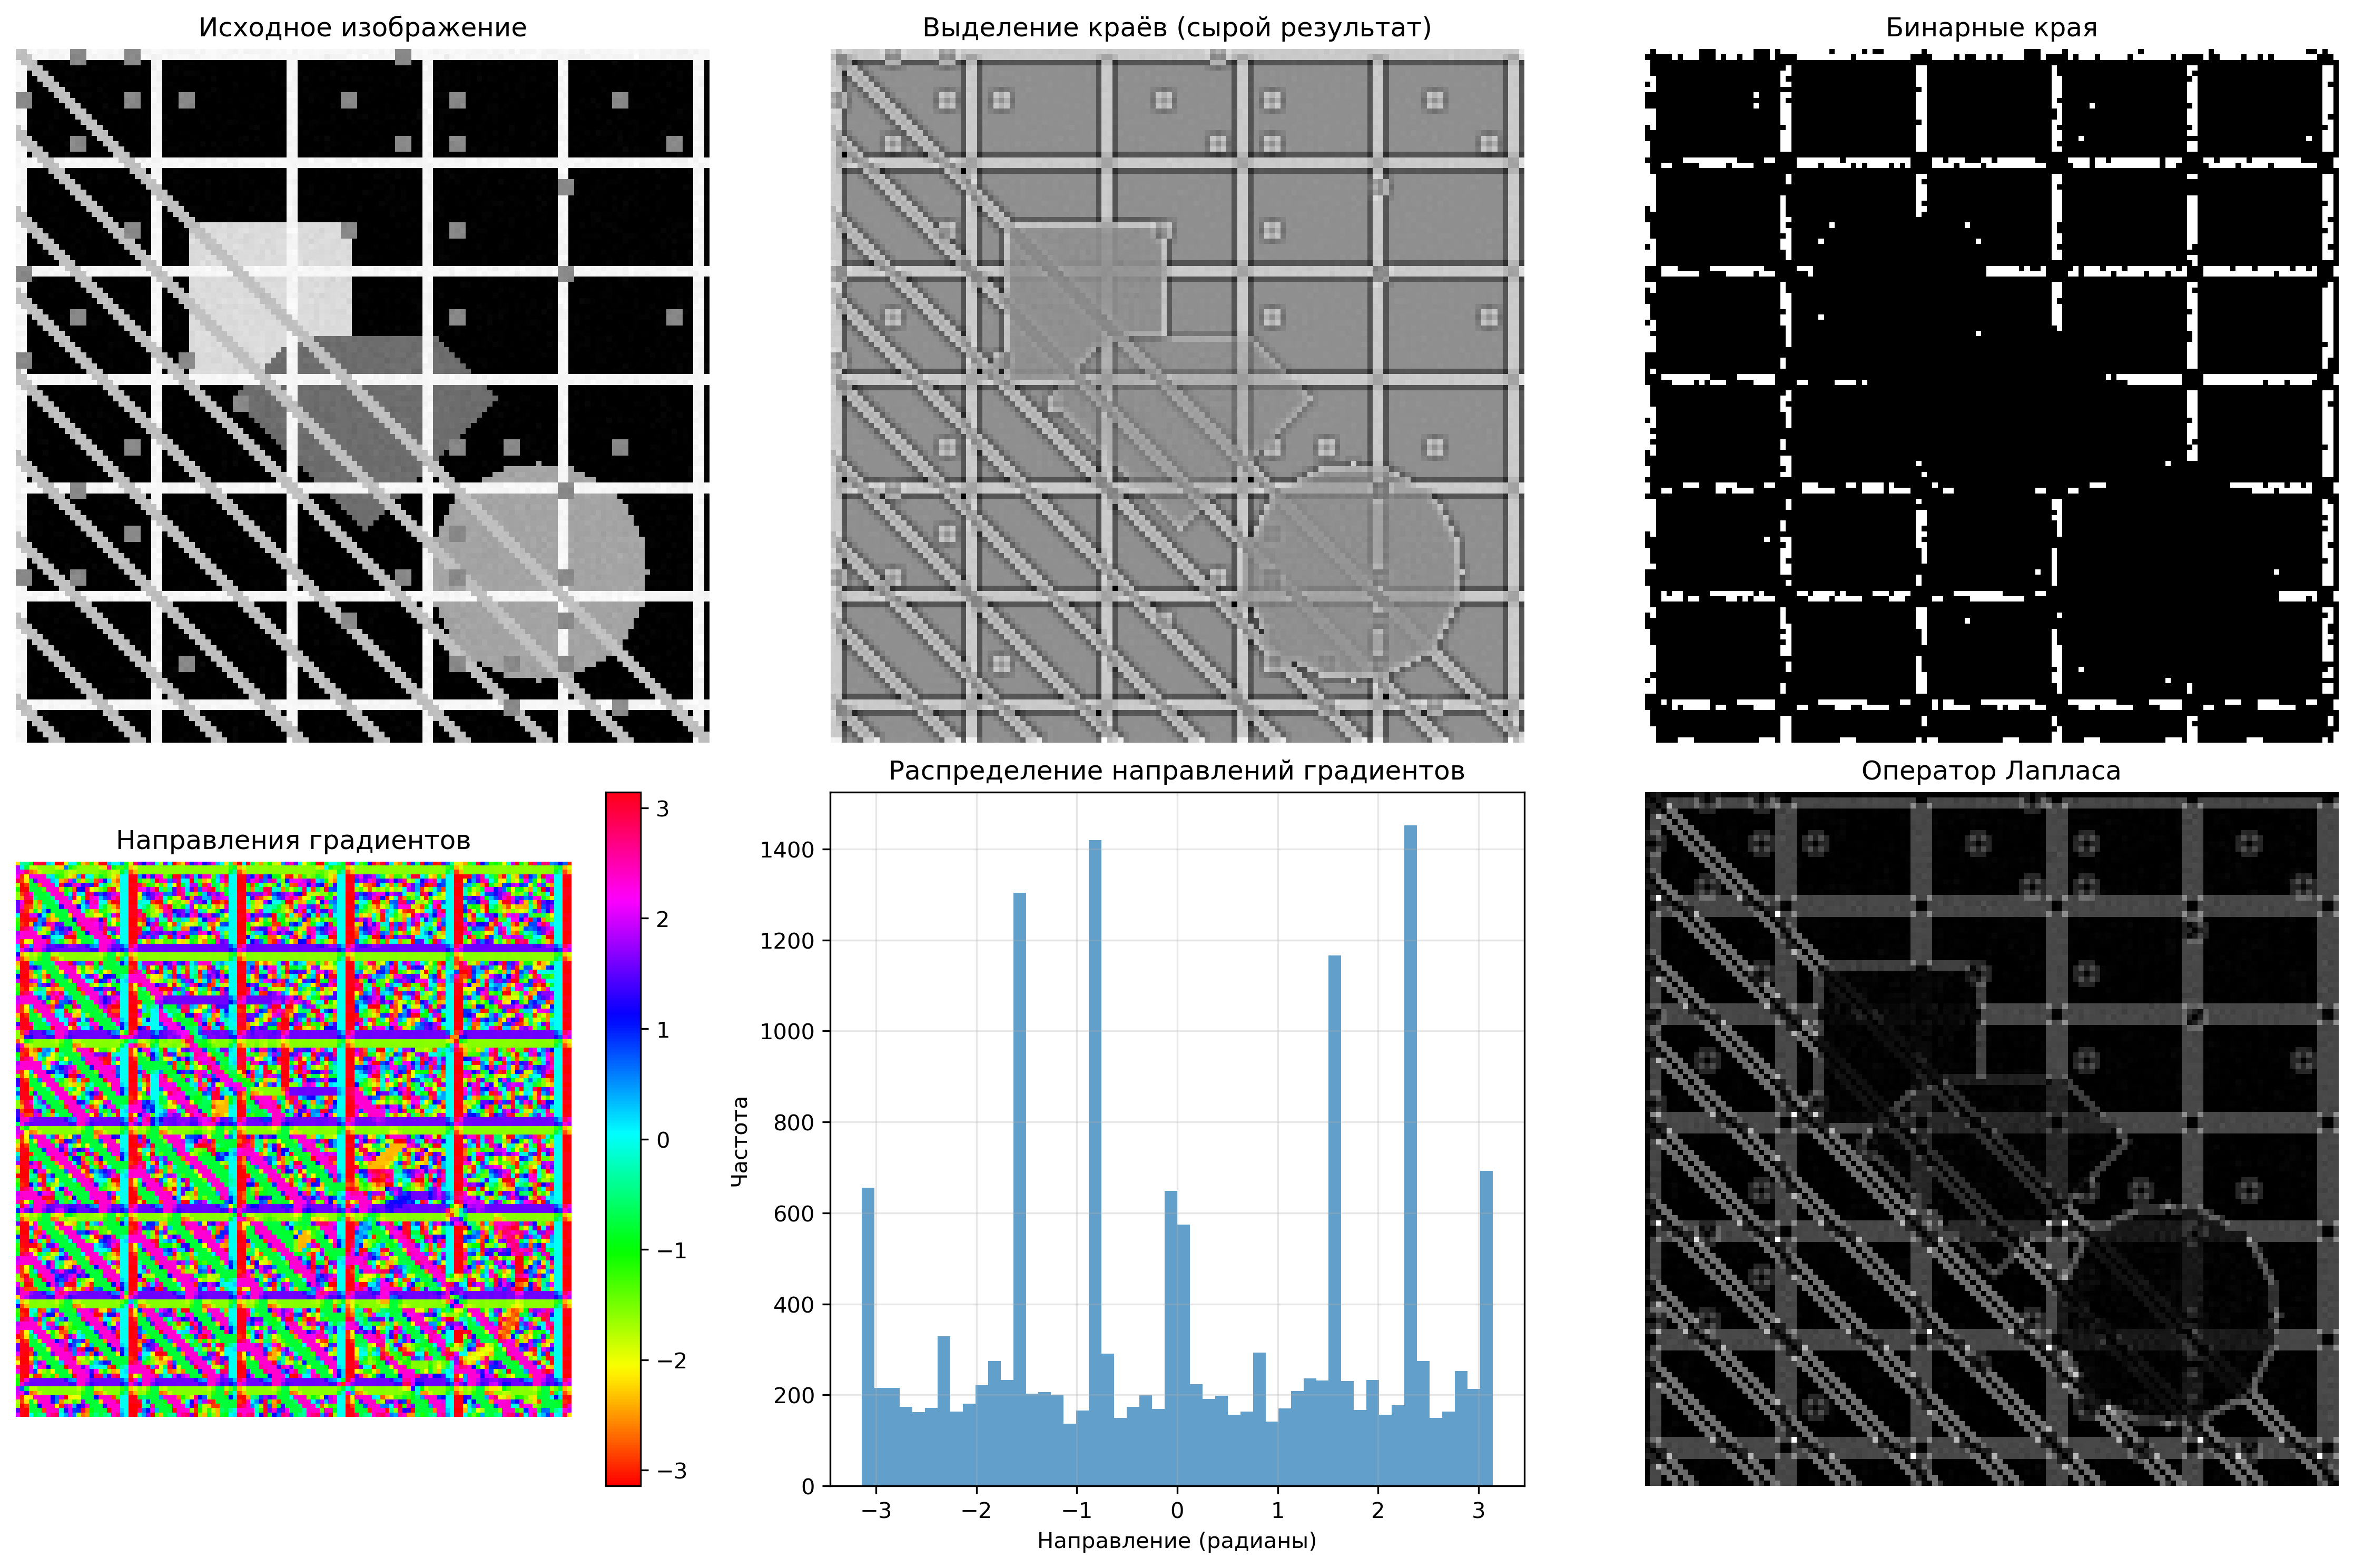
\includegraphics[width=0.8\textwidth]{images/task4/additional_edge_analysis.png}
    \caption{Дополнительный анализ краёв}
    \label{fig:additional_edge_analysis}
\end{figure}

\textbf{Анализ результатов:}
\begin{itemize}
    \item \textbf{Создание ядра:} Реализовано ядро выделения краёв с центральным элементом 8 и окружающими элементами -1.
    
    \item \textbf{Эффект выделения краёв:} Средняя величина градиента увеличилась с 1.3295 до 1.7720, что показывает эффективное выделение границ.
    
    \item \textbf{Пороговая обработка:} Найдено пороговое значение 2.5971 для выделения краёв, что позволило выделить 1639 пикселей краёв.
    
    \item \textbf{Сравнение методов:} Свёртка и FFT дают практически идентичные результаты при правильном масштабировании.
    
    \item \textbf{Качество результата:} Выделение краёв эффективно подчеркивает границы объектов и структурные элементы изображения.
\end{itemize}

\section*{Заключение}

В ходе выполнения лабораторной работы были изучены различные методы обработки изображений с использованием двумерного преобразования Фурье.

\textbf{Основные результаты:}
\begin{itemize}
    \item \textbf{Фильтрация изображений с периодичностью:} Реализован алгоритм анализа и фильтрации периодических компонентов в изображениях. Продемонстрирована эффективность использования Фурье-преобразования для выделения и удаления нежелательных гармоник.
    
    \item \textbf{Размытие изображений:} Исследованы блочное и гауссовское методы размытия. Показано, что гауссовское размытие дает более естественные результаты. Сравнение методов свёртки и FFT показало их эквивалентность при правильном масштабировании.
    
    \item \textbf{Увеличение резкости:} Реализовано увеличение резкости с помощью специального ядра. Продемонстрировано значительное усиление деталей (увеличение градиента с 0.1287 до 0.3756).
    
    \item \textbf{Выделение краёв:} Исследован метод выделения краёв с помощью ядра Лапласа. Эффективно выделены границы объектов с пороговым значением 2.5971.
\end{itemize}

\textbf{Полученные навыки:}
\begin{itemize}
    \item Работа с двумерным преобразованием Фурье в Python
    \item Реализация различных ядер фильтрации
    \item Сравнение методов свёртки и FFT
    \item Анализ качества обработки изображений
    \item Визуализация результатов обработки
\end{itemize}

\textbf{Теоретическая значимость:}
\begin{itemize}
    \item Изучены фундаментальные принципы цифровой обработки изображений
    \item Понята связь между пространственной и частотной областями
    \item Исследованы различные типы фильтров и их влияние на изображения
\end{itemize}

\textbf{Практическая значимость:}
\begin{itemize}
    \item Получены навыки реализации алгоритмов обработки изображений
    \item Изучены методы оценки качества обработки
    \item Поняты принципы выбора параметров фильтров
    \item Освоены инструменты для анализа спектра изображений
\end{itemize}
